%%%%%%%%%%%%%%%%%%%%%%%%%%%%%%%%%%%%%%%%%%%%%%%%%%%%%%%%%%%%%%%%%%%%%%%%%%%%%%%%
% \documentclass[12pt,papel,twoside]{ibtesis}
% \documentclass[12pt,papel,singlespace,oneside]{ibtesis}
% \documentclass[12pt,papel,preprint,singlespace,oneside]{ibtesis}

\documentclass[screen,pagebackref]{ibtesis}
% Antes acá estaba
% \documentclass[12pt,screen,twoside,pagebackref]{ibtesis}


%%%%%%%%%%%%%%%%%%%%% Paquetes extra %%%%%%%%%%%%%%%%%%%%%%%%%%%%%%%%%%%%%%%%%%%
% Por conveniencia: aqu\'{\i} puede cargar todos los paquetes y definir los comandos 
% que necesite
\usepackage{ibextra}
\usepackage{xurl}
\usepackage{caption}
\usepackage{subcaption}
\usepackage{amssymb} 
\usepackage{cancel}
\usepackage[dvipsnames]{xcolor}
\usepackage{listings}
\usepackage{graphicx}
\usepackage{wrapfig}
\usepackage{lscape}
\usepackage{rotating}
\usepackage{epstopdf}
\newcommand{\grad}{^{\circ}}
%\usepackage{hyphen-spanis}
%%%%%%%%%%%%%%%%%%%%%%%%%%%%%%%%%%%%%%%%%%%%%%%%%%%%%%%%%%%%%%%%%%%%%%%%%%%%%%%%
%%%%%%%%%%%%%%%%%%%%% Informacion sobre la tesis %%%%%%%%%%%%%%%%%%%%%%%%%%%%%%%
\title{Conformación digital de haz para recepción de señales satelitales}
\author{Lucas Mariano Grigolato}
\director{Dr. Santiago Hernandez}
\codirector{Ing. Nicolás Catalano}
\carrera{Proyecto Integrador de la Carrera de Ingeniería en Telecomunicaciones}
\grado{Estudiante}
\laboratorio{Departamento de Ingeniería en Telecomunicaciones\\Comisión Nacional de Energía Atómica\\Centro Atómico Bariloche}
\jurado{Ing. Roberto Costantini (INVAP - Instituto Balseiro)\\ 
Dr. Damián Dellavale Clara (CONICET - Instituto Balseiro)}
\palabrasclave{Instituto Balseiro,Conformación de haz, arreglo de antenas en fase, ESPRIT, MUSIC, Muestreo Aleatorio, Aprendizaje Automático, Máquina de Vectores de Soporte, GNU Radio, FPGA}
\keywords{Instituto Balseiro, Beamforming, Phased array antenna, ESPRIT, MUSIC, Random Sampling, Machine Learning, Support vector machine, GNU Radio, FPGA}
% Si queremos poner la fecha manualmente:
\date{17 de Diciembre de 2020}

%%%%%%%%%%%%%%%%%%%%%%%%%%%%%%%%%%%%%%%%%%%%%%%%%%%%%%%%%%%%%%%%%%%%%%%%%%%%%%%%
%\titlepagefalse % Si no quiere compilar la portada descomente esta linea
%\includeonly{apendices} % Compilar s\'{o}lo estos archivos 
\graphicspath{{figs/}} % Lugar donde encontrar las figuras generales (se puede poner uno en cada cap{\'{\i}}tulo)
%%%%%%%%%%%%%%%%%%%%%%%%%%%%%%%%%%%%%%%%%%%%%%%%%%%%%%%%%%%%%%%%%%%%%%%%%%%%%%%%


\begin{document}

% Dentro del environment 'preliminary' va:
% la dedicatoria, resumen, abstract, indices

\begin{preliminary}

    % Escriba su dedicatoria
    \dedicatoria{
        A mi mamá\\
        y a mis hermanos Fer y Palito,\\
        máximos responsables de que haya podido llegar hasta acá.
    }

    %%% \'{I}ndices %%%%

    \begin{abreviaturas}
        \begin{itemize}
            \item ACU: Arreglo Circular Uniforme.
            \item ALU: Arreglo Lineal Uniforme.
            \item ARU: Arreglo Rectangular Uniforme.
            \item BER: Bit Error Rate.
            \item DBF: Digital Beamforming/Beamformer - Conformación/Conformador Digital de Haz.
            \item DOA: Direction of Arrival - Dirección de arribo.
            \item DSP: Digital Signal Processor.
            \item FPGA: Field-Programmable Gate Array - Arreglo de compuertas programable.
            \item LEO: Low Earth Orbit - Baja órbita.
            \item MUSIC: Multiple Signal Classification.
            \item PL: Programmable Logic.
            \item PS: Processing System.
            \item QPSK: Quadrature Phase-Shift Keying.
            \item RF: RadioFrecuencia.
            \item RMSE: Root Mean Square Error.
            \item SDR: Software Defined Radio.
            \item SNR: Signal-to-Noise Ratio - Relación Señal a Ruido.
            \item SVD: Singular Value Decomposition.
            \item SVM: Support Vector Machines.
            \item TLS: Total Least Squares.
            \item UDP: User Datagram Protocol.
        \end{itemize}

    \end{abreviaturas}

    \tableofcontents                %\'{I}ndice

    \listoffigures                  %Figuras

    \listoftables                   %Tablas

    \begin{resumen}%
    Este es el resumen en castellano.\\
    La tesis debe reflejar el trabajo desarrollado, mostrando la metodolog\'{\i}a utilizada, los resultados obtenidos y las conclusiones que pueden inferirse de dichos resultados.
\end{resumen}

\begin{abstract}%
    This is the title in English:\\
    The thesis must reflect the work of the student, including the chosen methodology, the results and the conclusions that those results allow us to draw.
\end{abstract}

\end{preliminary}


\chapter{Introducción}

Las comunicaciones inalámbricas son unas de las tecnologías de mayor crecimiento a lo largo del último siglo.

\subsection{Objetivos de proyecto}\label{subc:objetivos}
\chapter{Conformación de haz}\label{ch:beamforming}
%\chapterquote{Hablaban siempre de dinero y planeaban asaltar un banco}{Domingo Cavallo, 2001}

\section{Conceptos generales}\label{sec:beamforming_congen}

\section{Algoritmos de estimación de dirección de arribo.}\label{sec:beamforming_algoritmos}

\subsection{El algoritmo MUSIC}\label{sec:beamforming_MUSIC}

\subsection{El algoritmo ESPRIT}\label{sec:beamforming_ESPRIT}

\section{Errores en la estimación de dirección de arribo}\label{sec:beamforming_errores}



\chapter{Algoritmos de estimación de dirección de arribo.}\label{ch:doaest}
\chapterquote{Son nuestras elecciones, Harry, las que muestran lo que somos, mucho más que nuestras habilidades.}{Albus Dumbledore}

\section{Introducción}\label{subc:doaest_intro}
Al momento de diseñar un conformador de haz adaptativo uno de los pasos más importantes es definir el algoritmo de estimación de dirección de arribo (DOA). Estos algoritmos explotan las propiedades estadísticas de las señales recibidas por los elementos del arreglo de antenas y entregan la dirección de arribo en las dimensiones correspondientes según el tipo de arreglo con el que se trabaje. El estudio de los algoritmos de estimación de DOA data de la Segunda Guerra Mundial con la aparición del conformador de Bartlett \cite{bib:2decadesbeamforming}, el cual consiste en hacer un escaneo de potencia en el dominio de búsqueda identificando la dirección que maximiza la potencia de salida. Este algoritmo pertenece al grupo de algoritmos basados en el análisis espectral, los cuales tienen la desventaja de que su resolución depende fuertemente del ancho del haz sintetizado y que requieren de una búsqueda en una o dos dimensiones para realizar la estimación, lo cual reduce su viabilidad si es que se los quiere utilizar para seguimientos de objetivos en tiempo real. Posteriormente, nuevos métodos fueron propuestos, mejorando así el desempeño en la detección y en la eficiencia, como son los métodos basados en la separación de subespacios de señal y ruido, los cuales se basan en explotar las propiedades geométricas del arreglo de antenas y tienen la ventaja de que su resolución no está limitada a la apertura del mismo. Dentro de este tipo de algoritmos de estimación de DOA, los algoritmos \emph{Multiple Signal Classification} (\emph{MUSIC}) y \emph{Estimation of Signal Parameters via Rotational Invariance Techniques} (\emph{ESPRIT}) son dos de los más importantes, y son, además, los que se estudiarán a lo largo de este capítulo.

La disponibilidad en la utilización de un algoritmo dependerá fuertemente del tipo de arreglo con el que se cuente para la implementación, es por esto que a la hora de elegir la manera de disponer los elementos del arreglo para realizar un conformador de haz adaptativo hay que tener en cuenta cuáles distribuciones son aquellas que brindan mejores opciones para la estimación de DOA. Para dar un ejemplo, el algoritmo \emph{Root-MUSIC} tiene un costo computacional relativamente bajo para lograr la estimación, ya que su solución consiste simplemente en encontrar las raíces de un polinomio, pero solo funciona en arreglos lineales uniformes, por ende solo permite estimar la dirección de arribo en una única dimensión.

Vale la pena aclarar que las técnicas utilizadas en este capítulo permiten, también, obtener información de otros parámetros de las señales arribantes, como pueden ser la frecuencia de portadora de las mismas o la cantidad de fuentes de señal que está recibiendo el arreglo de antenas, razón por la cual estos algoritmos resultan muy versátiles en el mundo del procesamiento estadístico de señales.

Para realizar el análisis de los algoritmos mencionados se deberá primero definir un modelo de datos común que refleje matemáticamente cómo pueden ser representadas las muestras obtenidas por el arreglo de antenas.

\subsection{Modelo de datos}\label{subc:doaest_datamodel}

Antes de especificar el modelo de datos es necesario aclarar que para los próximos análisis se considerará que el medio de transmisión es lineal, y, por ende, vale el principio de superposición. Debido a esto, si consideramos que a un arreglo de M elementos está llegando un número $D$ de señales desde distintas direcciones, la Ecuación \ref{eq:beamforming_singlesignal} puede reescribirse como:
\begin{equation}
    \bar{x} (t)  =\sum_{d=0}^{D-1} \bar{a}(\theta_d,\varphi_d)\cdot s_d(t) + \bar{w}(t),
\end{equation}
donde $\bar{a}(\theta_d,\varphi_d)$ con $d=0,1,...,D-1$ es el vector de apuntamiento que corresponde a la señal $s_d(t)$ llegando al arreglo con dirección $(\theta_d,\varphi_d)$, la cual es medida en el elemento de referencia. Esta ecuación puede reescribirse en forma matricial haciendo:
\begin{equation}
    \bar{x} (t) = \mathbf{A}(\theta,\varphi) \bar{s}(t) + \bar{w}(t),
\end{equation}
\begin{equation}
    \mathbf{A(\theta,\varphi)} = \begin{bmatrix}
        \bar{a}(\theta_0,\varphi_0) & \bar{a}(\theta_1,\varphi_1) & \cdots & \bar{a}(\theta_{D-1},\varphi_{D-1})
    \end{bmatrix}_{(M\times D)}
\end{equation}
donde $\bar{s}(t)=[s_0(t), s_1(t), \cdots, s_{D-1}(t)]^T$.

Si tomamos una instantánea de las muestras del arreglo vemos que las mismas pueden representarse como un vector de números complejos de la siguiente manera:
\begin{gather*}
    \bar{x}=\mathbf{A}(\theta,\varphi)\bar{s}+\bar{w},\\
    \begin{bmatrix}
        x_0    \\
        x_1    \\
        \vdots \\
        x_{M-1}
    \end{bmatrix}_{(M\times 1)} = \begin{bmatrix}
        \vphantom{\begin{bmatrix}
                x_0    \\
                x_1    \\
                \vdots \\
                x_{M-1}
            \end{bmatrix}} \bar{a}(\theta_0,\varphi_0) & \bar{a}(\theta_1,\varphi_1) & \cdots & \bar{a}(\theta_{D-1},\varphi_{D-1})
    \end{bmatrix}_{(M\times D)}
    \begin{bmatrix}
        s_0    \\
        s_1    \\
        \vdots \\
        s_{D-1}
    \end{bmatrix}_{(D\times 1)} +
    \begin{bmatrix}
        w_0    \\
        w_1    \\
        \vdots \\
        w_{M-1}
    \end{bmatrix}_{(M\times 1)}
\end{gather*}

A partir de esto podemos ver que el vector de muestras $\bar{x}$ pertenece a $\mathbb{C}^M$. Además, en ausencia de ruido, cada vector de muestras puede expresarse como combinación lineal de los vectores de $\mathbf{A}$, siendo los elementos de $\bar{s}$ los coeficientes de esta combinación. Por ende, si $\bar{w}=\bar{0}$, las muestras estarán confinadas en un subespacio de dimensión $D$ dentro de $\mathbb{C}^M$, generado por las columnas de $\mathbf{A}$, las cuales conforman una base del \emph{subespacio de señal} $\mathcal{S}_S$ \cite{bib:esprit_roy}. Si definimos como $\mathfrak{A}$ al conjunto que contiene a todos los posibles vectores de apuntamiento, para el caso en el que la dirección de arribo es bidimensional, estos vectores definirán una superficie con forma de ``sábana'' en $\mathbb{C}^M$, y en el caso unidimensional definirán una curva cerrada. Identificar cuáles de todos los vectores de $\mathfrak{A}$ conforman la base del subespacio de señal corresponde a encontrar las intersecciones entre la superficie $M$-dimensional formada por $\mathfrak{A}$ y el subespacio de señal \cite{bib:music_schmidt}. En la Figura \ref{fig:doaest_arraymanifold} se muestra una representación para el caso de estimación de DOA unidimensional, con $D=2$ y $M=3$. Si se supone que la función que mapea las posibles direcciones de arribo $(\theta,\varphi)$ a elementos de $\mathfrak{A}$ es inyectiva, encontrar los vectores de $\mathbf{A}$ equivale a encontrar las direcciones de arribo de las $D$ señales recibidas. Esto puede lograrse mediante un diseño apropiado del arreglo de antenas \cite{bib:esprit_roy}. La dificultad radica ahora en definir $\mathcal{S}_S$ a partir de las muestras obtenidas.
\begin{figure}[ht!]
    \centering
    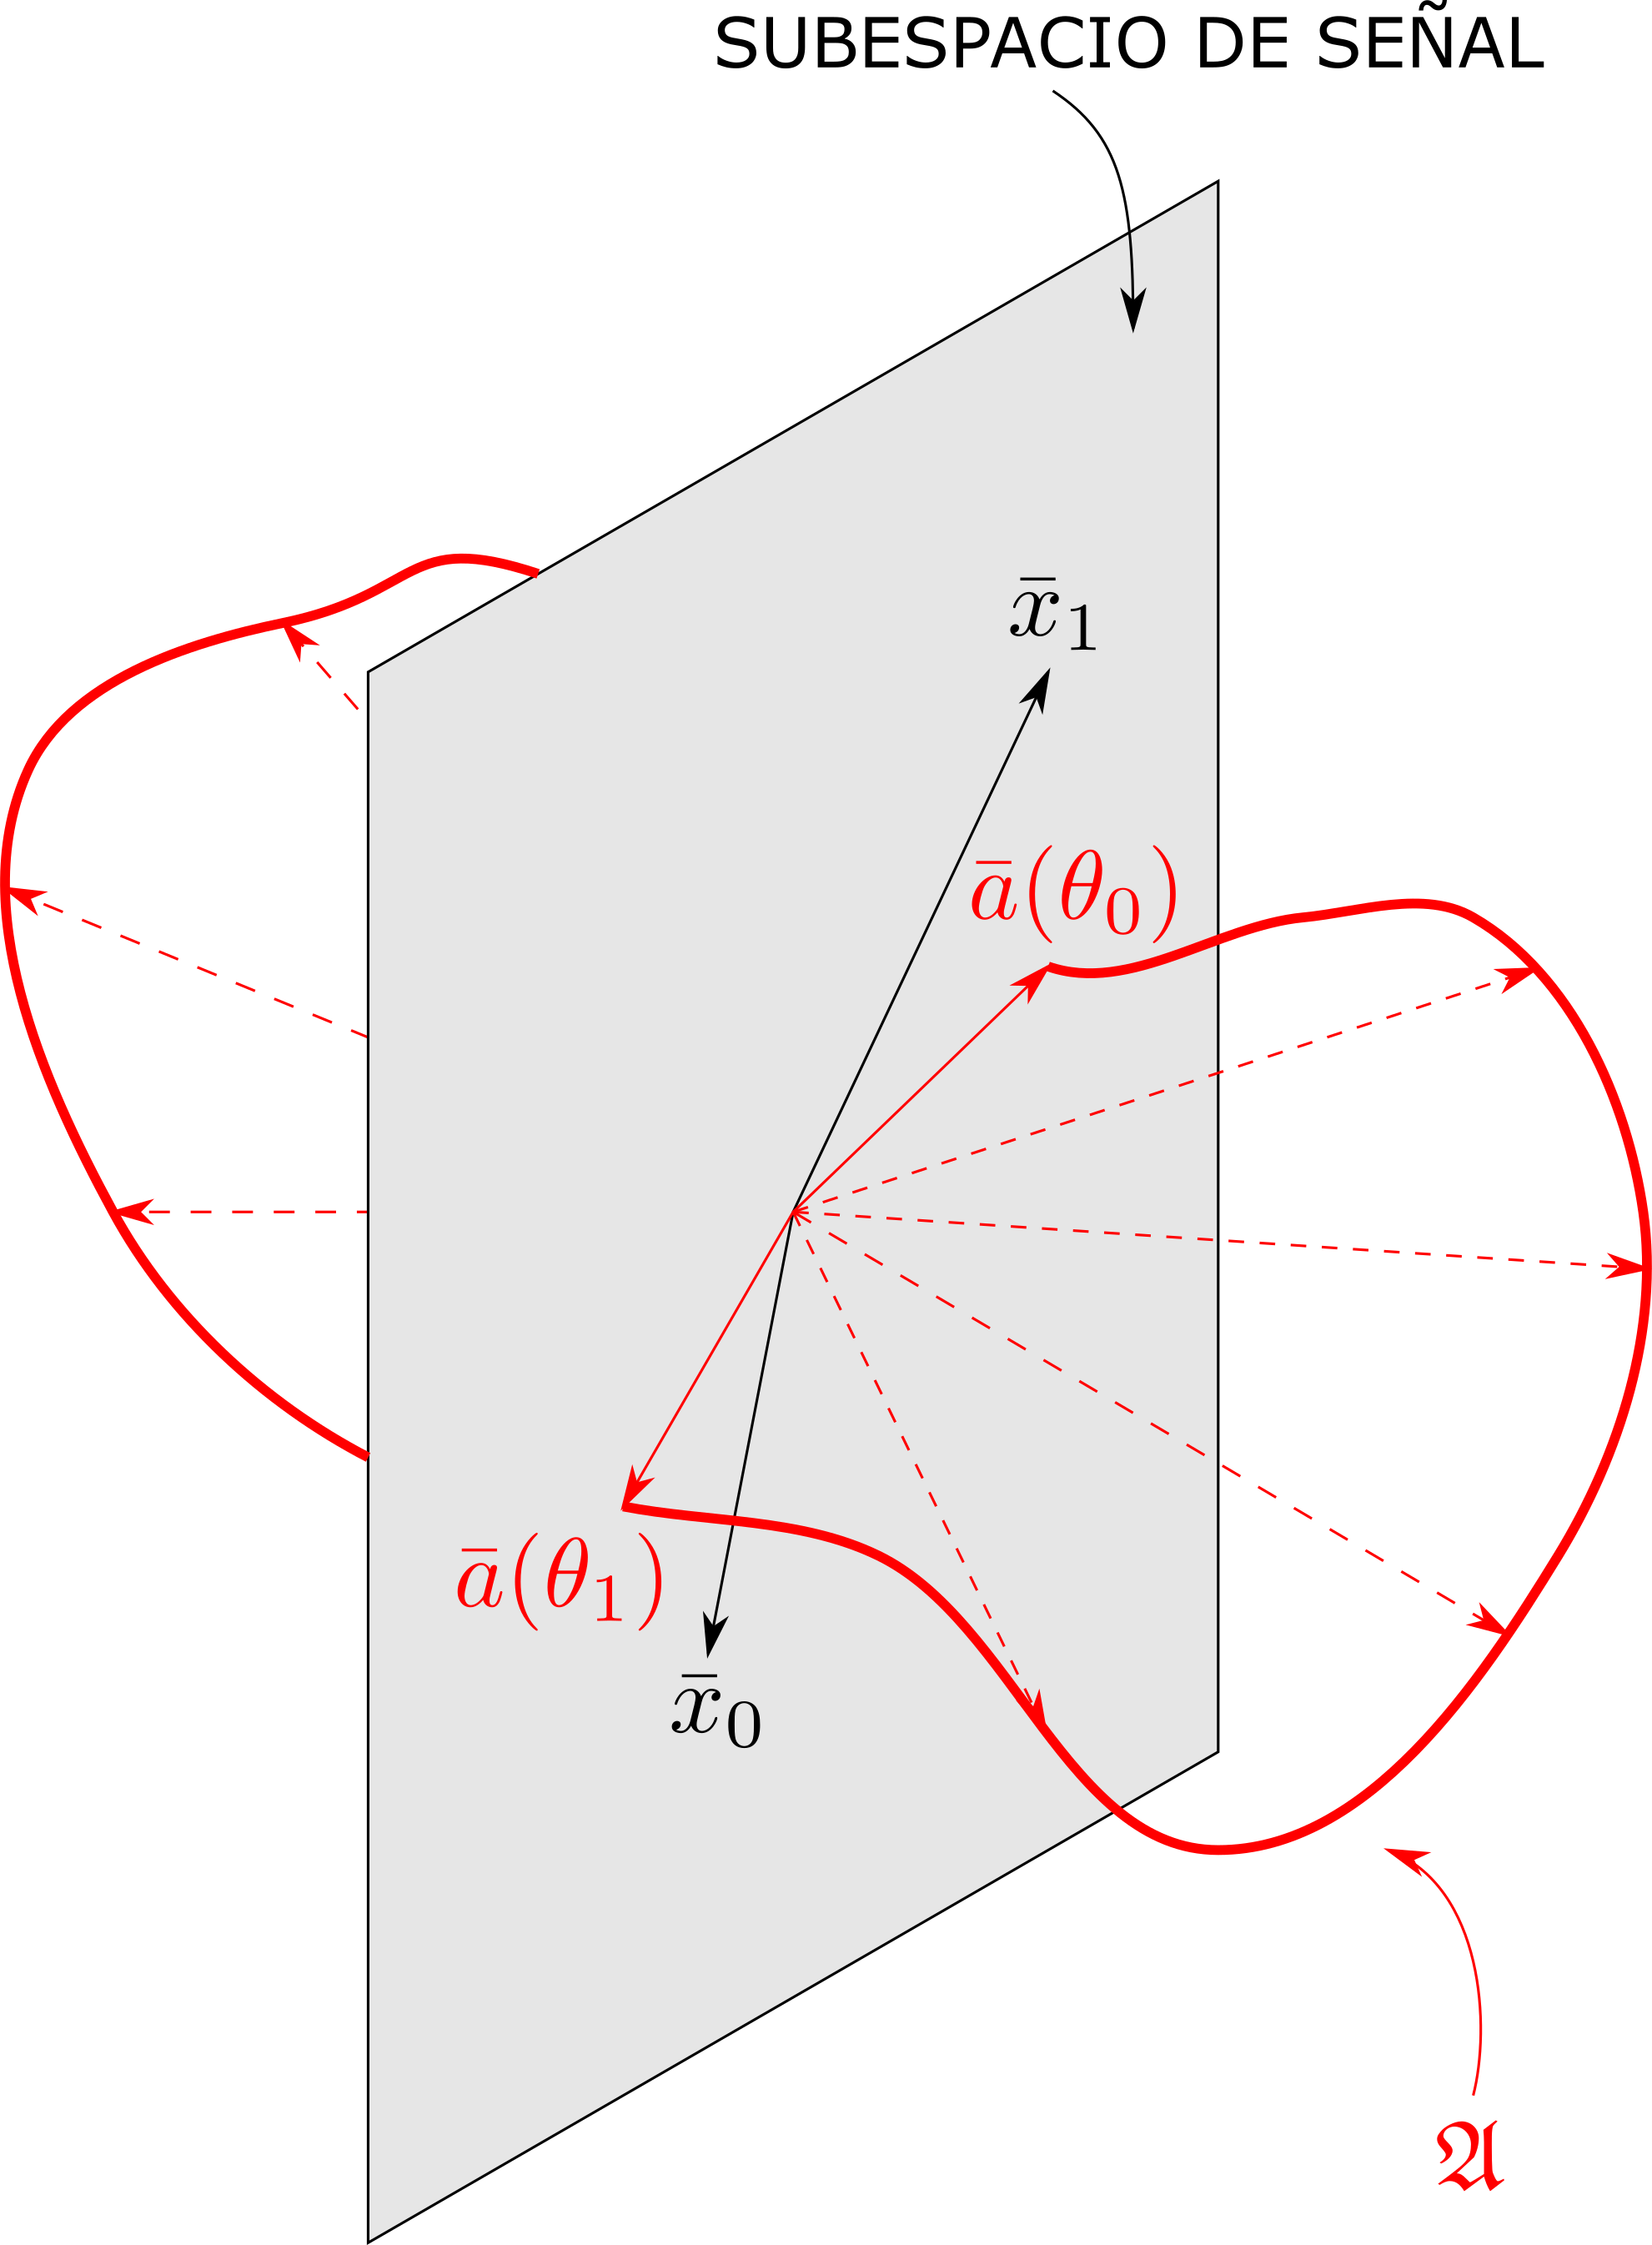
\includegraphics[width=0.7\linewidth]{images/03-DOAEst/arraymanifold.png}
    \caption{Representación geométrica de la estimación de DOA mediante la intersección del conjunto $\mathfrak{A}$ con el subespacio de señal para el caso de DOA unidimensional, con $D=2$ y $M=3$.}
    \label{fig:doaest_arraymanifold}
\end{figure}

\subsubsection{La matriz de covarianza $\mathbf{R_{XX}}$}

Al muestrear digitalmente cada elemento del arreglo tendremos el equivalente a un vector de muestras por cada período de muestreo. Si se quiere representar a todas las muestras tomadas durante $N$ períodos de muestreo se puede escribir:
\begin{gather}
    \mathbf{X}_{(M\times N)} = \mathbf{A(\theta,\varphi)}_{(M\times D)}\times \mathbf{S}_{(D\times N)} + \mathbf{W}_{(M\times N)}    \label{eq:doaest_x}\\
    \mathbf{X}=
    \begin{bmatrix}
        x_0^0     & x_0^1  & \cdots & x_0^{N-1}     \\
        x_1^0     & \ddots &        & \vdots        \\
        \vdots    &        & \ddots & \vdots        \\
        x_{M-1}^0 & \cdots & \cdots & x_{M-1}^{N-1}
    \end{bmatrix},\quad
    \mathbf{S}=\begin{bmatrix}
        s_0^0     & s_0^1  & \cdots & s_0^{N-1}     \\
        s_1^0     & \ddots &        & \vdots        \\
        \vdots    &        & \ddots & \vdots        \\
        s_{D-1}^0 & \cdots & \cdots & s_{D-1}^{N-1}
    \end{bmatrix},\quad
    \mathbf{W}=\begin{bmatrix}
        w_0^0     & w_0^1  & \cdots & w_0^{N-1}     \\
        w_1^0     & \ddots &        & \vdots        \\
        \vdots    &        & \ddots & \vdots        \\
        w_{M-1}^0 & \cdots & \cdots & w_{M-1}^{N-1}
    \end{bmatrix}\nonumber
\end{gather}

Para simplificar la notación a partir de ahora se indicará a la matriz de vectores de apuntamiento simplemente como $\mathbf{A}$.

A partir de esto podemos encontrar la matriz de covarianza de las muestras haciendo:
\begin{align}
    \mathbf{R_{XX}} & =\overline{\mathbf{XX}^H}=\overline{(\mathbf{AS}+\mathbf{W})(\mathbf{AS}+\mathbf{W})^H}=\overline{(\mathbf{AS}+\mathbf{W})(\mathbf{S}^H\mathbf{A}^H+\mathbf{W}^H)}\nonumber      \\
                    & = \mathbf{A}\overline{\mathbf{SS}^H}\mathbf{A}^H + \cancel{\mathbf{A}\overline{\mathbf{SW}^H}}+\cancel{\overline{\mathbf{WS}^H}\mathbf{A}^H} + \overline{\mathbf{WW}^H}\nonumber \\
                    & = \mathbf{AR_{SS}A}^H+\mathbf{R_{WW}}=\mathbf{AR_{SS}A}^H+\sigma^2_w\mathbf{I}_M
    \label{eq:doaest_rxx_teor}
\end{align}
donde se supuso que las señales pueden ser modeladas como procesos estocásticos estacionarios y de media cero, y que el ruido es aditivo, blanco y gaussiano, de manera tal que la correlación entre la señal y el ruido es nula. La matriz $\mathbf{R_{WW}}$ es la matriz de autocorrelación del ruido, siendo $\mathbf{I}_M$ la matriz identidad de tamaño $M\times M$ y $\sigma^2_w=\mathbf{E}\{|w[n]|^2\}$ el nivel de potencia de ruido. Es necesario aclarar que la operación $\overline{\mathbf{XX}^H}$ consiste en realizar el promedio entre las matrices obtenidas al multiplicar cada uno de los vectores columna de $\mathbf{X}$ por su transpuesto conjugado, es decir:
\begin{equation}
    \mathbf{R_{XX}}= \lim_{N\rightarrow\infty} \frac{1}{N} \sum_{n=0}^{N-1}\bar{x}^n(\bar{x}^n)^H,
\end{equation}
siendo $\bar{x}^n$ la columna $n$-ésima de la matriz $\mathbf{X}$. En este análisis se considera la matriz de correlación teórica, la cual requiere de infinitas muestras para poder ser obtenida. En la práctica, la matriz de correlación $\mathbf{R_{XX}}$ debe ser estimada a partir de las muestras obtenidas haciendo \cite{bib:Manolakis_ch9.6}:
\begin{equation}
    \mathbf{\hat{R}_{XX}}=\frac{1}{N} \mathbf{XX}^H
    \label{eq:doaest_rxx_est}
\end{equation}
siendo $N$ la cantidad de muestras tomadas en la ventana temporal de medición. En lo que resta del análisis se seguirá considerando la correlación teórica, debiendo el lector tomar las respectivas consideraciones.

Debido a que los vectores de $\mathbf{A}$ definen la base del subespacio de señal, la matriz $\mathbf{AR_{SS}A}^H$ de tamaño $M\times M$ tiene rango $D$, por lo que es de rango incompleto, a diferencia de $\mathbf{R_{WW}}$ que es de rango completo. Si se considera que las señales que conforman la matriz $\mathbf{S}$ no están correlacionadas entre sí, la matriz de autocorrelación de señal $\mathbf{R_{SS}}$ es de la forma:
\begin{equation}
    \mathbf{R_{SS}}=
    \begin{bmatrix}
        |s_0|^2 & 0       & \cdots & 0           \\
        0       & |s_1|^2 &        & \vdots      \\
        \vdots  &         & \ddots & \vdots      \\
        0       & \cdots  & \cdots & |s_{D-1}|^2
    \end{bmatrix}
    \label{eq:doaest_rss}
\end{equation}
siendo cada elemento de la diagonal la potencia de cada una de las señales.

Si se aplica la descomposición en autovalores a la matriz $\mathbf{R_{XX}}$, esta puede escribirse como \cite{bib:Manolakis_ch9.6}:
\begin{gather}
    \mathbf{R_{XX}}= \mathbf{E\Lambda E}^H,    \label{eq:doaest_eigendesc}\\
    \mathbf{\Lambda}=    \begin{bmatrix}
        \lambda_0 & 0         & \cdots & 0             \\
        0         & \lambda_1 &        & \vdots        \\
        \vdots    &           & \ddots & \vdots        \\
        0         & \cdots    & \cdots & \lambda_{M-1}
    \end{bmatrix},\quad
    \mathbf{E}=\begin{bmatrix}
        \bar{e}_0 & \bar{e}_1 & \cdots & \bar{e}_{M-1}
    \end{bmatrix}\nonumber
\end{gather}
donde $\lambda_0\geq \lambda_1 \geq \cdots \geq \lambda_{M-1}$ son los autovalores de $\mathbf{R_{XX}}$ en orden descendente y $\bar{e}_0$, $\bar{e}_1$, ..., $\bar{e}_{M-1}$ sus correspondientes autovectores. Los $D$ autovalores más grandes serán iguales a la suma de los autovalores de $\mathbf{AR_{SS}A}^H$ más los autovalores de $\mathbf{R_{WW}}$, los cuales son todos iguales. Los $M-D$ autovalores más chicos tendrán el mismo valor que los autovalores de $\mathbf{R_{WW}}$, es decir \cite{bib:Manolakis_ch9.6}:
\begin{equation}
    \begin{aligned}
        \lambda_m & = M \cdot |s_m|^2+\sigma_w^2, & 0\leq m\leq D-1 \\
        \lambda_m & = \sigma_w^2,                 & D\leq m\leq M-1
    \end{aligned}
    \label{eq:doaest_aval}
\end{equation}

Por ende, si separamos los autovalores y autovectores correspondientes a las señales y al ruido podemos realizar la siguiente descomposición:
\begin{gather}
    \mathbf{R_{XX}}=\mathbf{E_S \Lambda_S E_S}^H + \sigma^2_w \mathbf{E_W E_W}^H
    \label{eq:doaest_es_en}\\
    \mathbf{\Lambda_s}=    \begin{bmatrix}
        \lambda_0 & 0         & \cdots & 0             \\
        0         & \lambda_1 &        & \vdots        \\
        \vdots    &           & \ddots & \vdots        \\
        0         & \cdots    & \cdots & \lambda_{D-1}
    \end{bmatrix},\quad
    \mathbf{E_S}=\begin{bmatrix}
        \bar{e}_0 & \bar{e}_1 & \cdots & \bar{e}_{D-1}
    \end{bmatrix},\quad
    \mathbf{E_W}=\begin{bmatrix}
        \bar{e}_{D} & \bar{e}_{D+1} & \cdots & \bar{e}_{M-1}
    \end{bmatrix}\nonumber
\end{gather}
donde los vectores de $\mathbf{E_S}$ conforman otra base del subespacio de señal $\mathcal{S}_S$ y los vectores de $\mathbf{E_W}$ conforman una base del \emph{subespacio de ruido} $\mathcal{S}_W$.

Esto demuestra que a partir de una buena estimación de la matriz de covarianza de las muestras se pueden hallar las bases de los subespacios de señal y ruido, siempre y cuando la cantidad de elementos del arreglo de antenas $M$ sea mayor a la cantidad de señales arribantes $D$, ya que, de lo contrario, el subespacio de las muestras sería de dimensión menor al subespacio de señal y no se podría realizar la separación con el subespacio de ruido. Para el caso práctico en el que la matriz de correlación de las muestras debe estimarse ocurrirá que los autovalores $\mathbf{\hat{R}_{WW}}$ no serán iguales a $\sigma^2_w$, y en los casos en los que la relación señal a ruido sea baja puede ser difícil diferenciar la frontera entre autovalores de ruido y autovalores de señal. Para encontrar esta frontera y así poder determinar la cantidad de señales arribantes para realizar la descomposición en subespacios de señal y ruido se puede recurrir a varios enfoques. Algunos de ellos se detallan en el Capítulo \ref{ch:machinelearning}. Debido a que la matriz de autocorrelación $\mathbf{R_{XX}}$ tiene simetría Hermítica, sus autovectores son ortogonales, lo cual implica que el subespacio de ruido y el subespacio de señal son ortogonales entre sí, característica de vital importancia para los algoritmos de estimación de DOA que se tratarán a continuación.

\subsubsection{Descomposición en valores singulares (SVD)}
Antes de comenzar el análisis de los algoritmos de estimación de dirección arribo es conveniente mencionar otra manera de realizar la descomposición del subespacio muestral en subespacio de señal y ruido sin tener que calcular la descomposición en autovalores de la matriz de covarianza $\mathbf{R_{XX}}$.
La alternativa propuesta consiste en utilizar todo el conjunto de datos, es decir la matriz completa $\mathbf{X}$, y aplicarle la descomposición en valores singulares (\emph{SVD} por sus siglas en inglés), la cual es una generalización de la descomposición en autovalores para matrices que no son cuadradas. Esta técnica tiene la ventaja por sobre la anterior de que no eleva al cuadrado los elementos de $\mathbf{X}$, como sí ocurre cuando se calcula su matriz de covarianza, por ende es capaz de reducir errores de redondeo debidos a la representación utilizada al operar con matrices mal condicionadas \cite{bib:esprit_roy}.

Si se tiene que la descomposición en valores singulares de $\mathbf{X}/\sqrt{N}$ viene dada por $\mathbf{U\Sigma V}^H$ se puede demostrar que esta descomposición genera el mismo subespacio que la descomposición por autovalores de la matriz de covarianza viendo que:
\begin{equation}
    \frac{1}{N} \mathbf{XX}^H= \mathbf{U\Sigma}^2\mathbf{U}^H=\mathbf{\hat{R}_{XX}}
\end{equation}
dado que $\mathbf{\Sigma}$ es diagonal y real, y $\mathbf{U}$ y $\mathbf{V}$ son matrices unitarias. Por ende, los vectores singulares de la matriz $\mathbf{U}$ son los autovectores de matriz de covarianza muestral $\mathbf{\hat{R}_{XX}}$, luego generan el mismo espacio.

%matrices mal acondicionadas, lo cual lo vuelve más sensible a errores de redondeo por la representación
%Explicar por qué estimando el subespacio de señal a partir de la matriz de datos X se obtiene un mejor resultado que estimando la matriz de covarianza espacial R_x
\section{El algoritmo MUSIC}\label{subc:doaest_MUSIC}

Cuando las muestras obtenidas por el arreglo de antenas están contaminadas con ruido, y para el caso práctico en el que se cuenta con una cantidad $N$ de muestras finita, los subespacios obtenidos mediante el método descripto en la sección anterior son estimaciones del subespacio de ruido y señal, es decir, $\hat{\mathcal{S}}_S$ y $\hat{\mathcal{S}}_W$. Al no ser estos los subespacios teóricos, $\hat{\mathcal{S}}_S$ tiene componentes del subespacio de ruido y viceversa, por ende $\hat{\mathcal{S}}_S$ y $\mathcal{S}_S$ no coinciden en general. Esta cualidad de $\hat{\mathcal{S}}_S$ provoca que el método de encontrar las intersecciones entre $\mathcal{S}_S$ y los elementos de $\mathfrak{A}$ no pueda aplicarse, debido a que $\hat{\mathcal{S}}_S \cap \mathfrak{A}=\bar{0}$, y de la misma manera no existen elementos de $\mathfrak{A}$ que sean ortogonales a $\hat{\mathcal{S}}_W$ \cite{bib:esprit_roy}. Sin embargo, aquellos elementos de $\mathfrak{A}$ que se encuentren más cercanos a $\hat{\mathcal{S}}_S$ pueden ser considerados como los elementos que generan a $\mathcal{S}_S$ y, por ende, los vectores que indican las direcciones de arribo de las $D$ señales arribantes. La cuestión ahora es definir una noción de cercanía.
%los vectores $\bar{x}_n$ con $n=0, 1, ..., N$ no estarán contenidos en el subespacio de señal, debido a la ortogonalidad que existe entre este y el subespacio de ruido, por ende no se podrán encontrar intersecciones entre
En \cite{bib:music_schmidt}, Ralph O. Schmidt define una posible medida de distancia de un vector $\bar{v}$ al subespacio de señal estimado $\hat{\mathcal{S}}_S$ como:
\begin{equation}
    d^2:= \bar{v}^H\mathbf{\hat{E}_W}\mathbf{\hat{E}_W}^H\bar{v}
\end{equation}

A partir de esta ecuación se pueden encontrar los elementos de $\mathfrak{A}$ más cercanos al subespacio $\hat{\mathcal{S}}_S$ mediante una búsqueda en todos los elementos de $\mathfrak{A}$. Una forma gráfica de verlo es definiendo el ``pseudoespectro''\footnote{El término ``pseudoespectro'' es utilizado debido a que la magnitud representada por la Ecuación \ref{eq:doaest_pmu} no expresa información sobre la potencia de una señal, sino que alude a una similitud entre su forma gráfica y los espectros de potencia.} $\mathbf{P_{MU}}$ como \cite{bib:music_schmidt}:
\begin{equation}
    \mathbf{P_{MU}}(\theta,\varphi)=\frac{1}{d^2}=\frac{1}{\bar{a}(\theta,\varphi)^H\mathbf{\hat{E}_W}\mathbf{\hat{E}_W}^H\bar{a}(\theta,\varphi)}
    \label{eq:doaest_pmu}
\end{equation}
siendo $\bar{a}(\theta,\varphi)$ cualquier elemento de $\mathfrak{A}$.
Como se dijo, esta distancia será mínima cuando el vector medido sea uno de los elementos de $\mathfrak{A}$ que pertenecen a $\mathcal{S}_S$, por ende si se grafica este pseudoespectro en todo el dominio de direcciones de arribo, es decir, en el dominio bidimensional que contiene a todos los posibles ángulos de elevación y azimut, este pseudoespectro mostrará picos en los puntos donde $\bar{a}(\theta,\varphi)$ se acerca más al subespacio $\hat{\mathcal{S}}_S$.
El algoritmo \emph{Multiple Signal Classification} propuesto por Schmidt consiste en realizar una estimación de $\mathcal{S}_S$ y $\mathcal{S}_W$ para luego conformar el pseudoespectro $\mathbf{P_{MU}}$ y finalmente encontrar los $D$ picos máximos, los cuales indicarán las correspondientes direcciones de arribo de las $D$ señales arribantes. Como se mostró, este algoritmo no requiere de ninguna disposición particular de los elementos del arreglo, lo cual permite ser utilizado en cualquier caso en el que la forma del arreglo sea conocida. Debido a que este algoritmo requiere de una búsqueda en todo el dominio de DOA, la complejidad computacional puede ser muy alta según la cantidad de dimensiones que tenga la dirección de arribo y la resolución que se desee alcanzar en la detección de los picos. Algunos resultados con respecto a este asunto se muestran en la Sección \ref{subc:doaest_comparaciones}.

\subsection{Algoritmo}\label{subc:doaest_music_alg}
A continuación se detallan los pasos para implementar el algoritmo MUSIC:
\begin{enumerate}
    \item Formar la matriz $\mathbf{X}$ definida en la Ecuación \ref{eq:doaest_x} utilizando varias muestras temporales y armar $\mathbf{\hat{R}_{XX}}$ como se muestra en la Ecuación \ref{eq:doaest_rxx_est} o descomponer la matriz $\mathbf{X}$ usando SVD.
    \item Hallar las matrices $\mathbf{E}$ y $\mathbf{\Lambda}$ de la descomposición en autovalores de $\mathbf{\hat{R}_{XX}}$ que se muestra en la Ecuación \ref{eq:doaest_eigendesc}.
    \item Estimar el número $\hat{D}$ de señales recibidas. Las técnicas para lograr esto se mencionan en el Capítulo \ref{ch:machinelearning}.
    \item Armar la matriz $\mathbf{E_W}$ como se muestra en la Ecuación \ref{eq:doaest_es_en}.
    \item Evaluar $\mathbf{P_{MU}}(\theta,\varphi)$ en función de $\theta$ y $\varphi$ utilizando la Ecuación \ref{eq:doaest_pmu}.
    \item Elegir los $\hat{D}$ picos máximos de $\mathbf{P_{MU}}(\theta,\varphi)$ y extraer sus coordenadas $(\theta,\varphi)$ correspondientes a las direcciones de arribo de las $\hat{D}$ señales recibidas.
\end{enumerate}

\section{El algoritmo ESPRIT}\label{subc:doaest_ESPRIT}

En 1989 Richard Roy y Thomas Kailath se alejan del enfoque de cercanía al subespacio de señal planteado por Schmidt y desarrollan un nuevo algoritmo de estimación de parámetros de señales llamado \emph{Estimation of Signal Parameters via Rotational Invariance Techniques} (\emph{ESPRIT}), el cual explota las invariancias en la geometría del arreglo de antenas.

Supongamos que tenemos un arreglo con una geometría arbitraria pero que está compuesta de elementos agrupados de a pares separados de manera traslacional por un vector $\bar{\Delta}$ como se muestra en la Figura \ref{fig:doaest_esprit_geometry} \cite{bib:esprit_roy}. Los elementos apareados tienen el mismo patrón de radiación, pero entre pares no se requiere que sean iguales.
\begin{figure}[ht!]
    \centering
    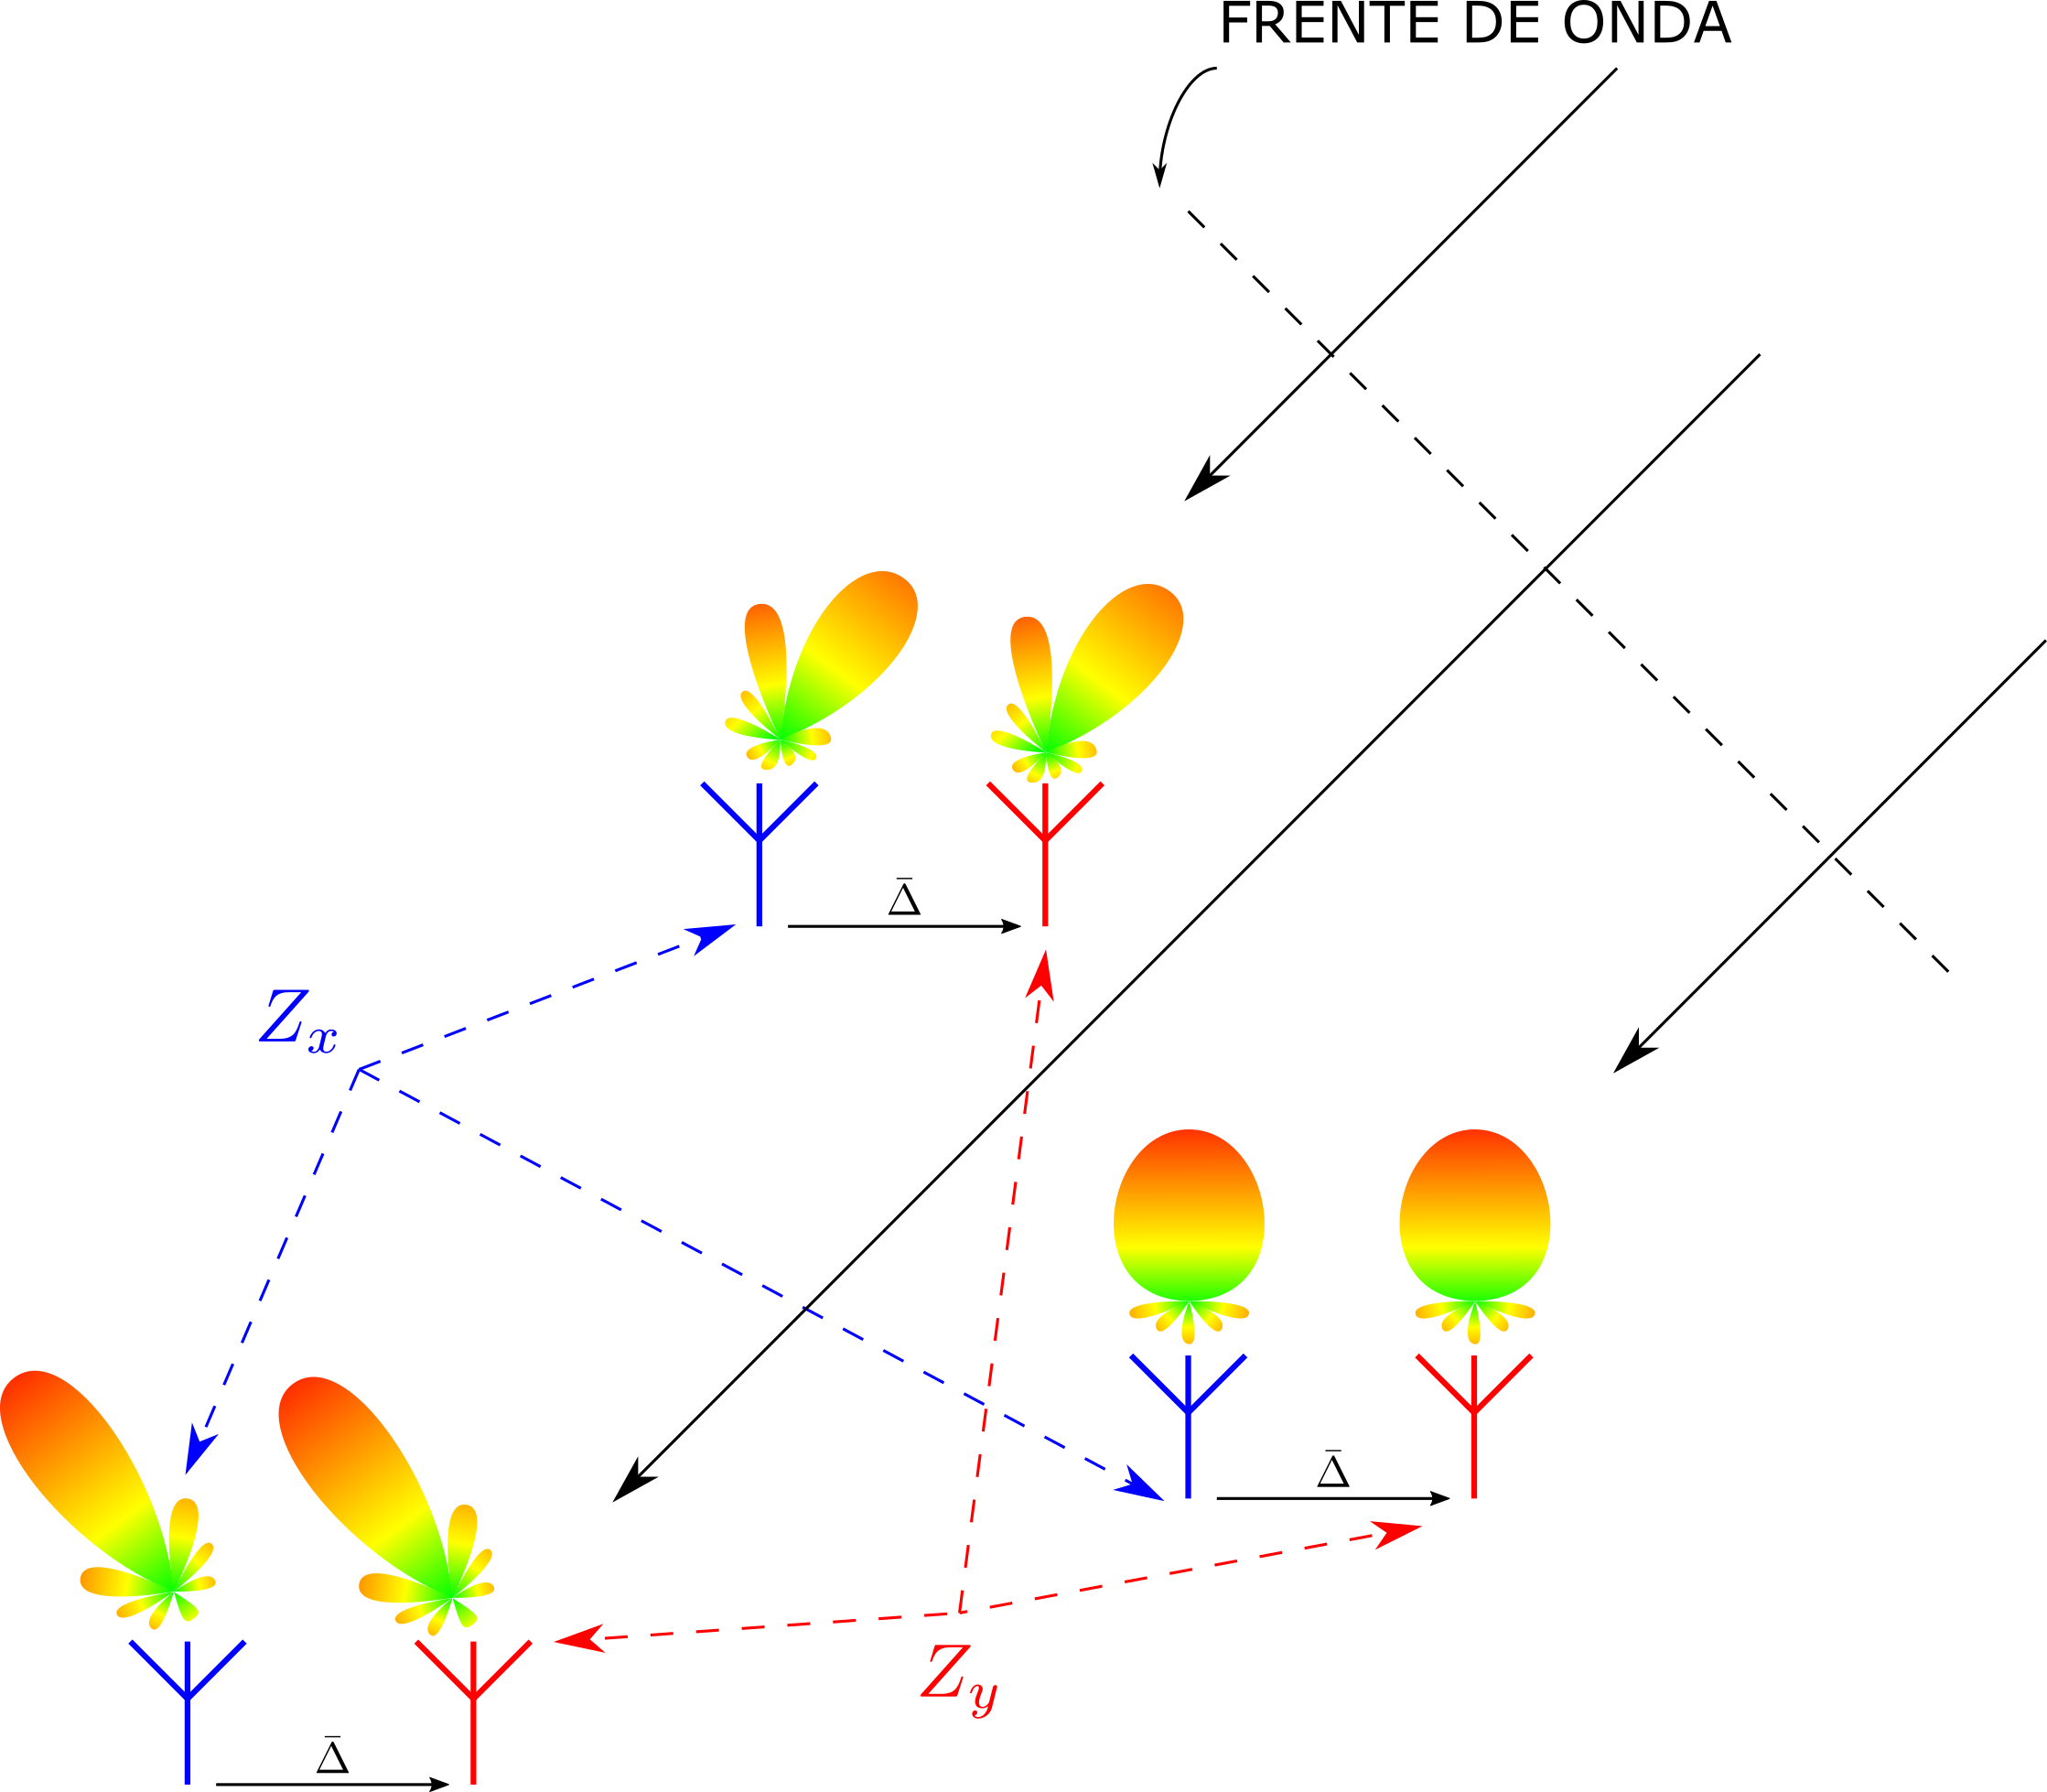
\includegraphics[width=0.7\linewidth]{images/03-DOAEst/esprit.png}
    \caption{Geometría del arreglo de antenas para el análisis del algoritmo ESPRIT. En azul y en rojo se separan los elementos pertenecientes a los subarreglos $Z_x$ y $Z_y$, respectivamente.}
    \label{fig:doaest_esprit_geometry}
\end{figure}

Bajo esta geometría, se puede considerar que el arreglo está compuestos por dos subarreglos, identificados en la figura por los elementos azules y los elementos rojos, los cuales conforman los subarreglos $Z_x$ y $Z_y$, respectivamente. Estos subarreglos son idénticos entre sí, con la única diferencia de que uno está trasladado con respecto al otro por el vector $\bar{\Delta}$. Las señales recibidas por cada elemento del par $i$-ésimo pueden ser expresadas como:
\begin{equation}
    \begin{split}
        x_i(t)&=\sum_{d=0}^{D-1} a_i(\theta_d,\varphi_d)\cdot s_d(t) + w_{x,i}(t)\\
        y_i(t)&=\sum_{d=0}^{D-1} a_i(\theta_d,\varphi_d)\cdot e^{j\bar{k}\cdot\bar{\Delta}}\cdot s_d(t) + w_{y,i}(t),
    \end{split}
\end{equation}
siendo $x_i(t)$ la señal recibida por el elemento perteneciente al subarreglo $Z_x$ y dentro del $i$-ésimo par, $y_i(t)$ la señal recibida por el elemento perteneciente al subarreglo $Z_y$ dentro del $i$-ésimo par y $a_i(\theta_d,\varphi_d)$ el elemento del vector de apuntamiento que corresponde al elemento de referencia dentro del par correspondiente (en este caso el perteneciente a $Z_x$) para una dirección de arribo $(\theta_d,\varphi_d)$. La dirección del vector de traslación $\bar{\Delta}$ indica la dirección con respecto a la cual se podrá estimar el ángulo de arribo. Por ejemplo, si la traslación se realiza sobre el eje $x$, solo se podrán estimar ángulos de arribo con respecto a este eje. Como consecuencia de esto, en el caso de la estimación bidimensional con ángulos de elevación y azimut se deberá contar con dos vectores de traslación, uno en cada dimensión de interés.

Combinando las salidas de todos los elementos de cada subarreglo se pueden expresar a las señales recibidas como:
\begin{equation}
    \begin{split}
        \bar{x}(t)&=\mathbf{A}s(t)+\bar{w}_x(t),\\
        \bar{y}(t)&=\mathbf{A \Phi} s(t)+ \bar{w}_y(t),
    \end{split}
\end{equation}
donde $\mathbf{A}$ es la matriz de apuntamiento correspondiente al subarreglo $Z_x$ y $\mathbf{\Phi}$ una matriz diagonal de tamaño $D \times D$ cuyos elementos están conformados por los desfasajes producidos entre pares de elementos para los $D$ frentes de ondas recibidos, es decir:
\begin{equation}
    \mathbf{\Phi}= \begin{bmatrix}
        e^{j\bar{k}_0\cdot \bar{\Delta}} & 0                                & \cdots & 0                                    \\
        0                                & e^{j\bar{k}_1\cdot \bar{\Delta}} &        & \vdots                               \\
        \vdots                           &                                  & \ddots & \vdots                               \\
        0                                & \cdots                           & \cdots & e^{j\bar{k}_{D-1}\cdot \bar{\Delta}}
    \end{bmatrix}=\textrm{diag}\{\phi_0,\phi_1,...,\phi_{D-1}\}
\end{equation}
siendo $\phi_d=e^{j\bar{k}_d\cdot \bar{\Delta}}$ con $d=0,1,...,D-1$. La matriz $\mathbf{\Phi}$ recibe el nombre de \emph{operador de rotación de subespacio} \cite{bib:esprit_roy}.
Si se define al número de pares de elementos como $M$, de manera tal que el número de elementos sea $2M$, y al vector de salida del arreglo entero como $\bar{z}(t)$ podemos escribirlo como:
\begin{gather}
    \bar{z}(t)=\begin{bmatrix}
        \bar{x}(t) \\
        \bar{y}(t)
    \end{bmatrix}
    = \bar{\mathbf{A}} s(t) + \bar{w}(t),\\
    \bar{\mathbf{A}}=\begin{bmatrix}
        \mathbf{A} \\
        \mathbf{A\Phi}
    \end{bmatrix}_{(2M \times D)},
    \quad
    \bar{w}(t)=\begin{bmatrix}
        \bar{w}_x \\
        \bar{w}_y
    \end{bmatrix}_{(2M \times 1)}\nonumber
\end{gather}

Una consideración a tener en cuenta para el resto del análisis es que $D$ tiene que ser menor a $M$, aunque posteriormente se mostrará que en realidad $D$ puede ser como máximo menor a la cantidad total de elementos en el arreglo.

Los vectores de $\bar{\mathbf{A}}$ generan el subespacio de señal. Si se define la matriz $\mathbf{Z}$ como la matriz conformada por los vectores obtenidos luego de muestrear $N$ veces a todos los elementos del arreglo de antenas podemos expresarla de la siguiente manera:
\begin{equation}
    Z=\begin{bmatrix}
        \bar{z}_0 & \bar{z}_1 & \cdots & \bar{z}_{N-1}
        \label{eq:doaest_esprit_z}
    \end{bmatrix}_{(2M\times N)},
\end{equation}
donde $\bar{z}_n$ con $n=0,1,...,N-1$ es el vector de muestras tomadas en el instante $n$.
Si se aplica la descomposición en subespacio de ruido y señal de las muestras contenidas en la matriz $\mathbf{Z}$, como se mostró en la Sección \ref{subc:doaest_datamodel}, puede verse que la matriz $\mathbf{E_S}$ genera el mismo espacio $2M$-dimensional que los vectores de $\bar{\mathbf{A}}$, ya que ambos generan el subespacio de señal. En consecuencia, debe existir una matriz de transformación invertible $\mathbf{T}$ que mapee elementos de $\mathbf{E_S}$ a $\bar{\mathbf{A}}$, es decir, existe $\mathbf{T}$ tal que:
\begin{equation}
    \mathbf{E_S}=\bar{\mathbf{A}}\mathbf{T}
\end{equation}

Debido a esto la matriz $\mathbf{E_S}$ puede descomponerse en dos submatrices $\mathbf{E_X}$ y $\mathbf{E_Y}$ de tamaño $M\times D$ de manera tal que:
\begin{equation}
    \mathbf{E_S}=\begin{bmatrix}
        \mathbf{E_X} \\
        \mathbf{E_Y}
    \end{bmatrix}=
    \begin{bmatrix}
        \mathbf{AT} \\
        \mathbf{A\Phi T}
    \end{bmatrix}
    \label{eq:doaest_esprit_ex_ey}
\end{equation}
de donde puede verse que
\begin{equation}
    \textrm{Span}\{\mathbf{E_X}\}=\textrm{Span}\{\mathbf{E_Y}\}=\textrm{Span}\{\mathbf{A}\}
\end{equation}
(donde $\textrm{Span}\{\mathbf{V}\}$ es el subespacio generado por $\mathbf{V}$), debido a que la rotación aplicada por $\mathbf{\Phi}$ no modifica el subespacio generado \cite{bib:esprit_roy}.
Ahora se define la matriz $\mathbf{E_{XY}}$ como:
\begin{equation}
    \mathbf{E_{XY}}:= [\mathbf{E_{X}} | \mathbf{E_{Y}}],
    \label{eq:doaest_e_xy}
\end{equation}
la cual tiene rango $D$ debido a que $\mathbf{E_{X}}$ y $\mathbf{E_{Y}}$ tienen el mismo espacio de columnas. Debido a esto, debe existir una matriz $\mathbf{K} \in \mathbb{C}^{(2D\times D)}$ tal que:
\begin{align}
    \mathbf{0} & = \mathbf{E_{XY}K} = \mathbf{E_X K_X} + \mathbf{E_Y K_Y} \label{eq:doaest_kx_ky} \\
               & = \mathbf{ATK_X+A\Phi T K_Y},
    \label{eq:doaest_kernel}
\end{align}
\begin{equation*}
    \mathbf{K}=\begin{bmatrix}
        \mathbf{K_X} \\
        \mathbf{K_Y}
    \end{bmatrix},
\end{equation*}
es decir que $\mathbf{K}$ genera el núcleo de $\mathbf{E_{XY}}$. A partir de la Ecuación \ref{eq:doaest_kx_ky} puede escribirse:
\begin{align}
    -\mathbf{E_X K_X}                                  & =\mathbf{E_Y K_Y}\nonumber \\
    \mathbf{E_X} \left( \mathbf{-K_X K_Y}^{-1} \right) & =\mathbf{E_Y}\nonumber     \\
    \mathbf{E_X \Psi}                                  & =\mathbf{E_Y}
    \label{eq:doaest_psi}
\end{align}
siendo $\mathbf{\Psi}:=-\mathbf{K_X K_Y}^{-1}$ la matriz de transformación de $\mathbf{E_X}$ a $\mathbf{E_Y}$. A partir de esta definición se puede reescribir la Ecuación \ref{eq:doaest_kernel} de la siguiente manera:
\begin{equation}
    \mathbf{AT\Psi} = \mathbf{A\Phi T \rightarrow \mathbf{AT\Psi T}^{-1} = \mathbf{A\Phi}}
\end{equation}

Suponiendo que $\mathbf{A}$ es de rango completo se puede escribir:
\begin{equation}
    \mathbf{T\Psi T}^{-1} = \mathbf{\Phi},
\end{equation}
por ende, los autovalores de $\mathbf{\Psi}$ son los elementos de la diagonal de $\mathbf{\Phi}$, y los vectores de $\mathbf{T}$ son los autovectores de $\mathbf{\Phi}$. Debido a esto, obteniendo una estimación de $\mathbf{\Psi}$ se puede obtener una estimación de la matriz $\mathbf{\Phi}$ y a partir de ahí los ángulos de arribo.

Los subarreglos no tienen por qué ser conjuntos disjuntos, la posibilidad de armar subarreglos con elementos en común está permitida en el algoritmo ESPRIT y es una técnica que permite reducir la cantidad de elementos necesaria para poder implementarlo. Si contamos con un arreglo de antenas en fase de geometría ARU se deberá aplicar el algoritmo ESPRIT en dos dimensiones distintas para obtener los ángulos de elevación y azimut de la dirección de arribo. La opción lógica es elegir subarreglos separados en el eje $x$ y en el eje $y$, como se muestra en la Figura \ref{fig:doaest_esprit2d}.
\begin{figure}[ht!]
    \centering
    \begin{subfigure}[b]{0.49\textwidth}
        \centering
        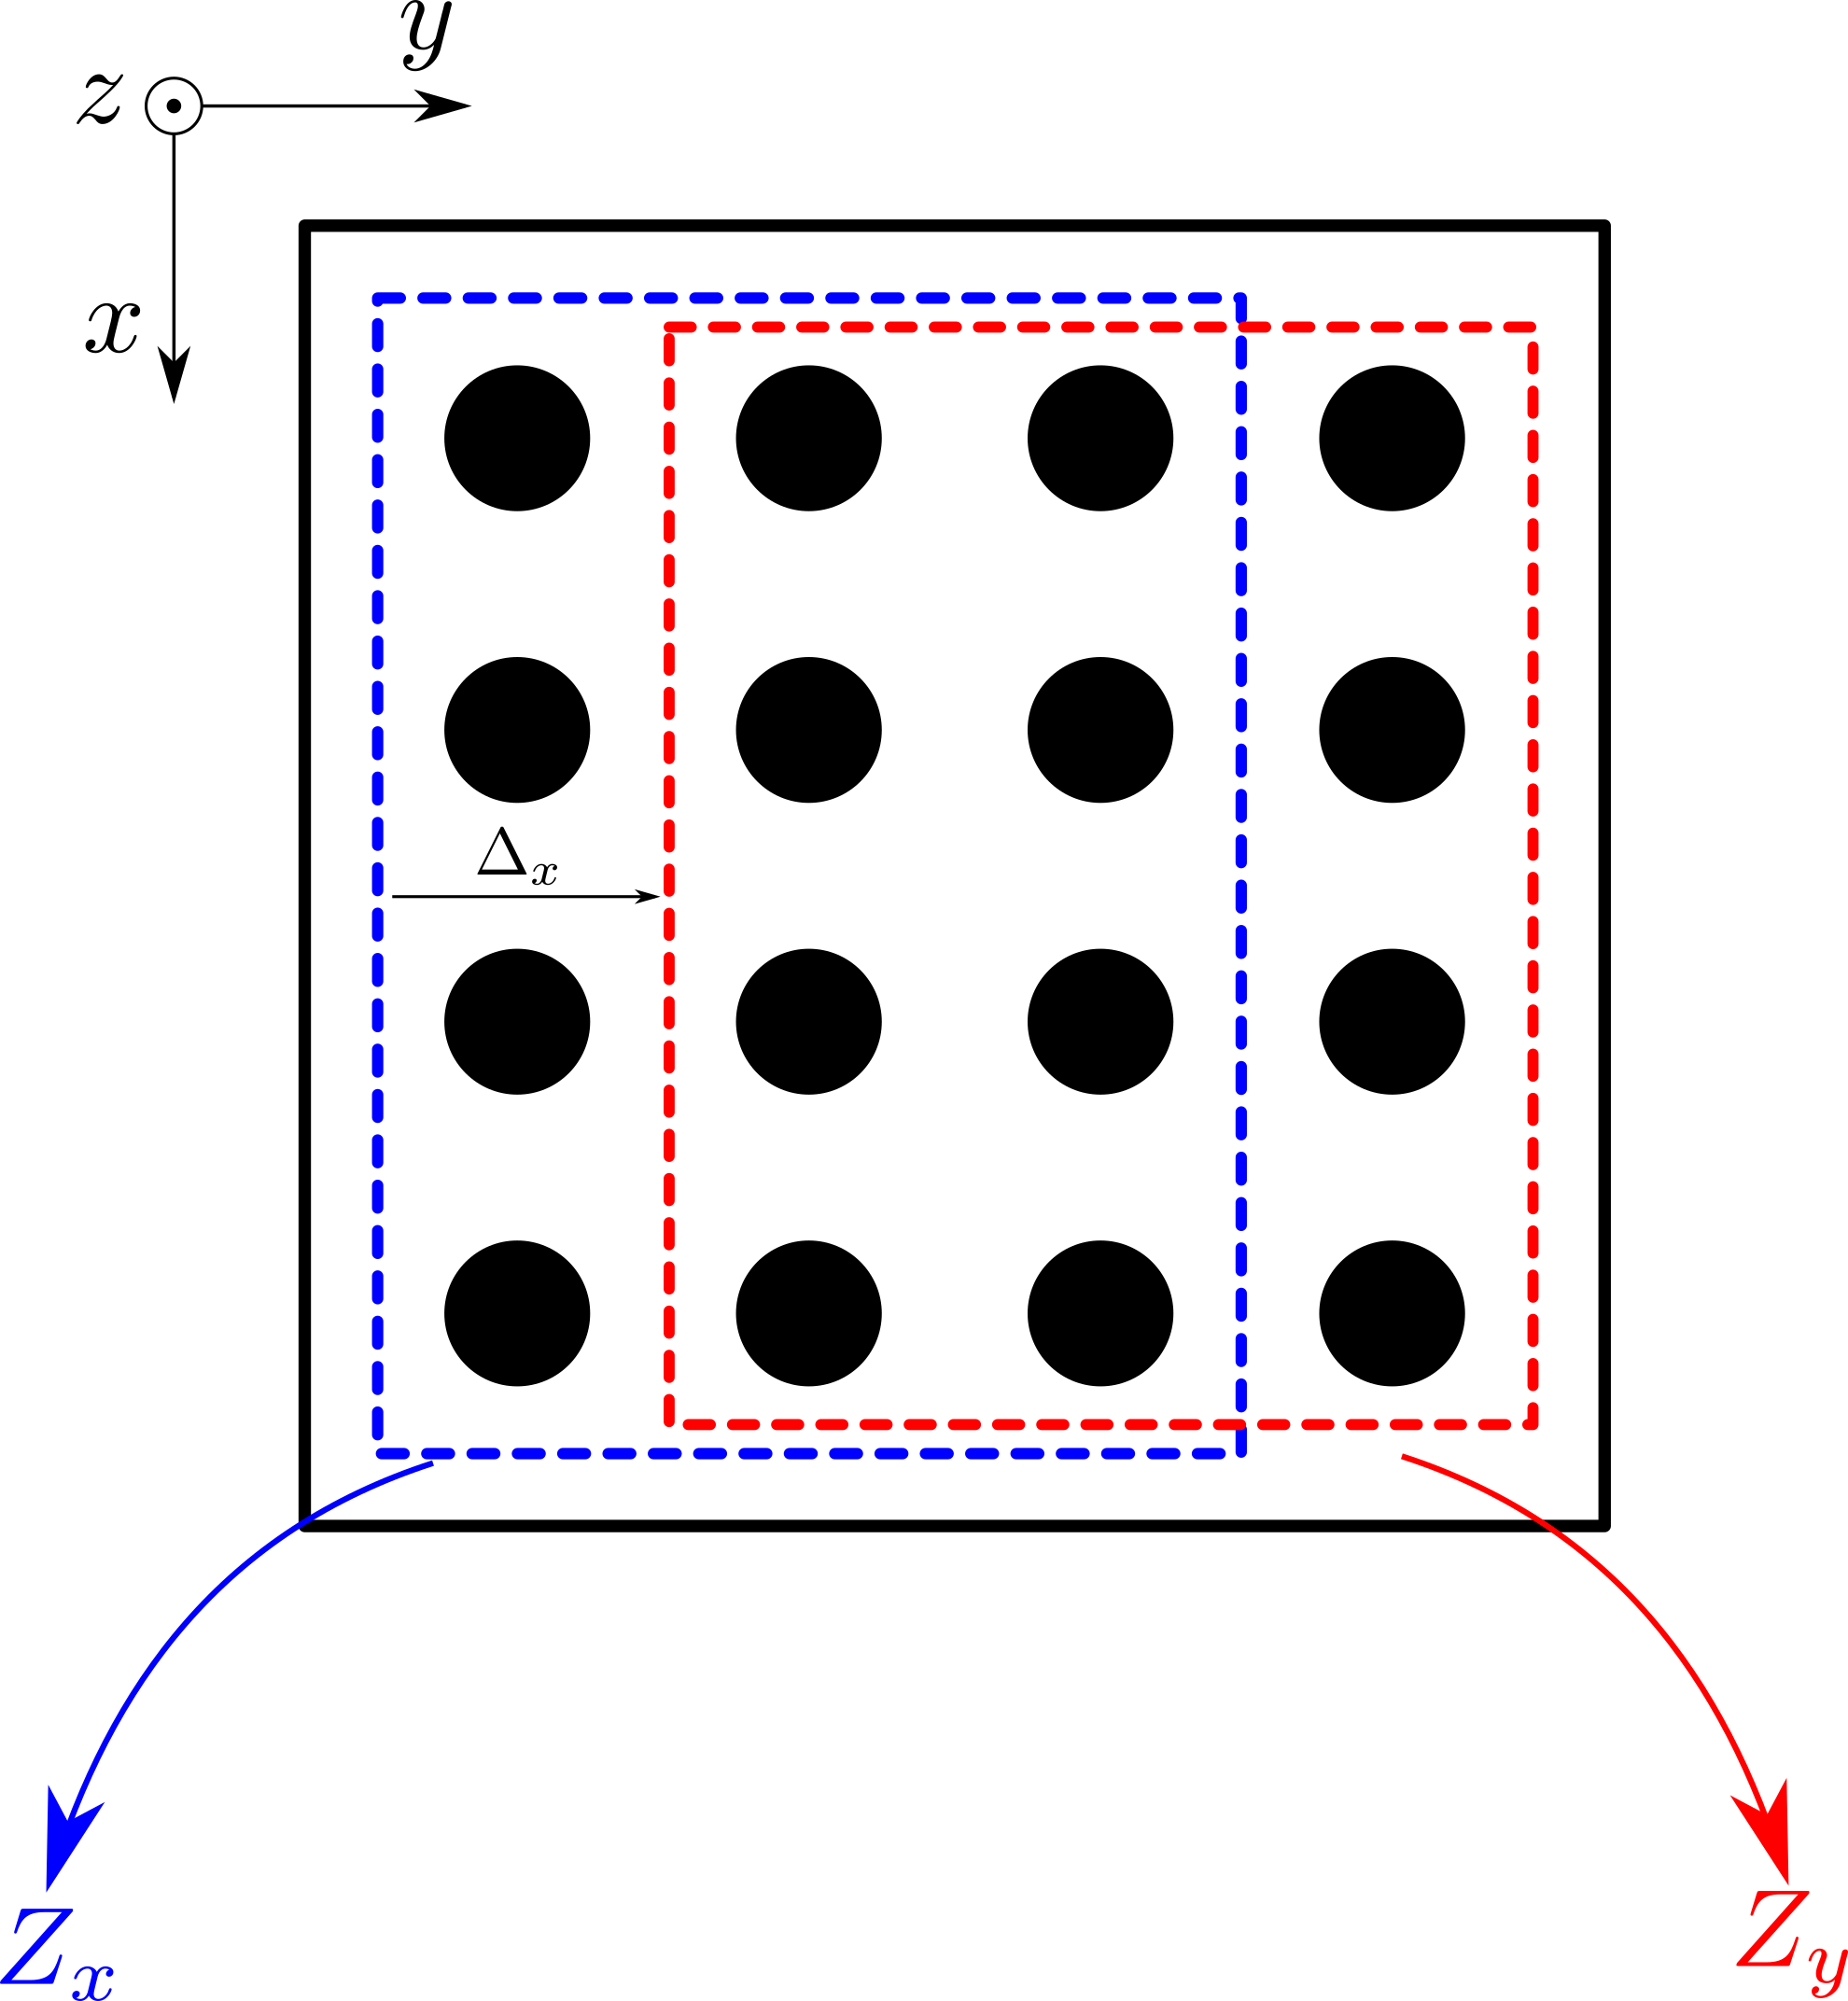
\includegraphics[width=\linewidth]{images/03-DOAEst/esprit_x.png}
    \end{subfigure}
    \hfill
    \begin{subfigure}[b]{0.49\textwidth}
        \centering
        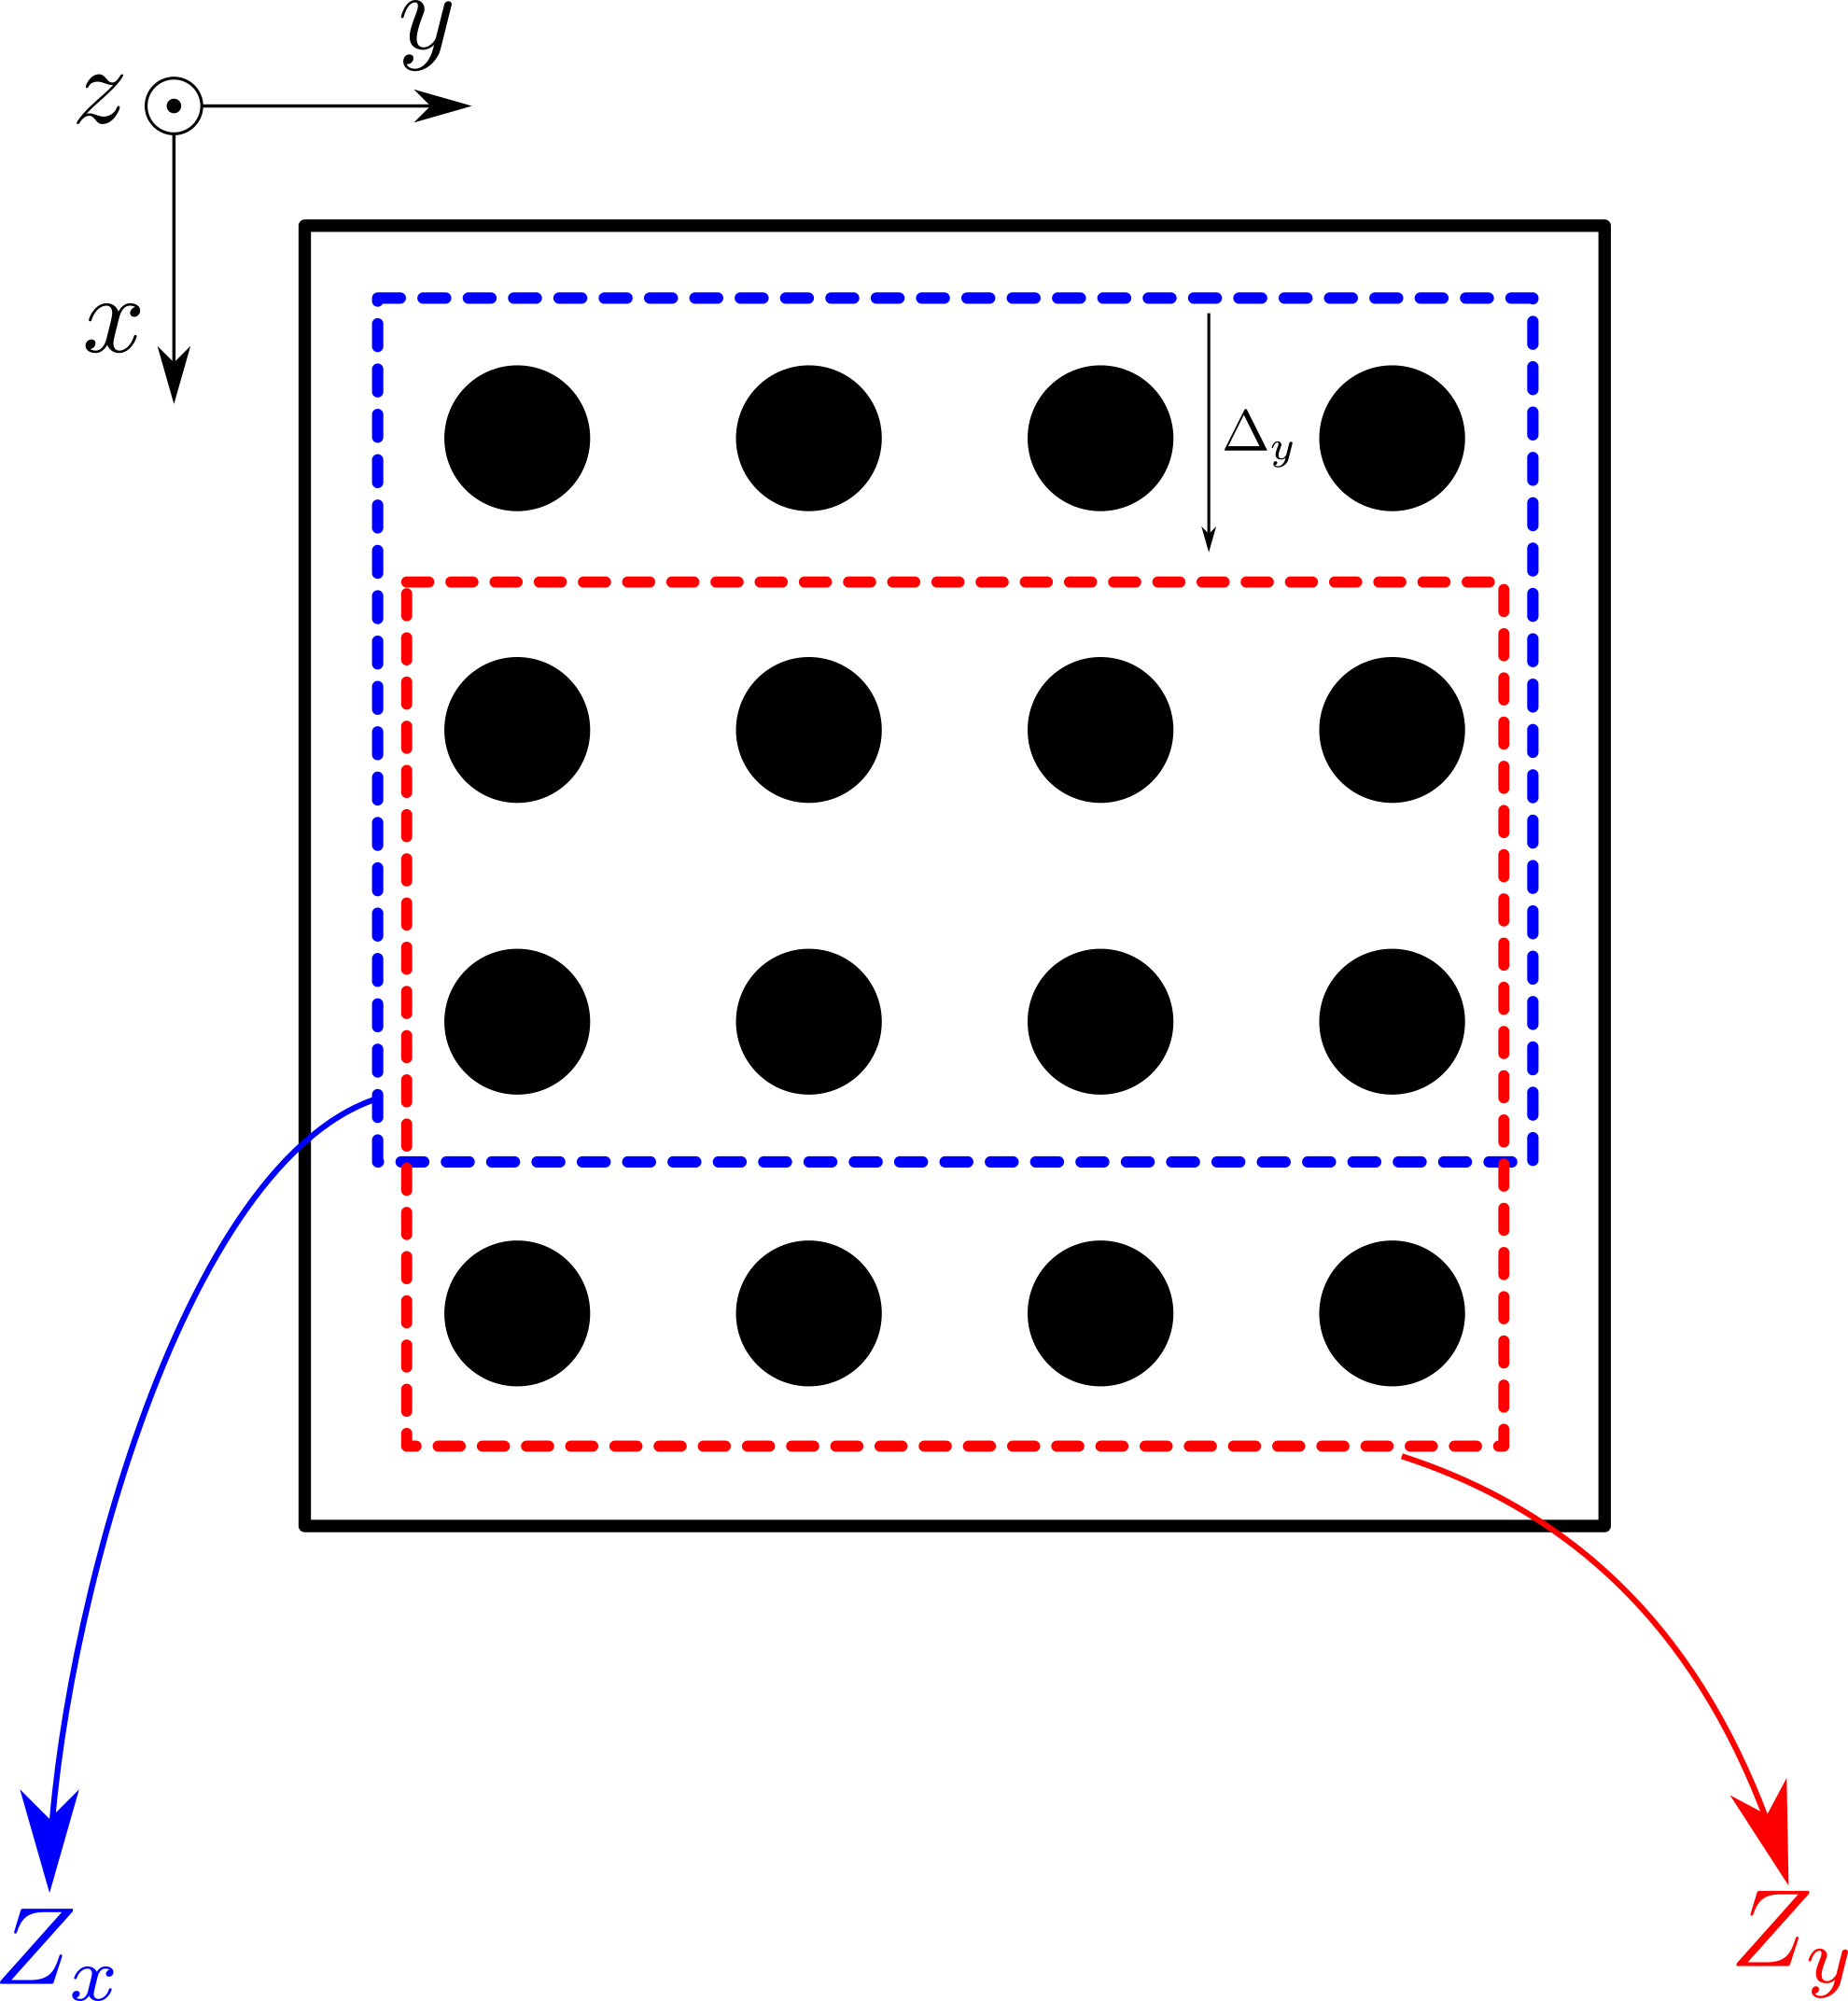
\includegraphics[width=\linewidth]{images/03-DOAEst/esprit_y.png}
    \end{subfigure}
    \caption{Una posible elección de subarreglos para la aplicación del algoritmo ESPRIT en dos dimensiones utilizando un ARU.}
    \label{fig:doaest_esprit2d}
\end{figure}

Teniendo una geometría como la mostrada, luego de utilizar ESPRIT en las dos dimensiones indicadas se obtendrán dos matrices $\mathbf{\Phi_x}$ y $\mathbf{\Phi_y}$ de tamaño $D\times 1$, los cuales permiten obtener los ángulos de arribo haciendo:
\begin{gather}
    \theta_d=\arccos\left( \sqrt{\frac{(\angle{\phi_{x,d}})^2+(\angle{\phi_{y,d}})^2 }{(k\cdot \delta)^2}},\label{eq:doaest_thetaesprit}\right)\\
    \varphi_d=\arctan2\left(\frac{\angle{\phi_{y,d}}}{\angle{\phi_{x,d}}} \right)\label{eq:doaest_phiesprit}
\end{gather}
con $d=0,1,...,D-1$ y siendo $\delta$ la separación entre elementos. La deducción de estas expresiones se muestra en el Apéndice \ref{AP:esprit_angles}.

\subsubsection{Estimación del operador de rotación de subespacio}
Al igual que como ocurre en MUSIC, al no poder operar en la práctica con infinitas muestras, la matriz $\mathbf{E_S}$ obtenida mediante SVD aplicada a la matriz $\mathbf{Z}$ o por descomposición en autovalores de la estimación de la matriz de covarianza $\mathbf{\hat{R}_{ZZ}}$ no es la teórica, sino una estimación de ella, la cual se denota como $\mathbf{\hat{E}_S}$. Por ende, $\mathbf{\hat{E}_S}$ no genera el subespacio de señal y $\textrm{Span}\{ \mathbf{\hat{E}_S} \}\neq \textrm{Span}\{ \mathbf{\bar{A}} \}$. Además $\textrm{Span}\{ \mathbf{\hat{E}_X} \}\neq \textrm{Span}\{ \mathbf{\hat{E}_Y} \}$, y debido a esto la matriz $\mathbf{\Psi}$ no puede encontrarse de la manera que se mostró en la Ecuación \ref{eq:doaest_psi}. Es por esto que debe elegirse un criterio para obtener una correcta estimación de $\mathbf{\hat{\Psi}}$ para luego estimar $\mathbf{\hat{\Phi}}$, y ese criterio es el de \emph{mínimos cuadrados totales} (\emph{TLS} por sus siglas en inglés). Este criterio consiste en reemplazar la matriz nula en la Ecuación \ref{eq:doaest_kx_ky} por una matriz de errores cuya norma de Frobenius debe minimizarse \cite{bib:esprit_roy}. La solución a este problema primero consiste en calcular la SVD de la matriz $\mathbf{\hat{E}_{XY}}$ definida en la Ecuación \ref{eq:doaest_e_xy}:
\begin{equation}
    \mathbf{\hat{E}_{XY}} = \mathbf{U\Sigma V}
\end{equation}

A partir de esto se trabaja con la matriz $\mathbf{V}\in \mathbb{C}^{2D\times 2D}$, la cual se particiona en 4 matrices de tamaño $D \times D$ de la siguiente manera:
\begin{equation}
    \mathbf{V} = \begin{bmatrix}
        \mathbf{V_{00}} & \mathbf{V_{01}} \\
        \mathbf{V_{10}} & \mathbf{V_{11}}
    \end{bmatrix}
    \label{eq:doaest_v_part}
\end{equation}

Luego la solución TLS viene dada por:
\begin{equation}
    \mathbf{\hat{\Psi}_{TLS}}= -\mathbf{V_{01}}\mathbf{V_{11}}^{-1}
    \label{eq:doaest_psi_tls}
\end{equation}
cuyos autovalores representan a los elementos $\hat{\phi}_d$ con $d=0,1,...,D-1$ de la matriz $\mathbf{\hat{\Phi}}$.

Finalmente, la dirección de arribo estimada $(\hat{\theta_d},\hat{\phi_d})$ se obtiene mediante las Ecuaciones \ref{eq:doaest_thetaesprit} y \ref{eq:doaest_phiesprit}.

\subsection{Algoritmo}\label{subc:doaest_esprit_alg}
A continuación se detallan los pasos para implementar el algoritmo ESPRIT:
\begin{enumerate}
    \item Separar el arreglo de antenas en dos subarreglos iguales pero trasladados por un vector $\bar{\Delta}$ uno del otro.
    \item Formar la matriz $\mathbf{Z}$ definida en la Ecuación \ref{eq:doaest_esprit_z} utilizando varias muestras temporales.
    \item Realizar la descomposición en autovalores de la matriz $\mathbf{\hat{R}_{ZZ}}$ obtenida con la Ecuación \ref{eq:doaest_rxx_est} o realizar la SVD sobre la matriz $\mathbf{Z}$ quedándose únicamente con los valores singulares y los vectores singulares izquierdos $\mathbf{U}$.
    \item Estimar el número $\hat{D}$ de señales recibidas. Las técnicas para lograr esto se mencionan en el Capítulo \ref{ch:machinelearning}.
    \item Elegir los $\hat{D}$ autovectores de la descomposición de $\mathbf{\hat{R}_{ZZ}}$ correspondientes a los autovalores más grandes, o los vectores singulares de $\mathbf{U}$ correspondientes a los valores singulares más grandes de la SVD de $\mathbf{Z}$ para formar la matriz $\mathbf{\hat{E}_S}$ como se indica en la Ecuación \ref{eq:doaest_es_en}.
    \item Separar la matriz $\mathbf{\hat{E}_S}$ en $\mathbf{\hat{E}_X}$ y $\mathbf{\hat{E}_Y}$ como se muestra en la Ecuación \ref{eq:doaest_esprit_ex_ey}.
    \item Armar la matriz $\mathbf{\hat{E}_{XY}}$ como se muestra en la Ecuación \ref{eq:doaest_e_xy} y obtener su SVD quedándose únicamente con los vectores singulares derechos $\mathbf{V}$.
    \item Particionar la matriz $\mathbf{V}$ en 4 submatrices de tamaño $D\times D$ como se muestra en la Ecuación \ref{eq:doaest_v_part}.
    \item Obtener $\mathbf{\hat{\Psi}_{TLS}}$ como se indica en la Ecuación \ref{eq:doaest_psi_tls}.
    \item Obtener los elementos de la matriz $\mathbf{\hat{\Phi}}$ obteniendo los autovalores de $\mathbf{\hat{\Psi}_{TLS}}$.
    \item Obtener los ángulos de arribo $(\hat{\theta_d},\hat{\phi_d})$ a partir de las Ecuaciones \ref{eq:doaest_thetaesprit} y \ref{eq:doaest_phiesprit}.
\end{enumerate}

\section{Simulaciones}\label{subc:doaest_comparaciones}
Utilizando el modelo de muestras que se detalló en la Sección \ref{subc:doaest_datamodel} y los algoritmos descriptos en las Secciones \ref{subc:doaest_music_alg} y \ref{subc:doaest_esprit_alg}, se implementaron ambas técnicas de estimación de dirección de arribo, comparándolas con respecto al error obtenido en la estimación y el tiempo de ejecución de cada una.
En todas las simulaciones realizadas a continuación se utilizó el método de descomposición en valores singulares para la obtención de los estimadores de subespacios de señal y ruido, y no se realizó la estimación de cantidad de señales arribantes, fijando este número en 1. Además, en ambos algoritmos se utilizó una técnica de muestreo aleatorio para mejorar la eficiencia en las estimaciones, la cual se detalla en el Capítulo \ref{ch:randomsampling}. Finalmente, se consideró que el arreglo de antenas es de tipo ARU de tamaño $M_x \times M_y$ y que la separación entre elementos es de media longitud de onda de la portadora.
Para generar las muestras simuladas se desarrolló un algoritmo que a partir de una muestra de una señal generaba el vector de muestras correspondientes a cada elemento del arreglo, simulando el comportamiento de la señal llegando al mismo con una determinada DOA según el análisis descripto en la Sección \ref{subc:beamforming_phasedarraystipos} para el caso de un arreglo rectangular uniforme. Como señal de prueba se utilizó la captura de un beacon del satélite GOMX-1 \cite{bib:gomx-1}.

En esta sección se utilizarán los siguientes símbolos para identificar a los parámetros de las simulaciones realizadas:
\begin{itemize}
    \item $M_x$: número de elementos del ARU en la dirección $x$.
    \item $M_y$: número de elementos del ARU en la dirección $y$.
    \item $M$: número total de elementos en el ARU.
    \item $\mathfrak{R}_{\textrm{MUSIC}}$: resolución del dominio de búsqueda del algoritmo MUSIC tanto en azimut como en elevación.
    \item $N$: número de vectores de muestras con los que se alimentó a cada algoritmo.
    \item $\frac{\sigma_d}{d}$: error relativo en la separación de elementos con respecto a la distancia nominal $d$.
\end{itemize}

La definición de SNR utilizada para todas las simulaciones es la siguiente:
\begin{equation}
    \mathrm{SNR}=\frac{\mathbf{E}\{|s[n]|^2\}}{\mathbf{E}\{|w[n]|^2\}}
\end{equation}

La plataforma de cómputo donde se realizaron todas las simulaciones es una computadora portátil Alienware 17 R3 con las siguientes especificaciones:
\begin{itemize}
    \item Microprocesador: Intel\textsuperscript{\textregistered} Core\textsuperscript{\texttrademark} i7-6700HQ CPU @ 2,60 GHz.
    \item Memoria RAM: 32 GB.
    \item Sistema operativo: Windows 10 (64 bits).
\end{itemize}

Además, los programas de las simulaciones fueron desarrollados utilizando el lenguaje \texttt{Python} en su versión 3.8.5.

\subsection{RMSE vs. SNR}\label{subc:doaest_error_vs_snr}

Para realizar esta simulación se promediaron 10 realizaciones por cada valor de SNR. En cada realización se alteraba aleatoriamente la DOA y las muestras elegidas por el algoritmo de muestreo aleatorio. Para el caso del algoritmo MUSIC, el dominio de búsqueda se generó de manera tal de poder contar con una resolución en la estimación de $\mathfrak{R}_{\textrm{MUSIC}}=0,5\grad$ tanto en elevación como en azimut. La métrica de error utilizada en este análisis es la raíz cuadrada del error cuadrático medio (RMSE), la cual se obtiene de la siguiente manera:
\begin{equation}
    \textrm{RMSE}(\hat{\theta},\hat{\varphi})=\sqrt{\frac{1}{N}\sum^{N-1}_{i=0}\left( \left(\hat{\theta_i}-\theta_i \right)^2 + \left(\hat{\varphi_i}-\varphi_i \right)^2\right)}
\end{equation}
siendo $N$ el número de realizaciones.
Los parámetros utilizados en esta simulación son:
\begin{itemize}
    \item $M_x = 4$
    \item $M_y = 4$
    \item $N = 1500$ vectores de muestras
    \item $\frac{\sigma_d}{d}=0$
    \item $\mathfrak{R}_{\textrm{MUSIC}}=0,5\grad$
\end{itemize}

Los resultados obtenidos se muestran en la Figura \ref{fig:doaest_error_vs_snr}.
\begin{figure}[ht!]
    \centering
    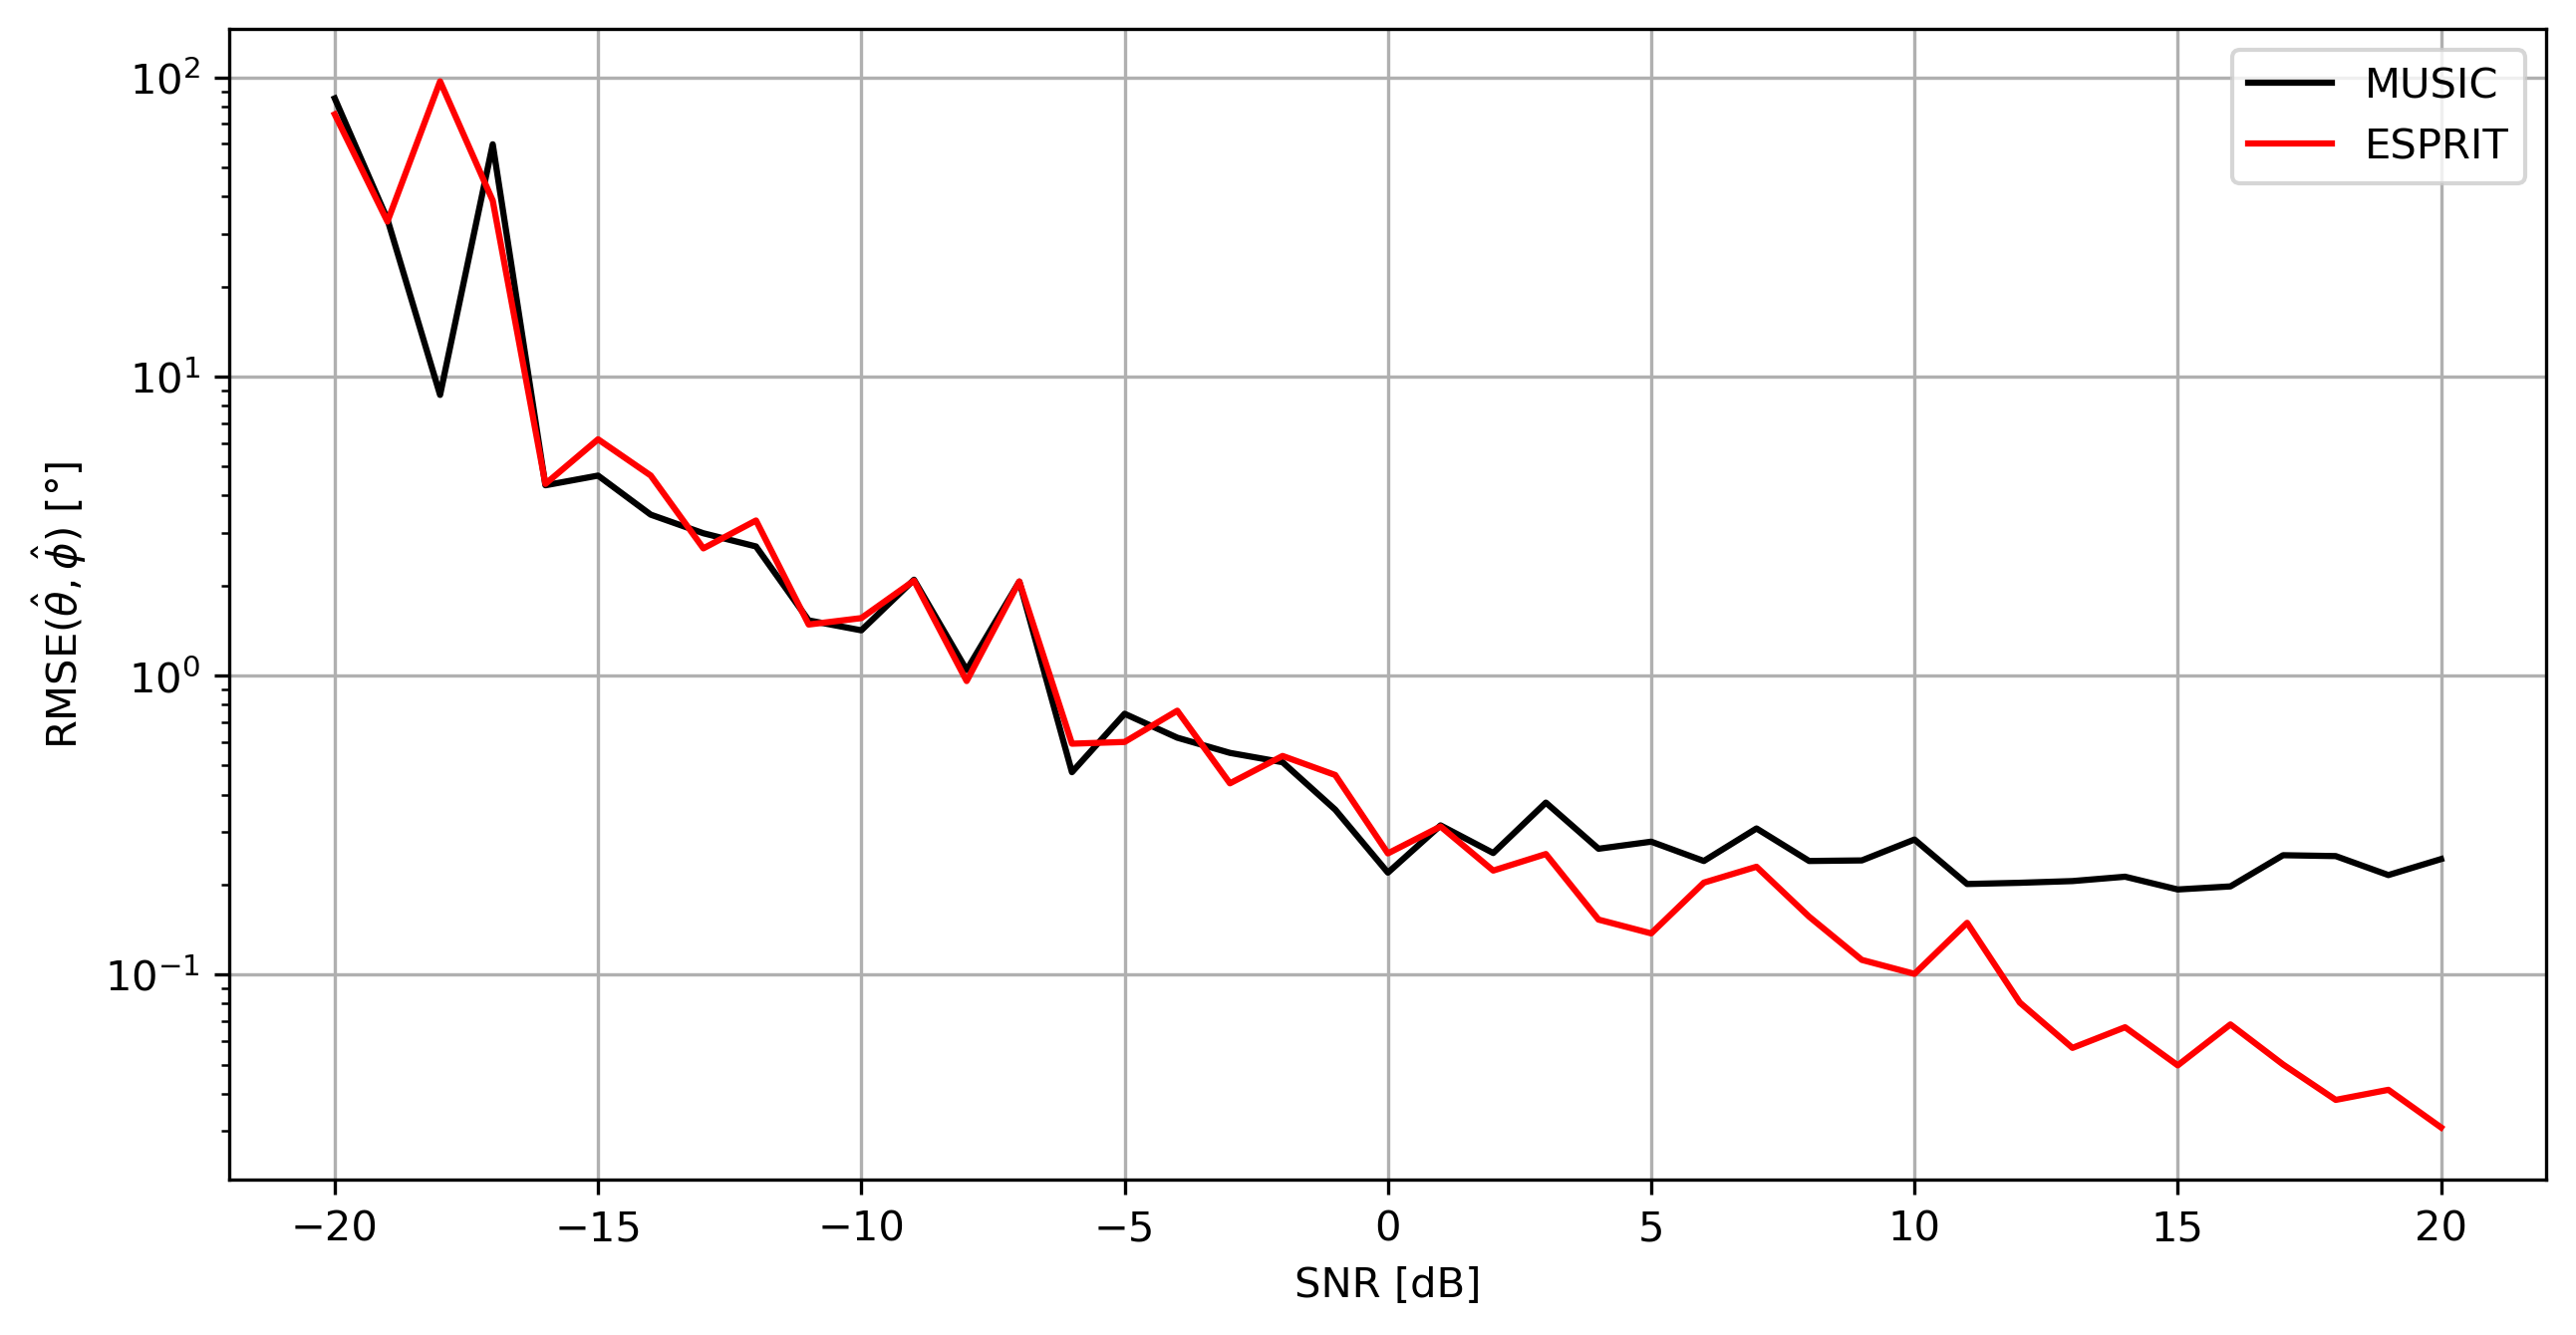
\includegraphics[width=0.9\linewidth]{images/03-DOAEst/error_vs_snr.png}
    \caption{Gráfico de comparación del RMSE en función de la SNR para los algoritmos MUSIC y ESPRIT.}
    \label{fig:doaest_error_vs_snr}
\end{figure}

Como puede apreciarse, ambos algoritmos se desempeñan de manera similar en el rango de SNR evaluado, alcanzando errores menores al grado para valores de SNR a partir de -5 dB. También se puede ver que, para valores de SNR mayores a 0 dB, MUSIC comienza a verse limitado por su resolución (la cual puede mejorarse a costa de un mayor requerimiento de procesamiento), y ESPRIT continúa mejorando la estimación alcanzando errores menores a $0,1\grad$.

Como dato adicional en la Figura \ref{fig:doaest_p_mu} se muestra cómo varía el pseudoespectro de MUSIC para el caso de una señal arribando con una DOA $(\theta = 45\grad, \varphi=30\grad)$ para distintos valores de SNR.
\begin{figure}[ht!]
    \centering
    \begin{subfigure}[b]{0.49\textwidth}
        \centering
        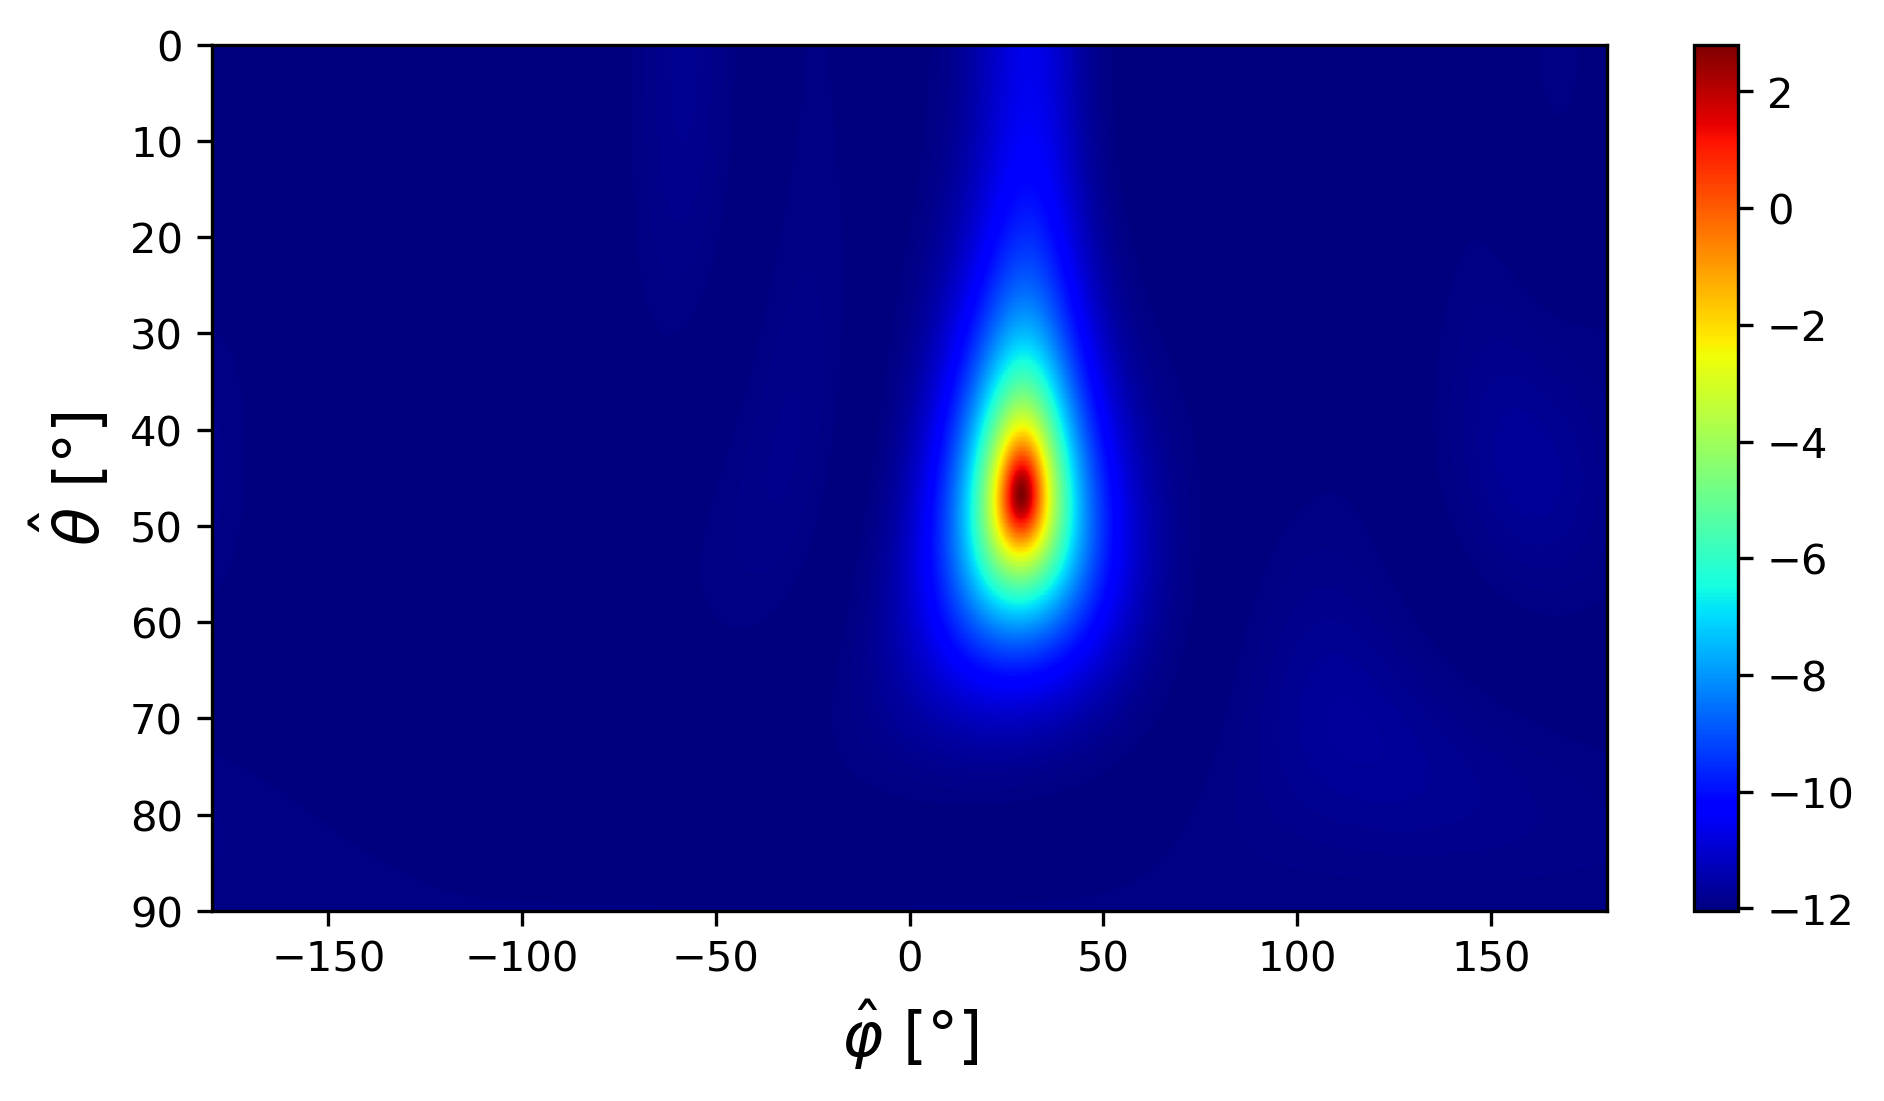
\includegraphics[width=\linewidth]{images/03-DOAEst/p_mu_-10.png}
        \caption{SNR = -10 dB}
    \end{subfigure}
    \hfill
    \begin{subfigure}[b]{0.49\textwidth}
        \centering
        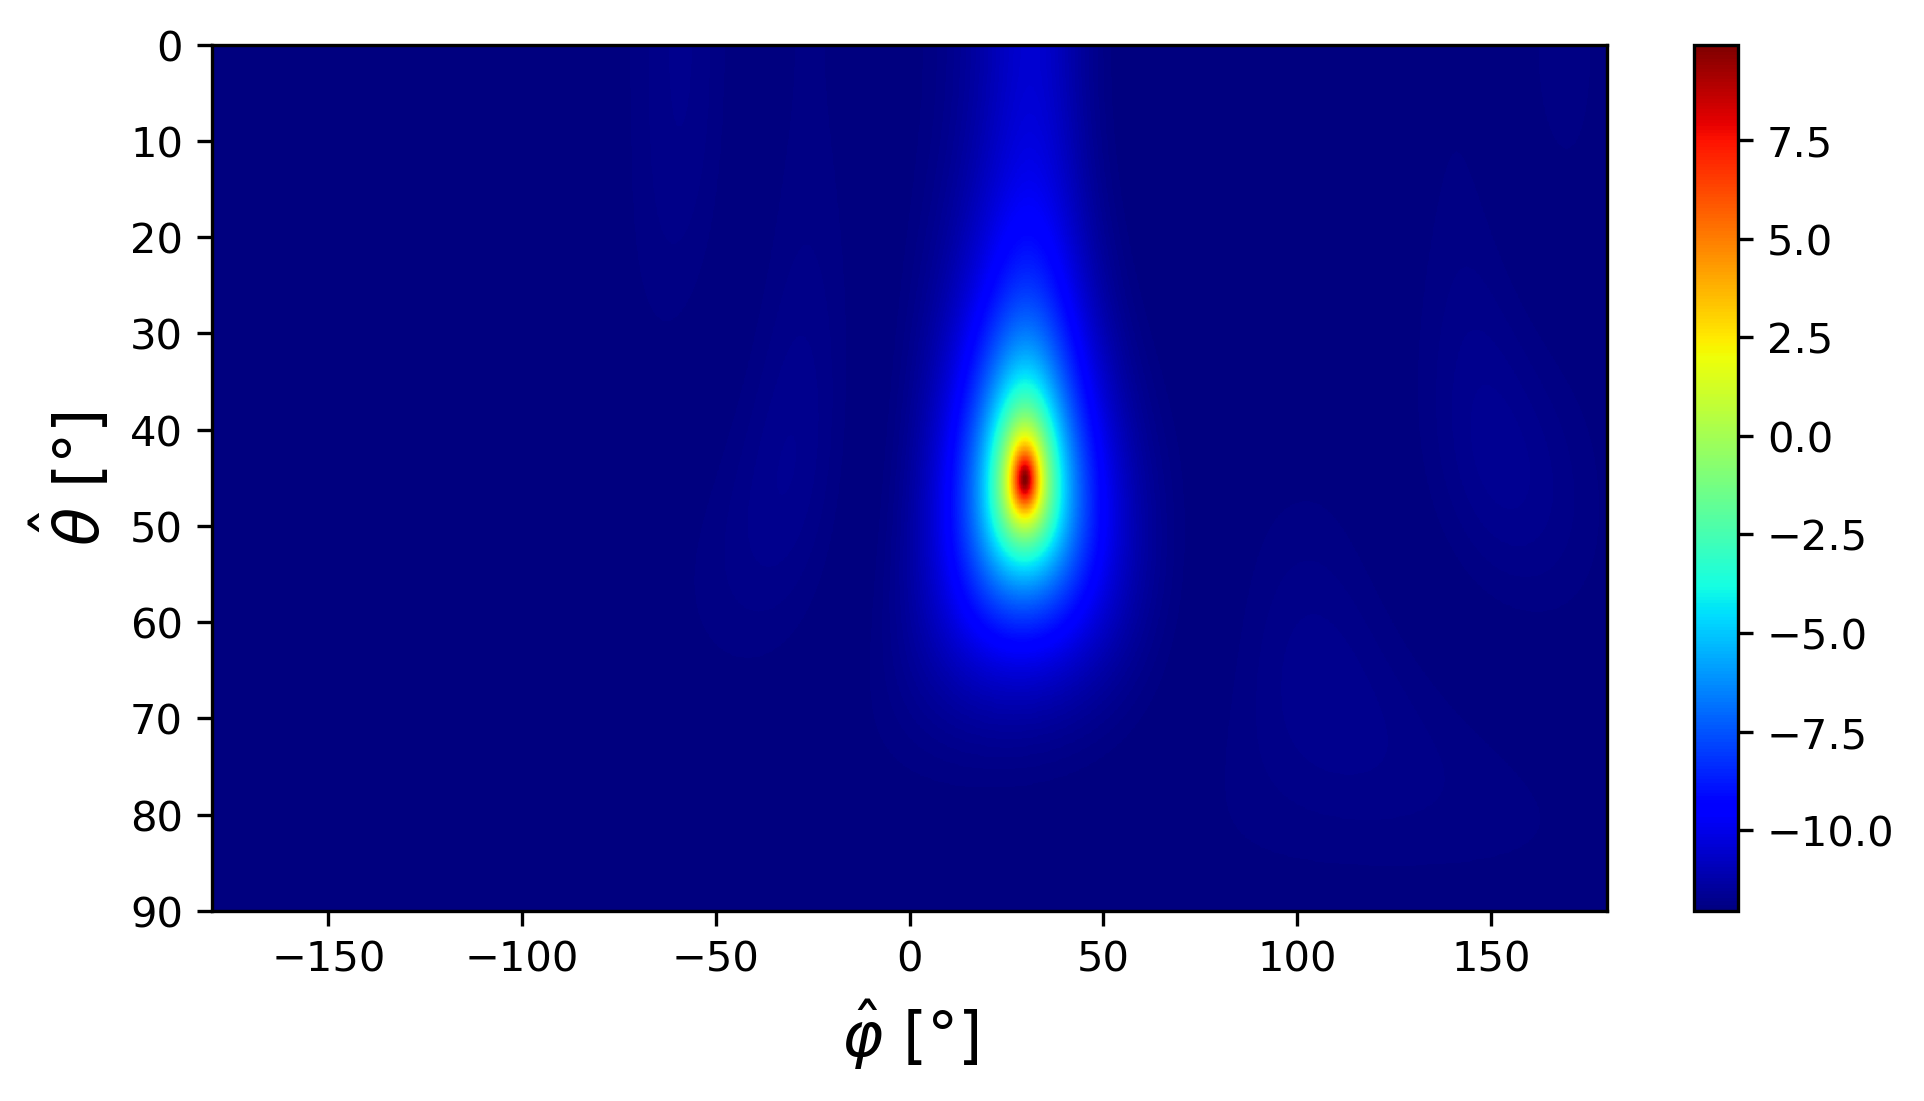
\includegraphics[width=\linewidth]{images/03-DOAEst/p_mu_-5.png}
        \caption{SNR = -5 dB}
    \end{subfigure}
    \hfill
    \begin{subfigure}[b]{0.49\textwidth}
        \centering
        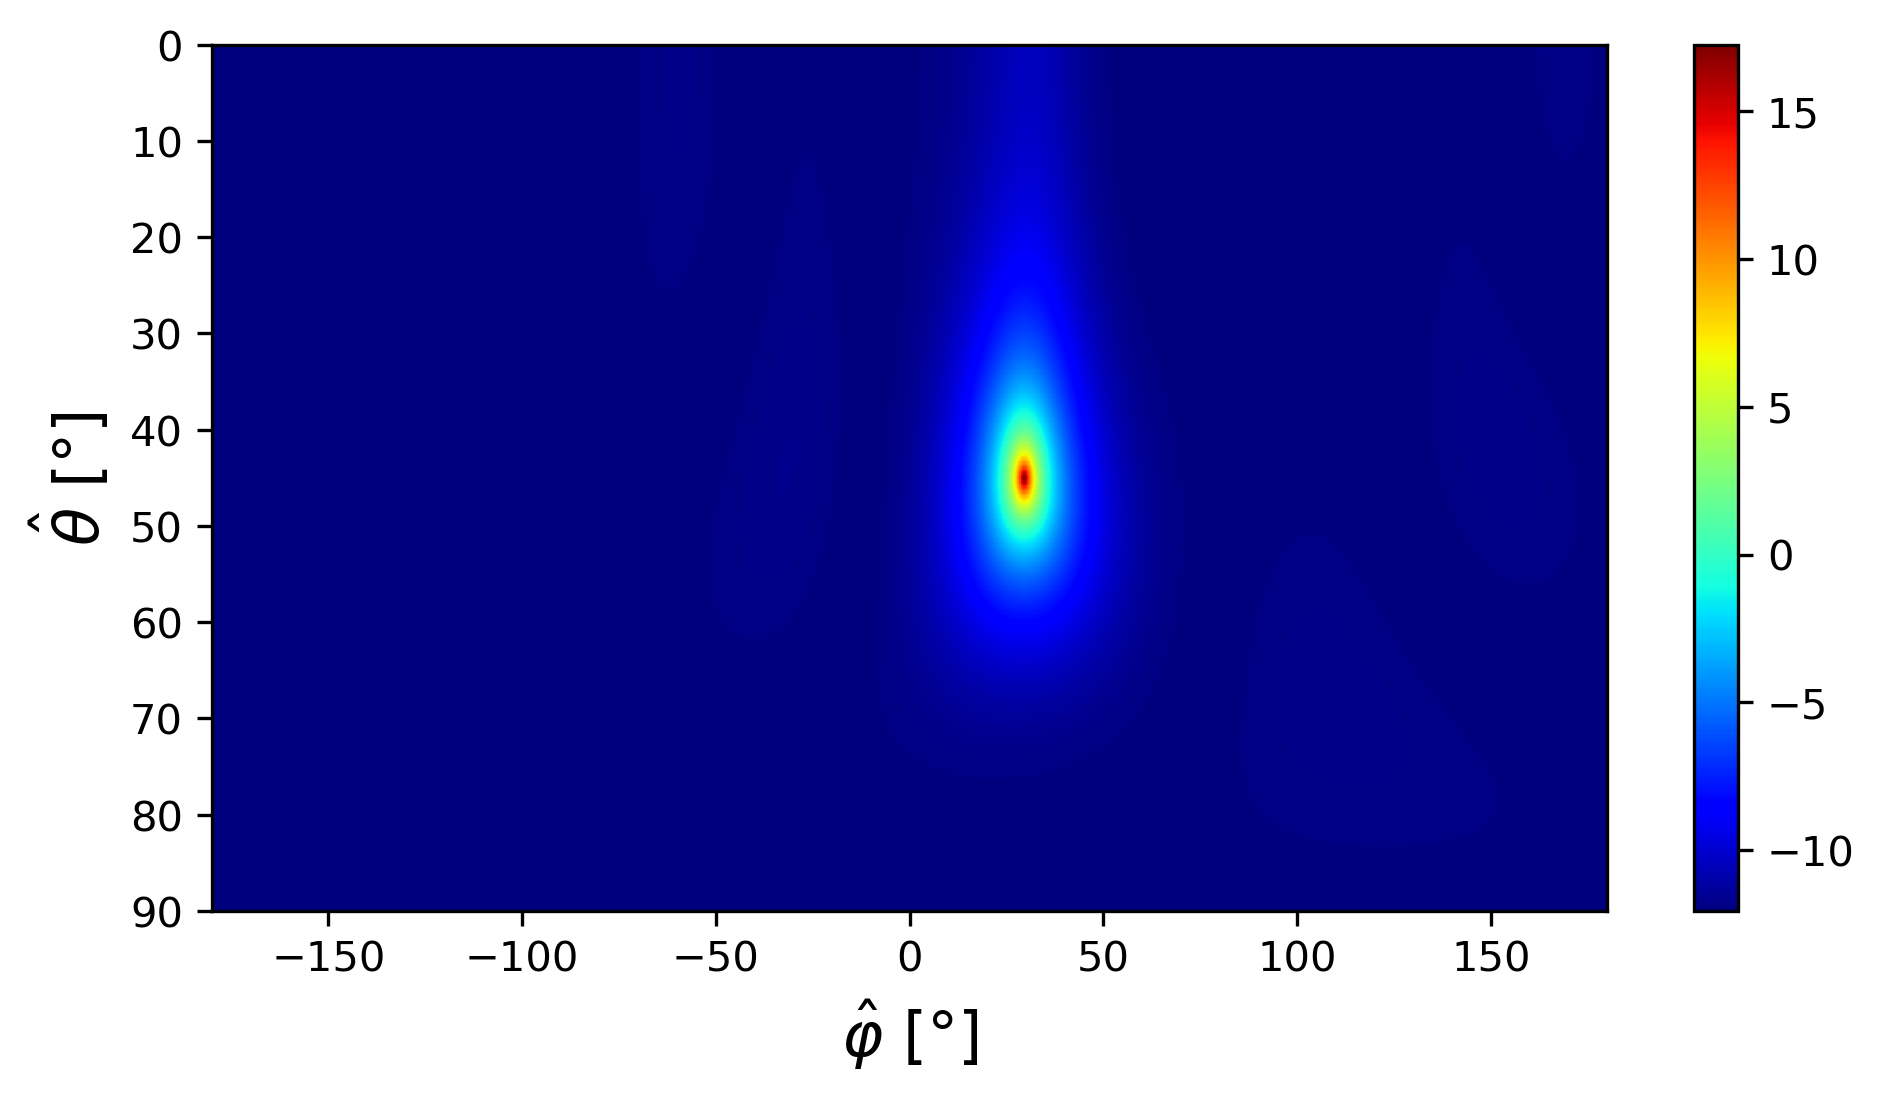
\includegraphics[width=\linewidth]{images/03-DOAEst/p_mu_0.png}
        \caption{SNR = 0 dB}
    \end{subfigure}
    \hfill
    \begin{subfigure}[b]{0.49\textwidth}
        \centering
        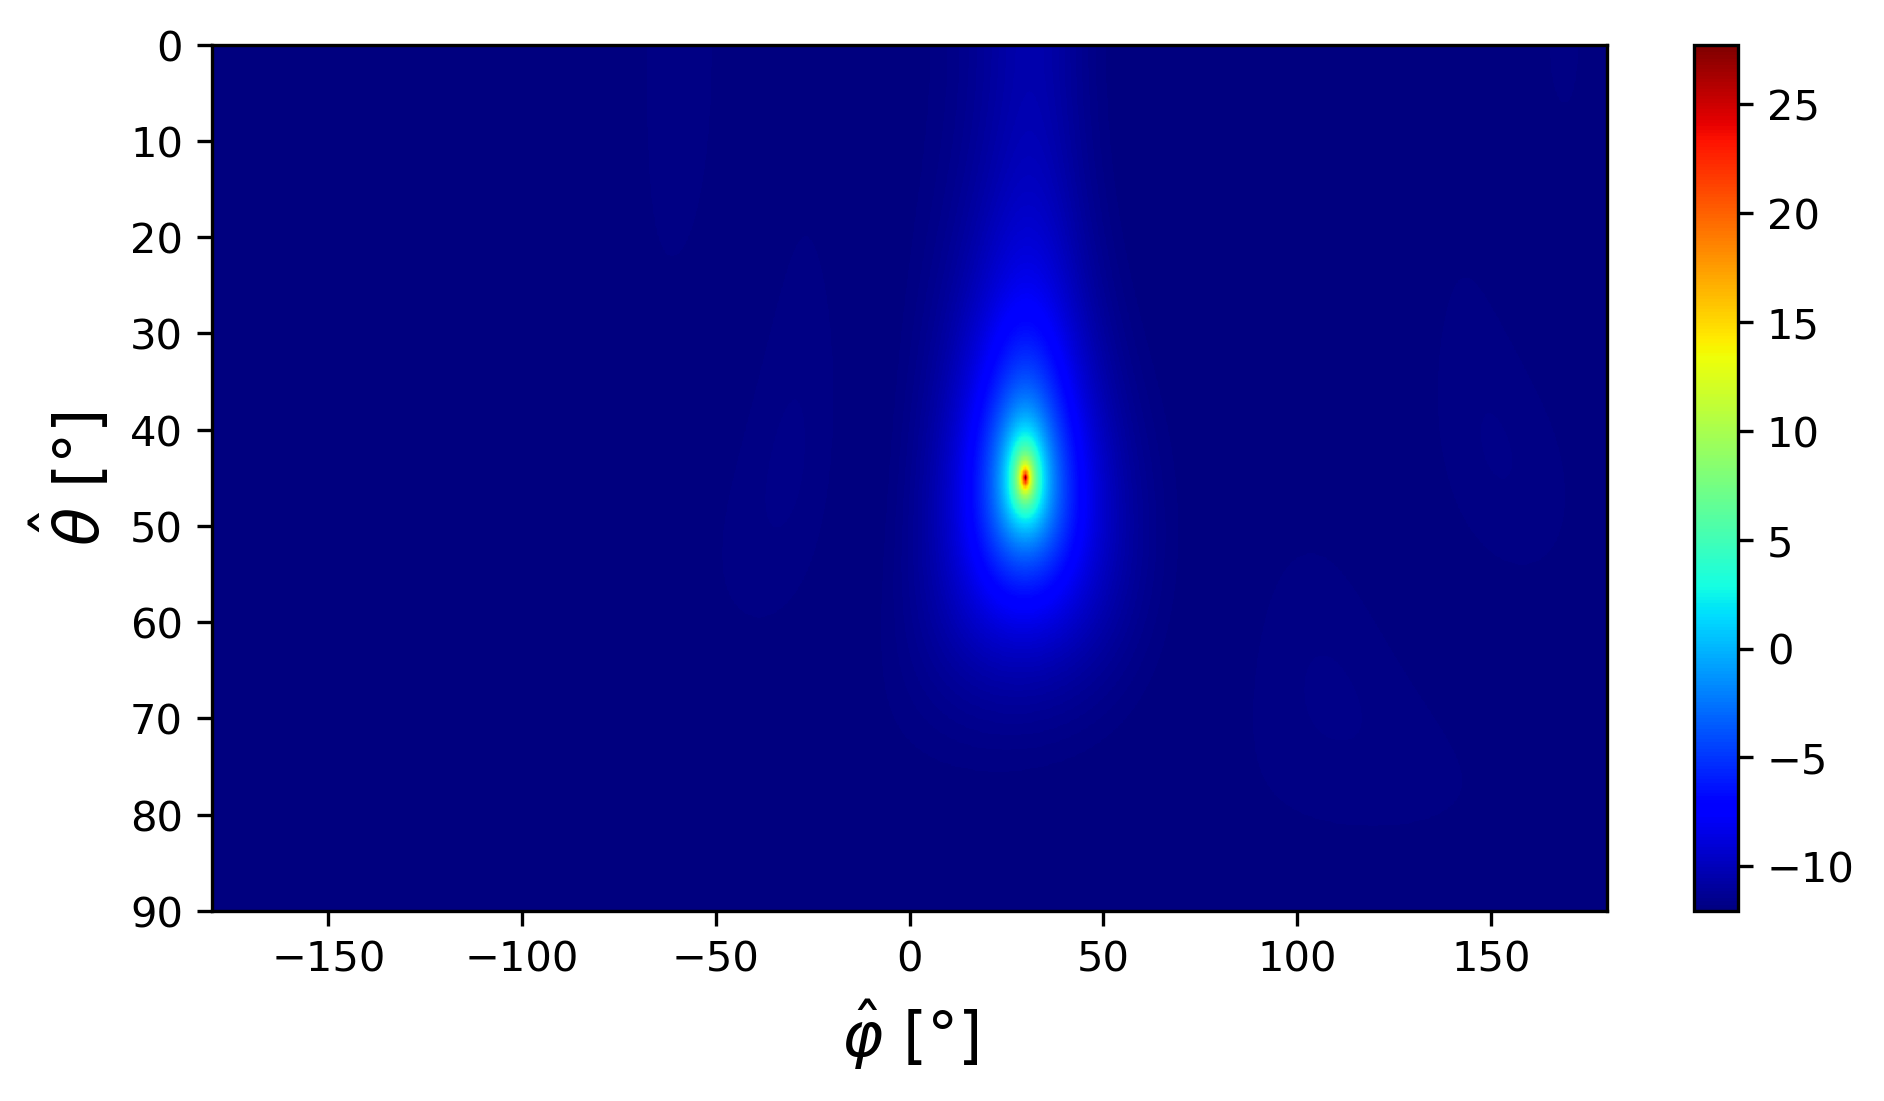
\includegraphics[width=\linewidth]{images/03-DOAEst/p_mu_10.png}
        \caption{SNR = 10 dB}
    \end{subfigure}
    \caption{Gráfica de $\mathbf{P_{MU}}$ en el caso de una señal llegando al arreglo con dirección $(\theta = 45\grad, \varphi=30)$ para distintos valores de SNR. Puede observarse cómo a medida que aumenta la SNR la ``energía'' del pseudoespectro se concentra cada vez más en la dirección de arribo real.}
    \label{fig:doaest_p_mu}
\end{figure}

\subsection{RMSE vs. $\frac{\sigma_d}{d}$}

En este apartado se evalúan ambos algoritmos en función de errores aleatorios en la separación de elementos. Para hacer esto se suman en cada elemento fases aleatorias en ambas dimensiones del arreglo, de manera tal que se simulen errores gaussianos en la ubicación de elementos, ubicando el centro de la gaussiana en el centro de cada uno y tomando como desvío estándar $\sigma_d$ de la distribución distintas fracciones de la distancia entre elementos $d$.
Los parámetros utilizados en esta simulación son:
\begin{itemize}
    \item SNR = 10 dB
    \item $M_x = 4$
    \item $M_y = 4$
    \item $N = 1500$ vectores de muestras
    \item $\mathfrak{R}_{\textrm{MUSIC}}=0,5\grad$
\end{itemize}

Los resultados que se muestran en la Figura \ref{fig:doaest_error_vs_d_error} se obtuvieron promediando 10 realizaciones por cada valor de $\frac{\sigma_d}{d}$. Nuevamente, ambos algoritmos evolucionan de manera similar, manteniendo errores en el orden del grado para desviaciones menores al 5\% en la separación entre elementos.
\begin{figure}[ht!]
    \centering
    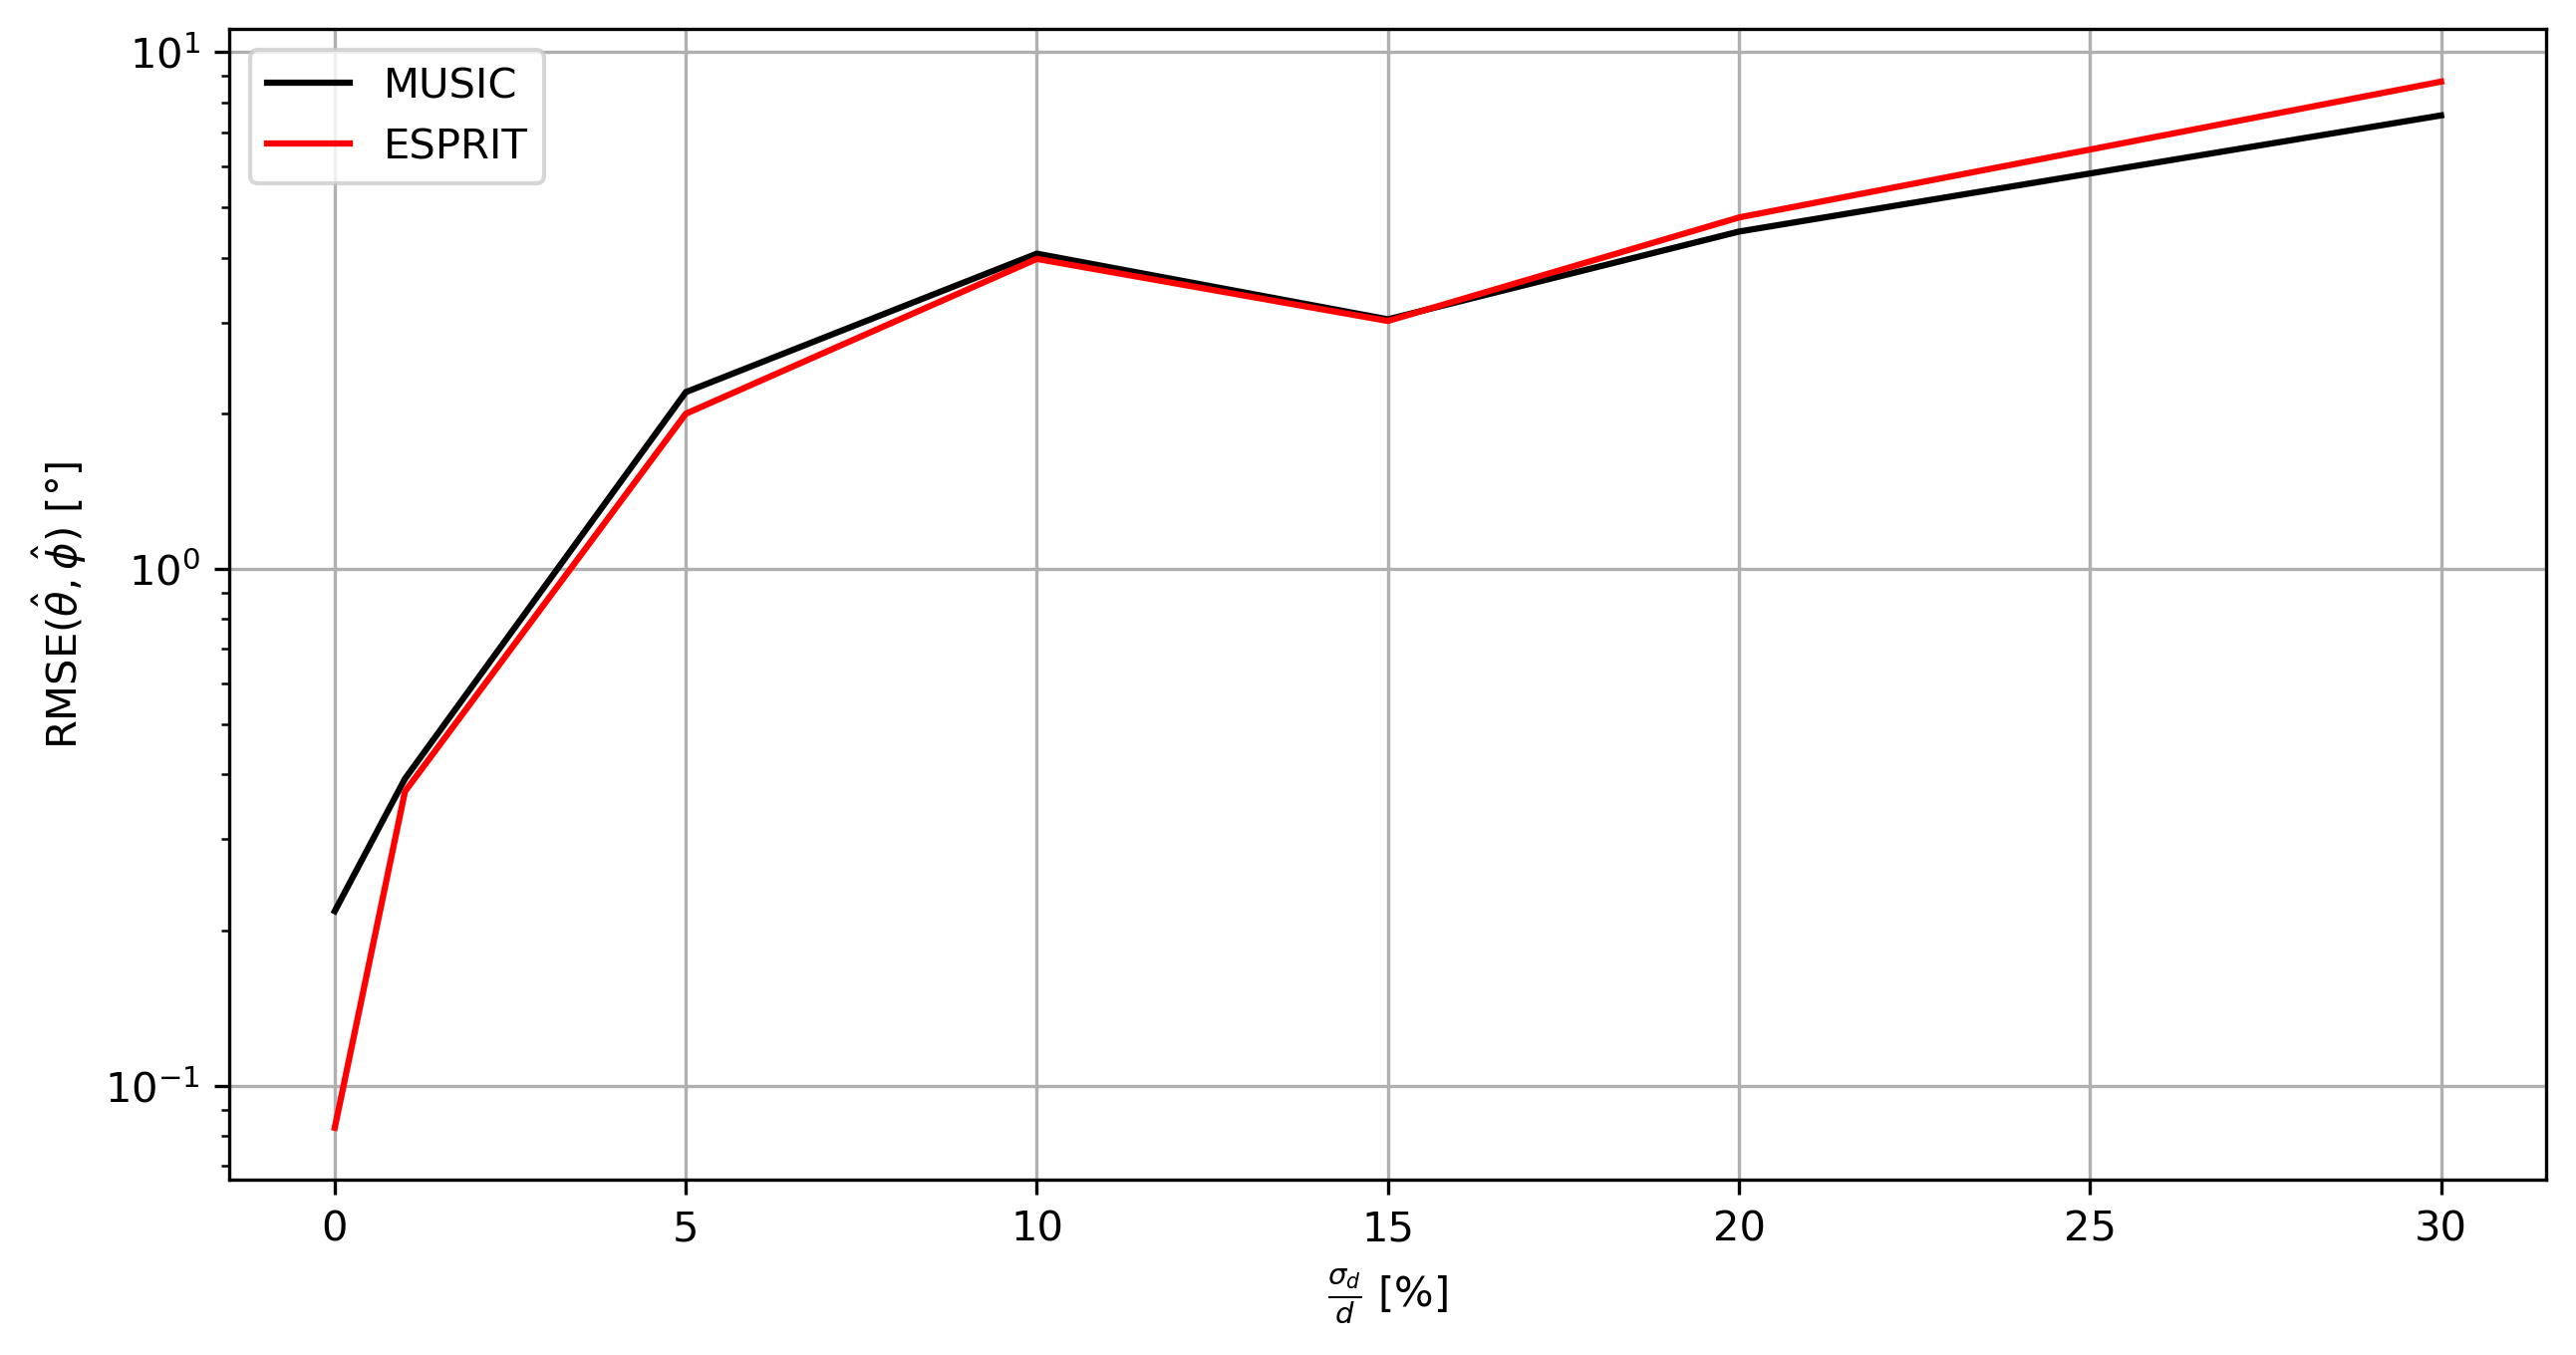
\includegraphics[width=0.9\linewidth]{images/03-DOAEst/error_vs_d_error.png}
    \caption{Gráfico de comparación del RMSE en función de los errores en la separación de elementos para los algoritmos MUSIC y ESPRIT.}
    \label{fig:doaest_error_vs_d_error}
\end{figure}

\subsection{RMSE vs. N° de muestras} %esto quizás habría que meterlo en random sampling

En esta comparación se analiza la variación del RMSE en función de las muestras utilizadas para realizar la estimación con ambos algoritmos. Para esto se repitieron 10 realizaciones por cada valor de $N$, promediándolas. Los parámetros de esta simulación son:
\begin{itemize}
    \item SNR = 10 dB
    \item $M_x = 4$
    \item $M_y = 4$
    \item $\frac{\sigma_d}{d}=0$
    \item $\mathfrak{R}_{\textrm{MUSIC}}=0,5\grad$
\end{itemize}

Los resultados obtenidos se muestran en la Figura \ref{fig:doaest_error_vs_n}. Como puede verse, ambos algoritmos mejoran su desempeño cuantas más muestras reciben debido a la mejor estimación que se logra de los subespacios de señal y de ruido, siguiendo una curva similar en ambos casos. Para el caso de gran cantidad de muestras, MUSIC muestra una asíntota horizontal, producto de su limitada resolución. Sin embargo, para esta SNR elegida, se alcanzan errores menores a la décima del grado utilizando una cantidad de muestras del orden de $10^3$, lo cual computacionalmente no conlleva grandes costos como se mostrará posteriormente.
\begin{figure}[ht!]
    \centering
    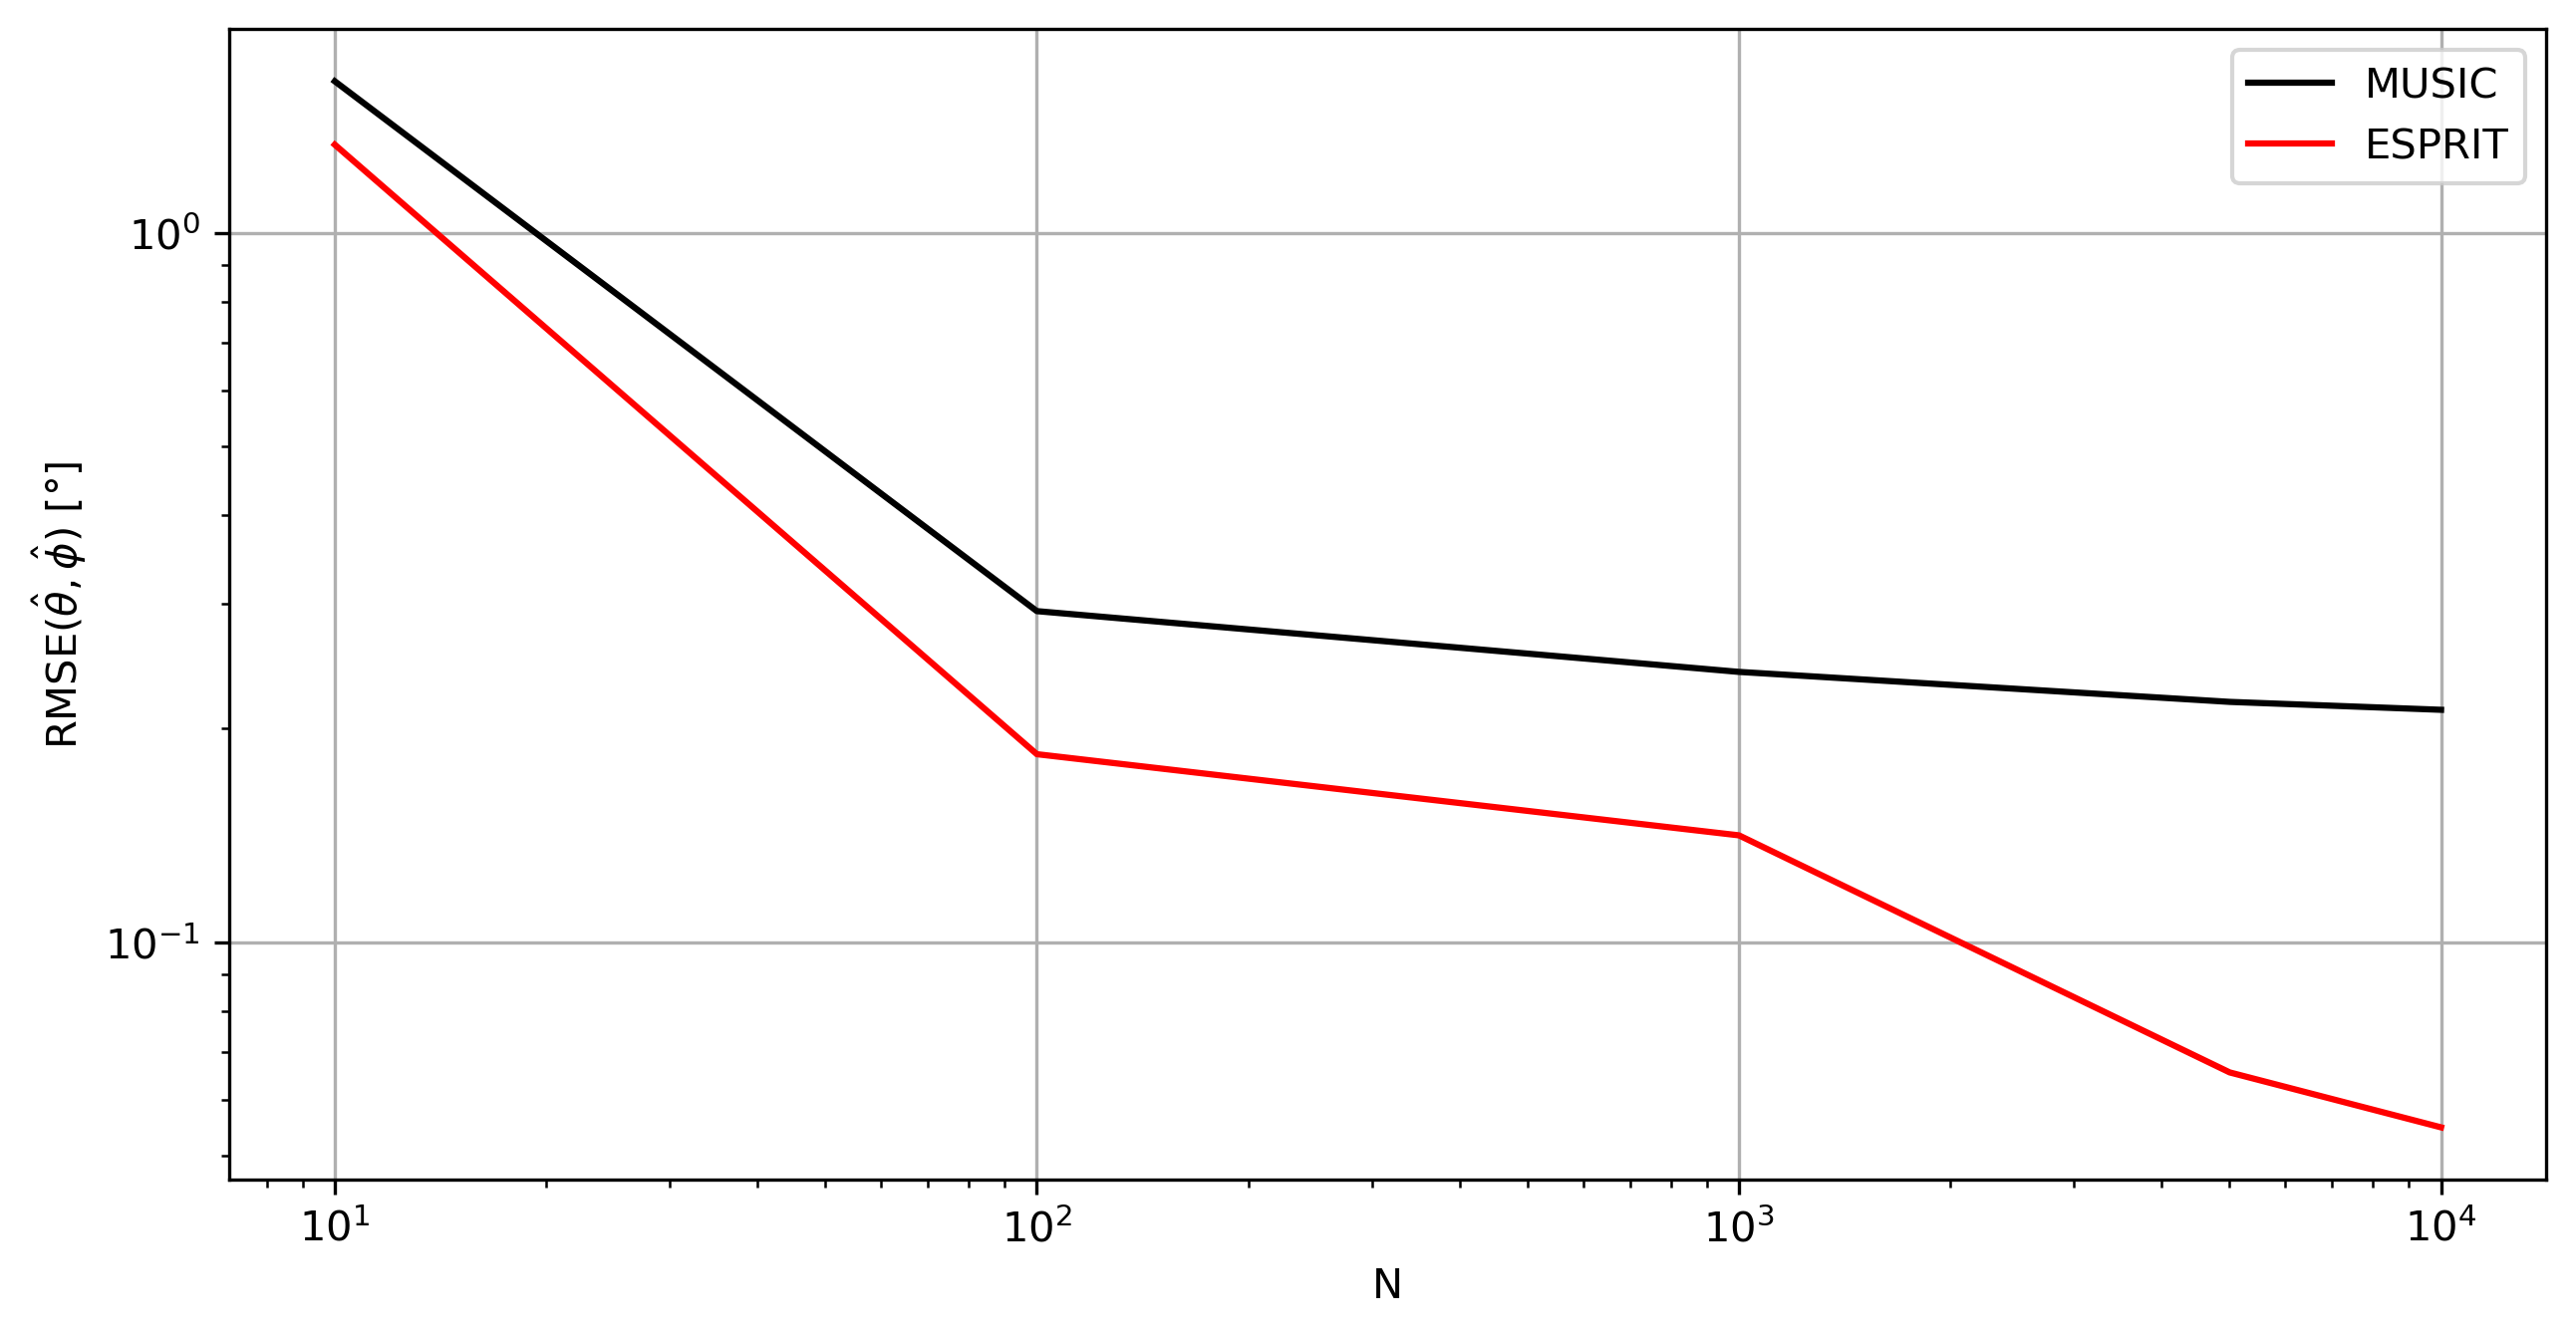
\includegraphics[width=0.9\linewidth]{images/03-DOAEst/error_vs_n.png}
    \caption{Gráfica de comparación del RMSE en función de la cantidad de vectores de muestras para los algoritmos MUSIC y ESPRIT.}
    \label{fig:doaest_error_vs_n}
\end{figure}

%error vs carrierest?
%un error en el valor de la portadora implica un error en el vector de propagación k utilizado para realizar la estimación

\subsection{Tiempo vs. $M$}
En esta sección se comparan los tiempos de ejecución de ambos algoritmos en función de la cantidad de elementos del arreglo. Además, en el caso de MUSIC también se analiza cuánto varían las curvas de tiempo para distintos valores de resoluciones alcanzadas. Para este análisis no se considera el tiempo que se tarda en realizar la SVD debido a que es una tarea común a ambos algoritmos, en cambio este análisis se realiza en la siguiente sección. Por ende, en el caso de MUSIC sólo es evaluado el tiempo que lleva realizar los pasos 5 y 6 del algoritmo desarrollado en la Sección \ref{subc:doaest_music_alg} y en el caso de ESPRIT solo se evalúan los pasos 6 a 11 descriptos en la Sección \ref{subc:doaest_esprit_alg}. Los resultados se muestran en la Figura \ref{fig:tiempo_vs_m}. Los parámetros definidos para esta simulación son:
\begin{itemize}
    \item SNR = 10 dB
    \item $\frac{\sigma_d}{d}=0$
    \item $N=1500$ vectores de muestras
\end{itemize}
\begin{figure}[ht!]
    \centering
    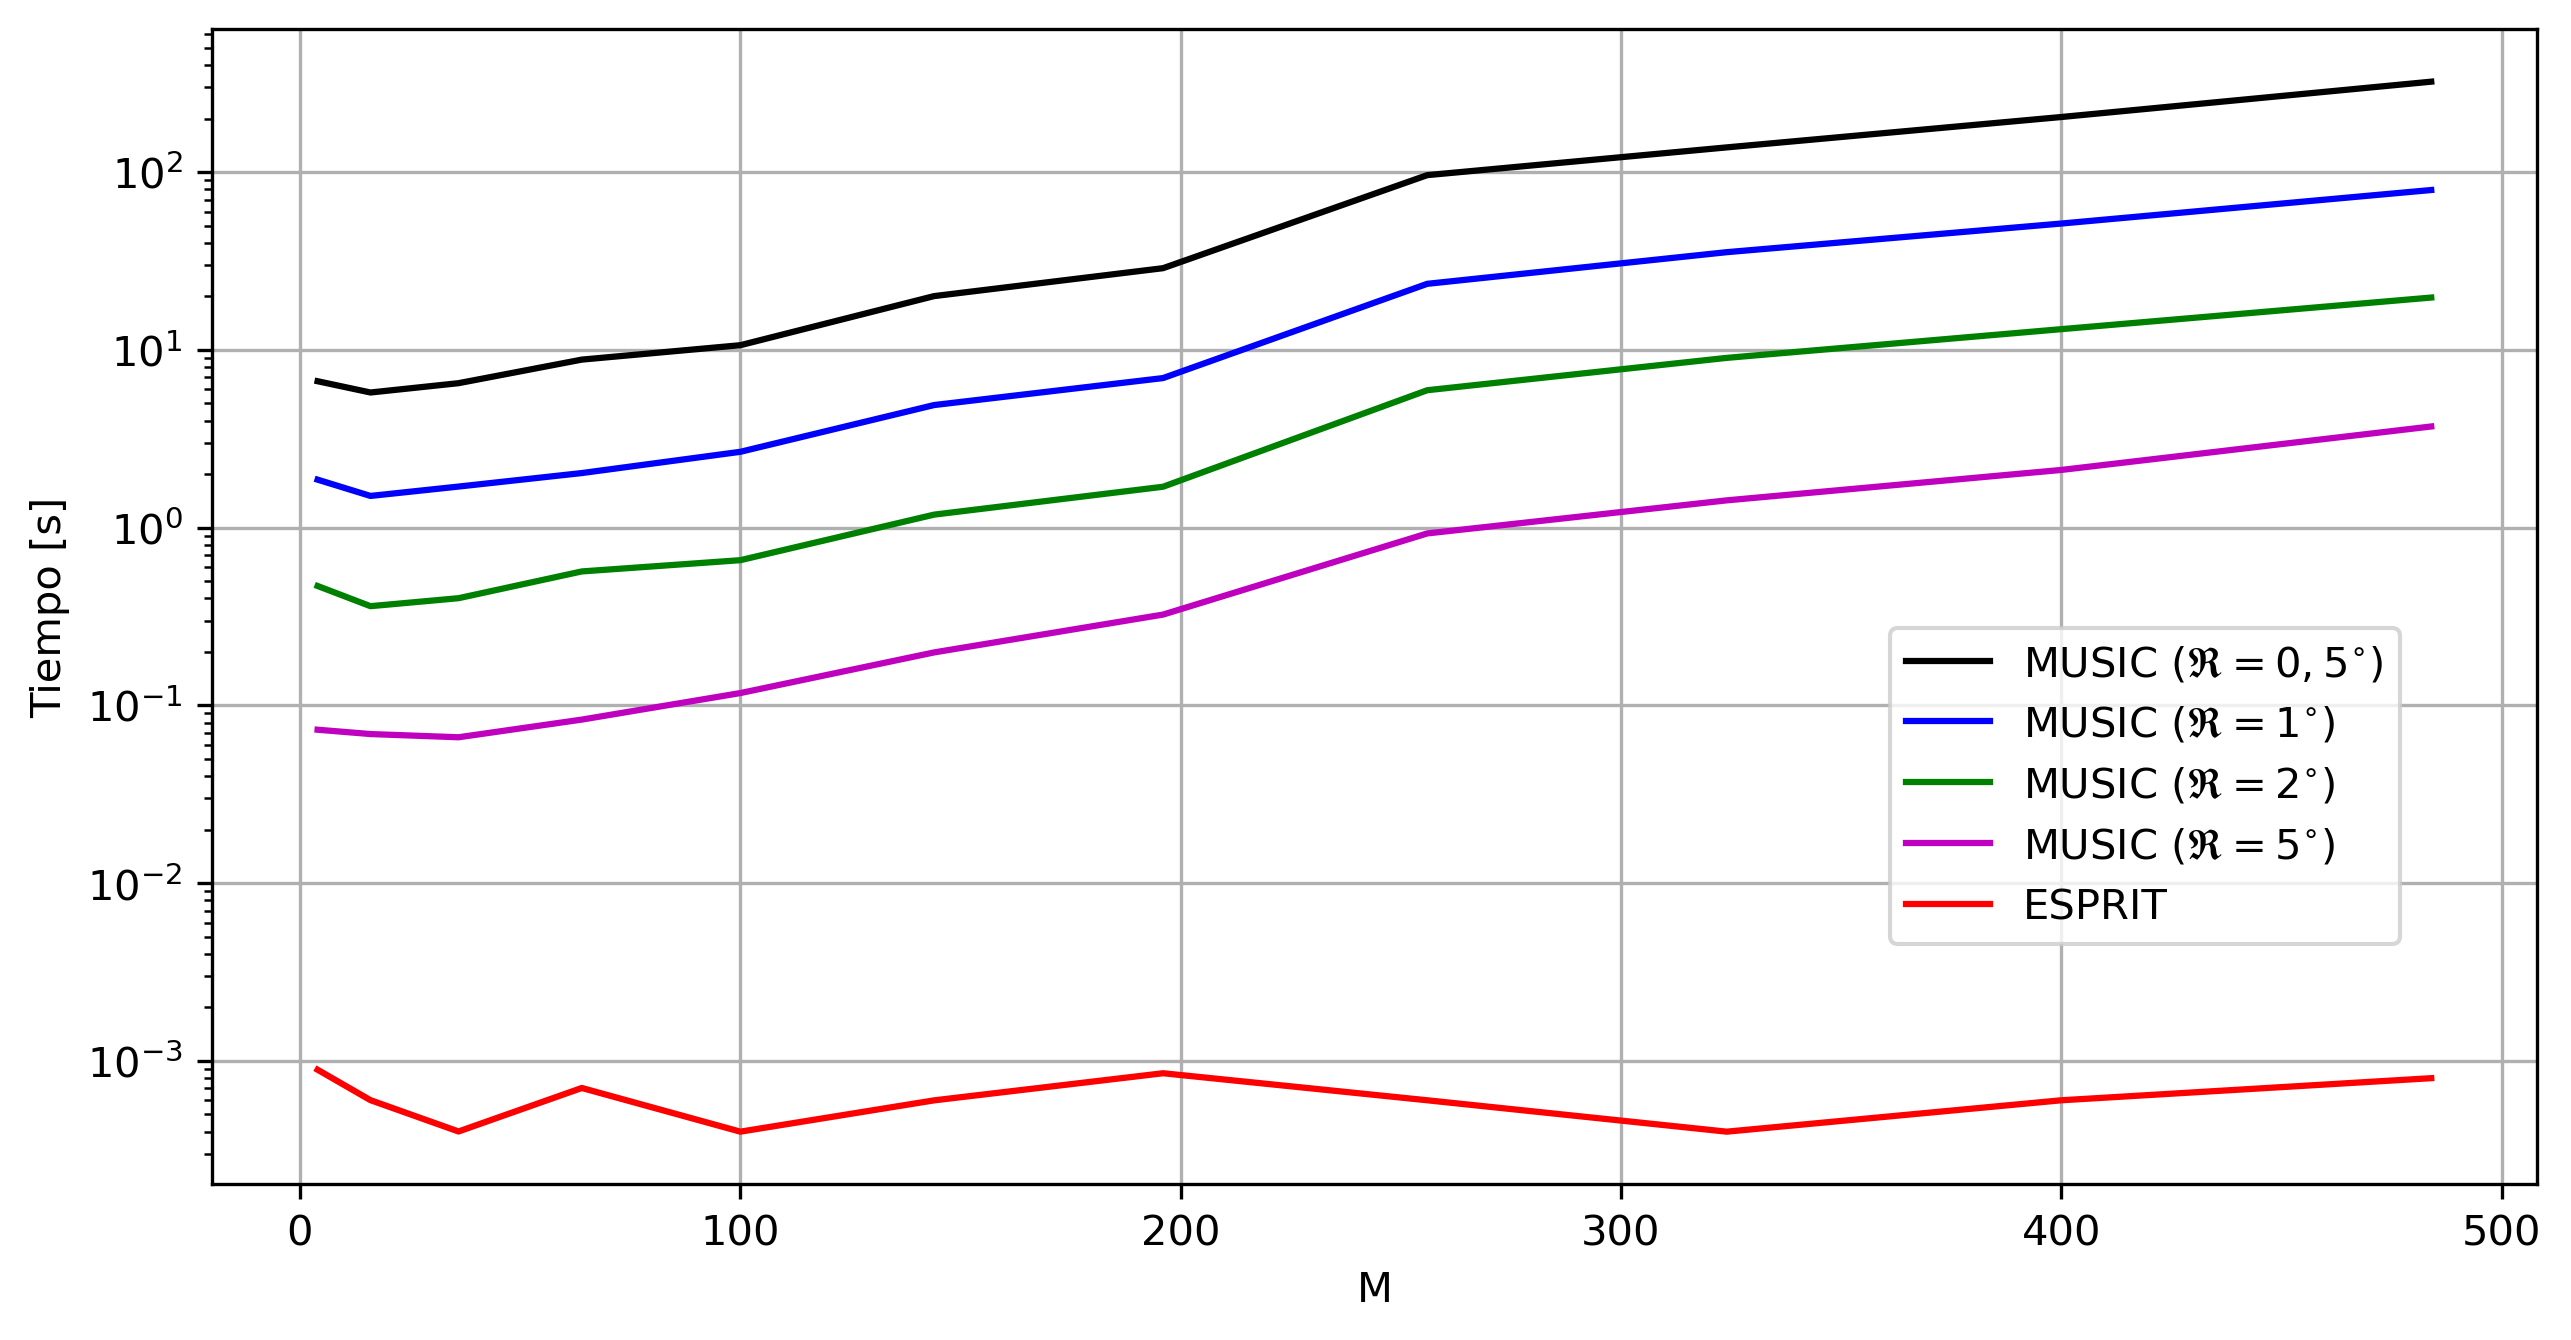
\includegraphics[width=0.9\linewidth]{images/03-DOAEst/time_vs_m.png}
    \caption{Gráfica de comparación del tiempo de ejecución de los algoritmos MUSIC y ESPRIT en función de la cantidad de elementos del ARU.}
    \label{fig:tiempo_vs_m}
\end{figure}

Como puede verse, para todos los valores de cantidad de elementos analizados, el algoritmo MUSIC resultó ser mucho menos eficiente que ESPRIT, obteniendo tiempos de al menos dos órdenes de magnitud mayor para $M<100$ y tres órdenes mayor para $M>300$ para una resolución en la estimación de $\mathfrak{R_{\textrm{MUSIC}}}=5\grad$. Además, si se analiza la curva de tiempos de MUSIC para una resolución de $\mathfrak{R_{\textrm{MUSIC}}}=0,5\grad$, la cual brinda un nivel de error semejante a ESPRIT como se mostró en la Sección \ref{subc:doaest_error_vs_snr}, el tiempo de ejecución supera al ESPRIT por más de 5 órdenes de magnitud. Esto provoca que esta implementación del MUSIC sea ineficiente para aplicaciones de tiempo real como la que se desea desarrollar en este proyecto. El motivo del incremento del costo computacional del MUSIC con respecto a $M$ se debe al cálculo de la Ecuación \ref{eq:doaest_pmu}, ya que todas las matrices que entran en la multiplicación tienen $M$ filas, y la matriz $\mathbf{\hat{E}_W}$ tiene mayor cantidad de columnas cuanto mayor sea M, lo que provoca que la cantidad de operaciones a realizar crezca rápidamente a medida que aumenta $M$. En cambio el algoritmo ESPRIT reduce la dimensión del problema separando  $\mathbf{\hat{E}_S}$ en  $\mathbf{\hat{E}_X}$ y  $\mathbf{\hat{E}_Y}$ para armar  $\mathbf{\hat{E}_{XY}}$ la cual como máximo puede tener una cantidad de filas de $M-1$. Esta matriz solo es utilizada cuando se le aplica la descomposición en valores singulares, momento en el cual se comienza a operar con matrices de tamaño $D\times D$, siendo $D<M$. La complejidad de ambos algoritmos aumenta con el aumento en la cantidad de señales a estimar.

Si se analizan las variaciones de tiempo entre distintas resoluciones de la solución brindada por MUSIC el motivo del crecimiento del costo a medida que se aumenta la resolución radica en el dominio de búsqueda en el que se debe calcular la Ecuación \ref{eq:doaest_pmu}, ya que una mayor resolución implica mayores puntos del dominio donde se desea saber el valor de $\mathbf{P_{MU}}(\theta,\varphi)$. El dominio de búsqueda puede reducirse a partir de la utilización de información previa sobre las direcciones de arribo estimadas, sin embargo la gran eficiencia de ESPRIT no motivó la realización de ese estudio para este trabajo.

\subsection{Tiempo de ejecución de la SVD}

En esta sección se analiza el costo computacional del algoritmo SVD implementado dentro de la librería \texttt{NumPy} \cite{bib:numpy} en función de la cantidad de elementos del arreglo $M$ y la cantidad de vectores de muestras con el que se alimenta a algoritmo $N$. Debido a que en la simulación en función de $M$ vamos a estar variando la cantidad de filas de la matriz $\mathbf{X}$ definida en la Ecuación \ref{eq:doaest_x} y en la simulación en función de $N$ vamos a estar variando las columnas se decidió que la variable que quede fija en cada una tenga el mismo valor, lo cual se logró fijando la cantidad de elementos del arreglo en 100 para la simulación en función de $N$ y fijando la cantidad de vectores de muestras en 100 para la simulación en función de $M$. Por ende, los parámetros utilizados en estas simulaciones son los siguientes:
\begin{itemize}
    \item SNR = 10 dB
    \item $M_x = 10$ (solo para el análisis en función de $N$)
    \item $M_y = 10$ (solo para el análisis en función de $N$)
    \item $N = 100$ vectores de muestras (solo para el análisis en función de $M$)
    \item $\frac{\sigma_d}{d}=0$
\end{itemize}
obteniendo los resultados que se indican en la Figura \ref{fig:svd_vs_n_m}.
\begin{figure}[ht!]
    \centering
    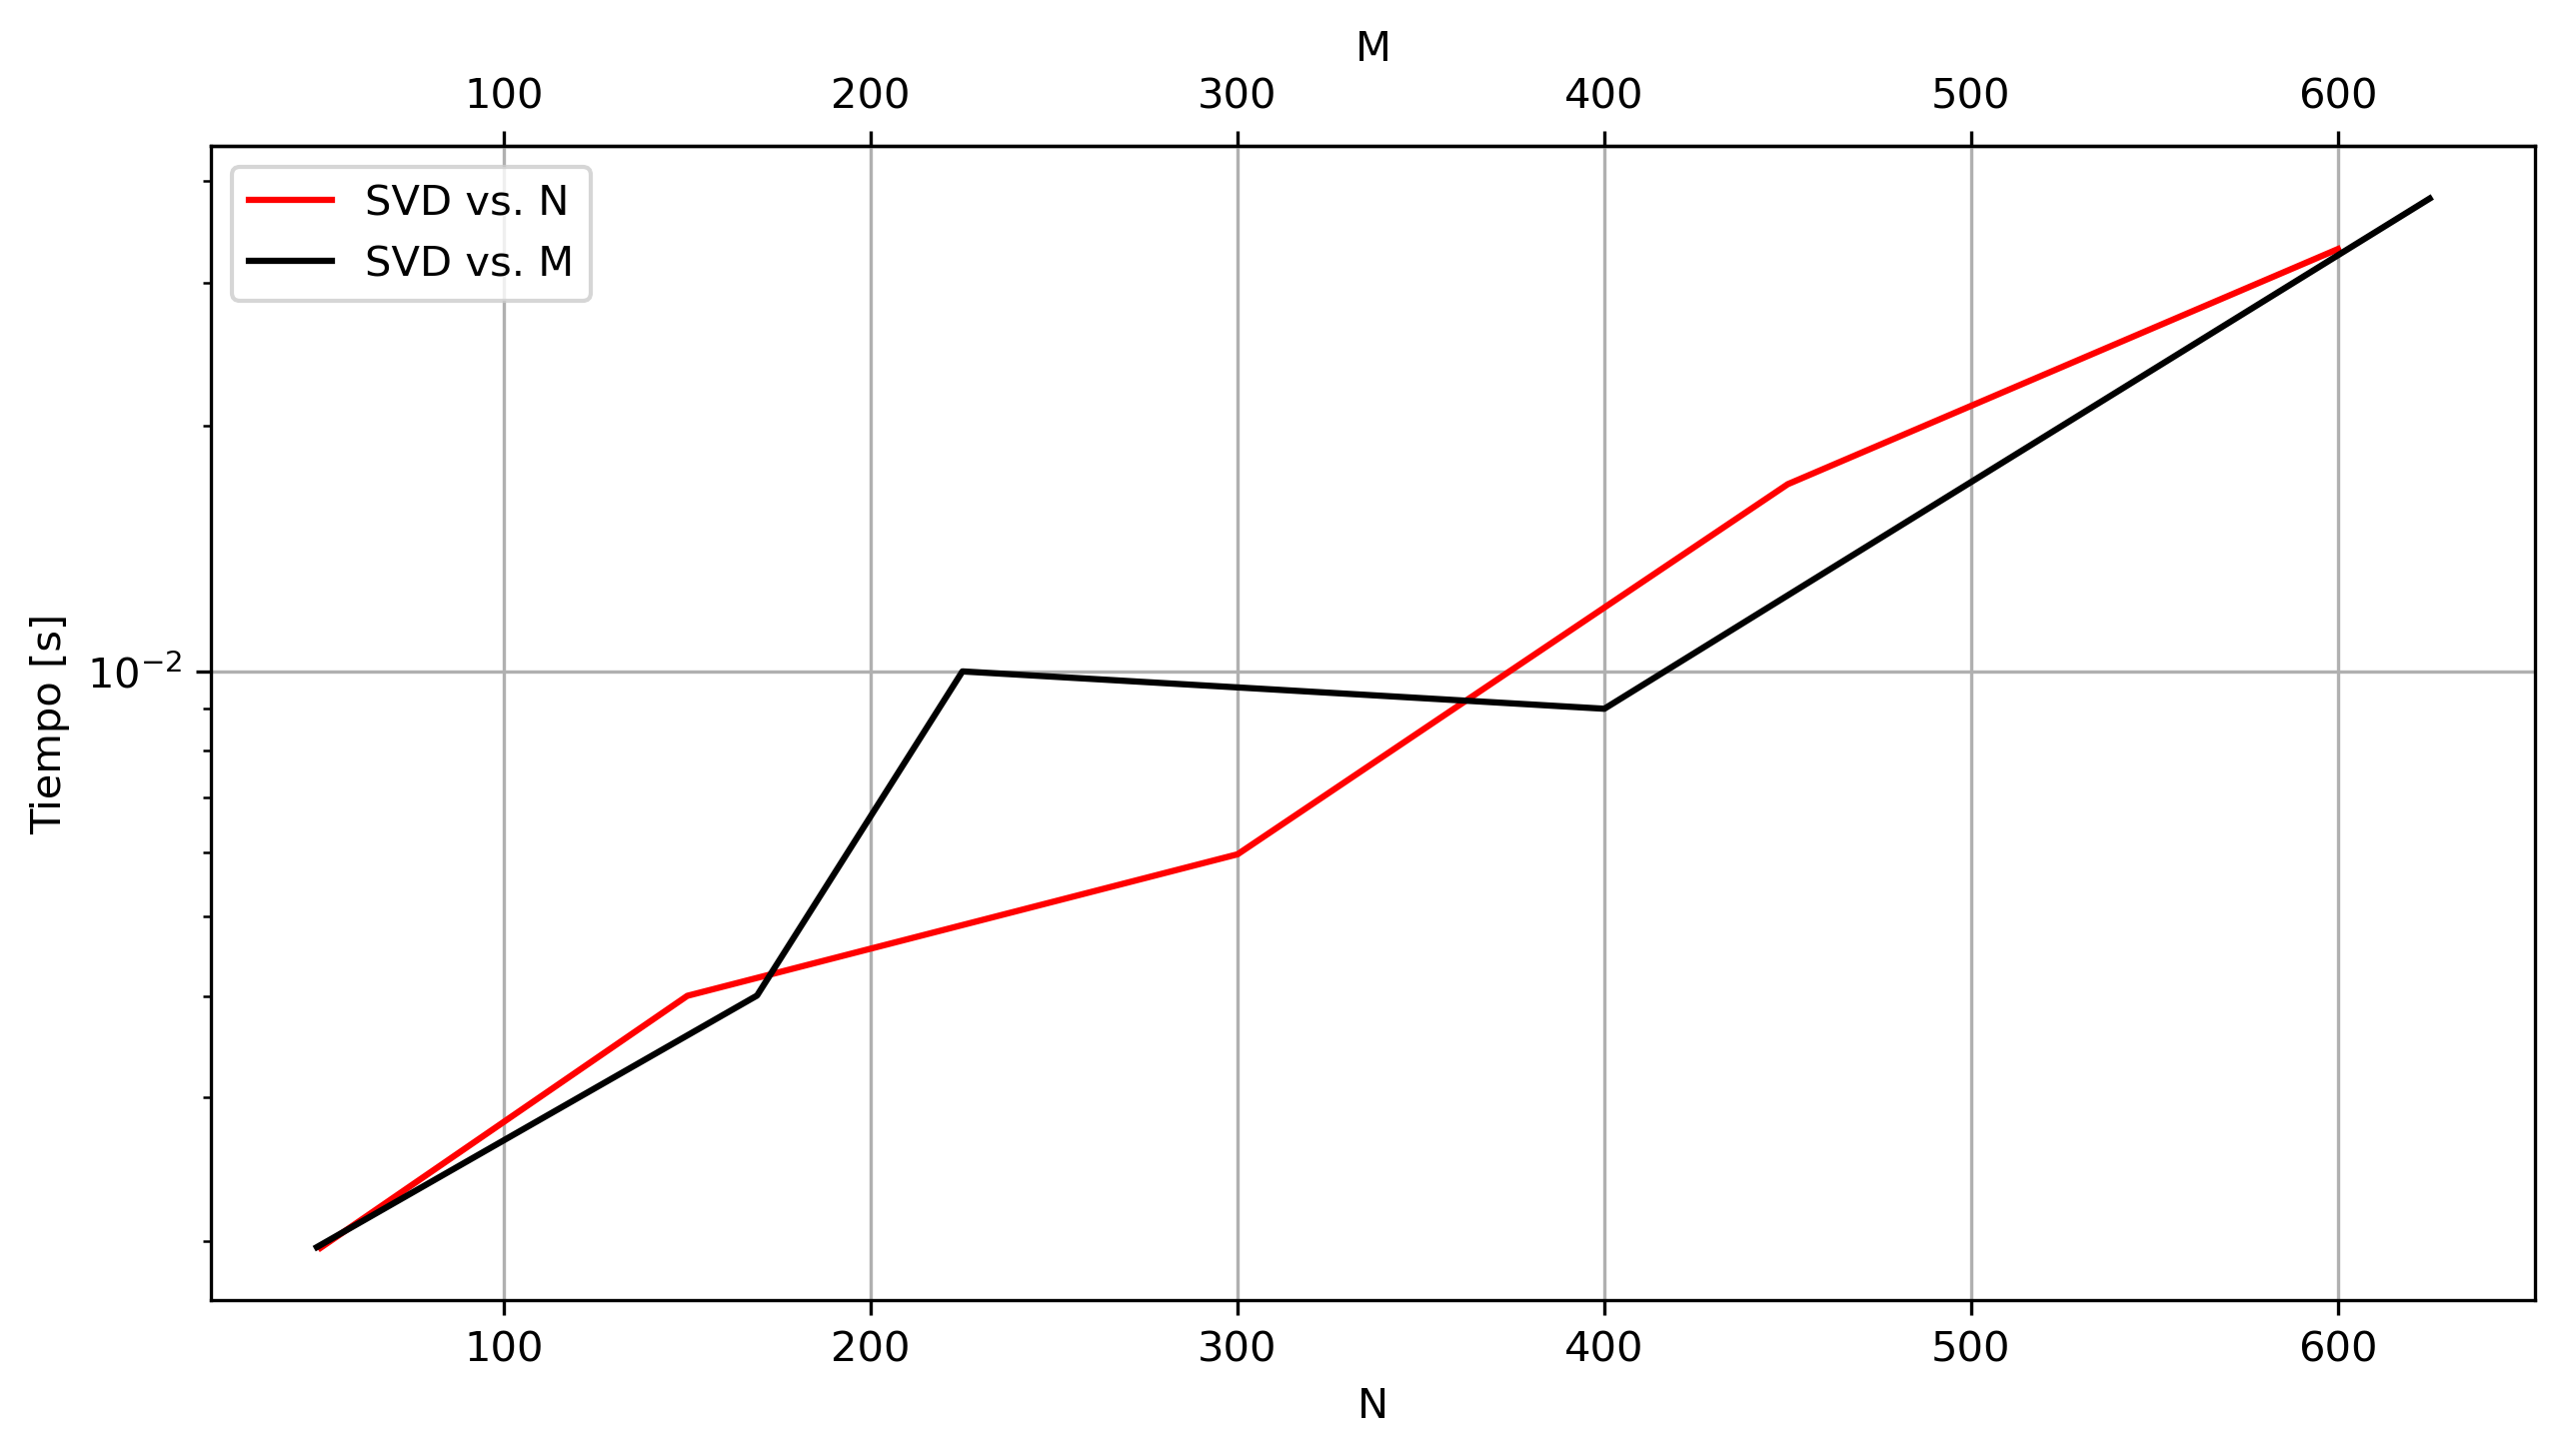
\includegraphics[width=0.9\linewidth]{images/03-DOAEst/svd_vs_n_m.png}
    \caption{Gráfica de tiempo de ejecución del algoritmo SVD en función de la cantidad $M$ de elementos del ARU y la cantidad $N$ de vectores de muestras de la entrada.}
    \label{fig:svd_vs_n_m}
\end{figure}

Como puede observarse, ambas simulaciones evolucionan de manera similar en todos los rangos, lo cual indica que este algoritmo no muestra preferencias con respecto a las dimensiones de la matriz de entrada. Siendo que para la aplicación de este proyecto se espera una cantidad fija de 16 elementos en el arreglo la gráfica que más interesa en este momento es la del tiempo de cómputo de la SVD en función de $N$, ya que indica a partir de qué cantidad de muestras este algoritmo complica la conformación de un sistema que opere en tiempo real. Es por esto que en la Figura \ref{fig:svd_vs_n_16} se muestra una nueva simulación del tiempo de cómputo de la SVD en función de $N$ pero fijando $M$ en 16 elementos.
\begin{figure}[ht!]
    \centering
    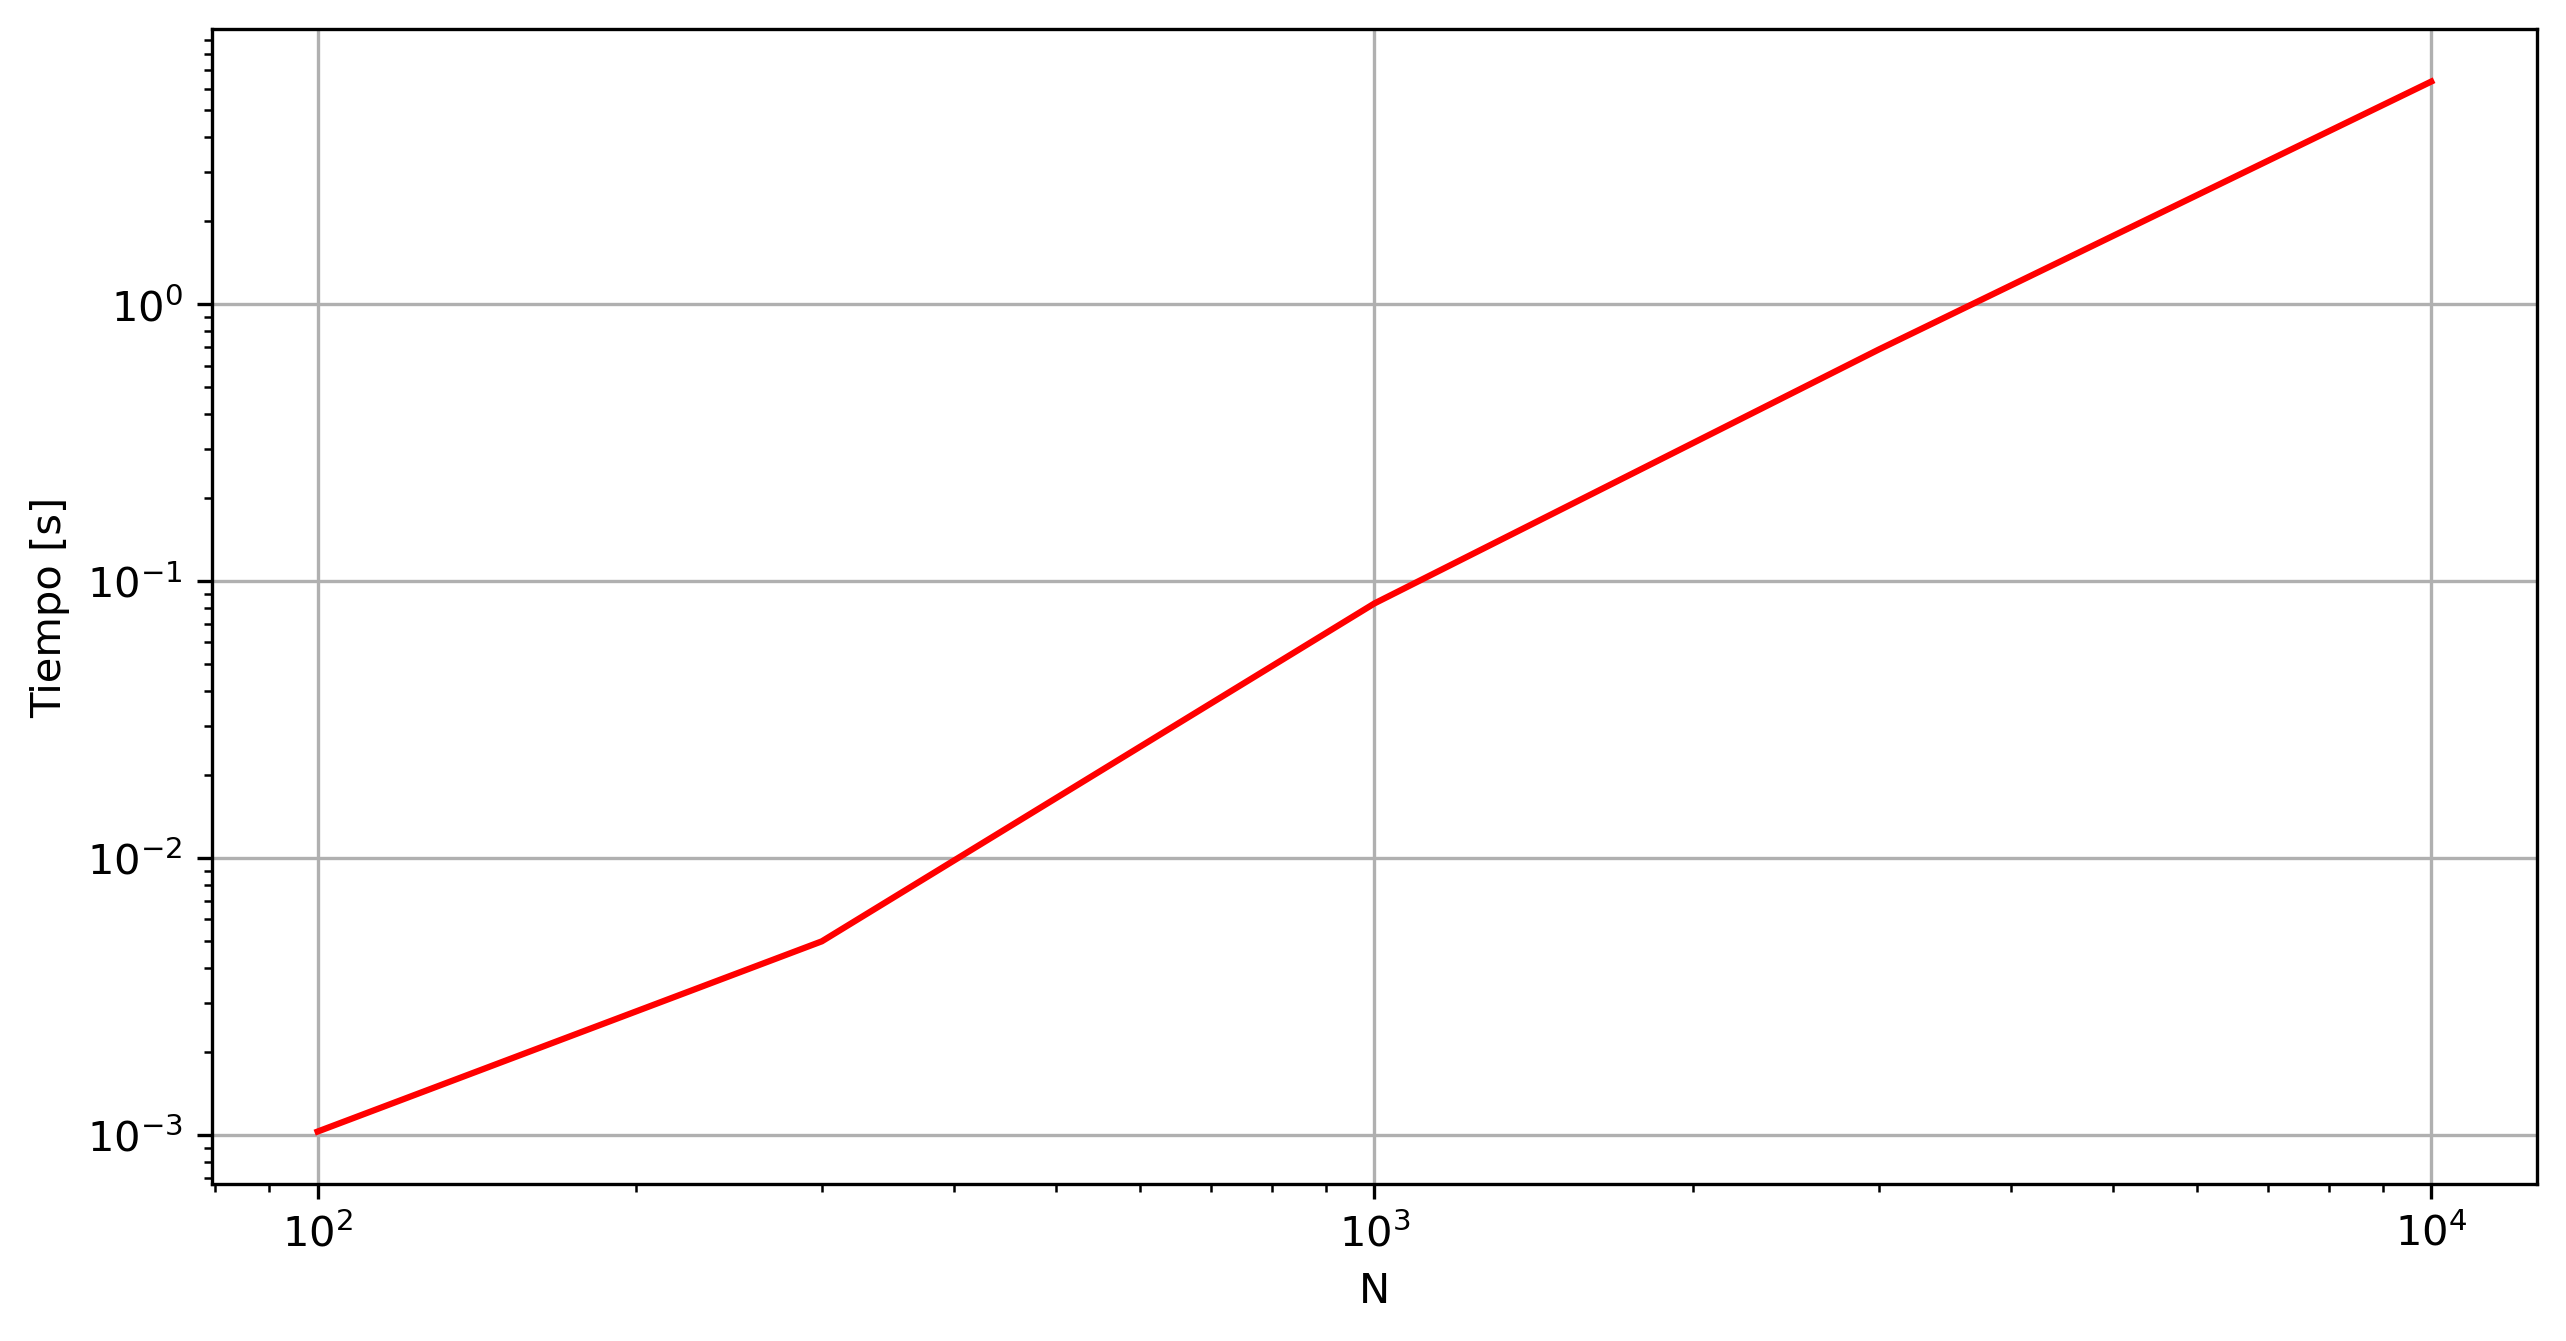
\includegraphics[width=0.9\linewidth]{images/03-DOAEst/svd_vs_n_16.png}
    \caption{Gráfica de tiempo de ejecución del algoritmo SVD en función de la cantidad $N$ de vectores de muestras de la entrada con $M=16$.}
    \label{fig:svd_vs_n_16}
\end{figure}

Aquí puede verse que, para una cantidad de 16 elementos en el arreglo, la SVD puede realizarse en tiempos menores a la décima de segundo para una cantidad de vectores de muestras del orden de $N=10^3$, y tiempos menores a la centésima de segundo con una cantidad de vectores del orden de $N=500$. También puede verse que la complejidad de esta operación es $O(MN^2)$, como sugiere la teoría \cite{bib:esprit_roy}. A partir de esta gráfica y la gráfica de la Figura \ref{fig:doaest_error_vs_n} puede escogerse una tolerancia al error y un tiempo de ejecución para un cierto valor de SNR y así luego escoger la cantidad de muestras con las cuales se va a trabajar en la implementación real.

% pseudoespectro music vs snr

\chapter{Muestreo aleatorio}\label{ch:randomsampling}
%\chapterquote{Hablaban siempre de dinero y planeaban asaltar un banco}{Domingo Cavallo, 2001}

\section{Conceptos generales}\label{subc:intro_congen}



\chapter{Machine Learning aplicado a la clasificación de autovalores}\label{ch:machinelearning}
%\chapterquote{Hablaban siempre de dinero y planeaban asaltar un banco}{Domingo Cavallo, 2001}

\section{Conceptos generales}\label{subc:intro_congen}



\chapter{Diseño del sistema}\label{ch:sistema}
\chapterquote{Los ingenieros hacemos realidad las utopías de los físicos.}{Julio Benitez}

\section{Introducción}\label{subc:sistema_intro}
A esta altura ya se cuenta con los conocimientos teóricos sobre todas las tareas que debe cumplir el sistema conformador de haz. En particular este debe ser capaz de:
\begin{itemize}
    \item Muestrear aleatoriamente con el algoritmo detallado en el Capítulo \ref{ch:randomsampling} los vectores de muestras provenientes del sistema de adquisición encargado de muestrear al ARU.
    \item Estimar la cantidad de señales recibidas utilizando el algoritmo SVM analizado en la Sección \ref{subc:ml_svm}.
    \item Estimar la dirección de arribo de cada una de las señales recibidas utilizando el algoritmo ESPRIT que se detalló en la Sección \ref{subc:doaest_ESPRIT}.
    \item Con la información obtenida de la estimación de cantidad de señales y estimación de direcciones de arribo realizar la conformación de haz de cada una de las señales detectadas.
\end{itemize}

Este sistema correrá en una placa de desarrollo CIAA-ACC, la cual cuenta con un SoC \footnote{\emph{System on a chip,} circuito integrado que concentra una gran variedad de recursos en un solo chip.} Xilinx Zynq-7030 \cite{bib:zynq}, el cual integra, por un lado, \emph{lógica programable} (PL) bajo la forma de un dispositivo FPGA de la familia Kintex-7, y por otro, un \emph{sistema de procesamiento} (PS) con dos microprocesadores ARM Cortex-A9. Esto brinda la posibilidad de implementar bloques en distintas arquitecturas pudiendo así explotar las virtudes de cada una, como lo es la posibilidad de optimizar cálculos paralelizables en la PL o la posibilidad de utilizar librerías o lenguajes de alto nivel en el PS. Teniendo esto en cuenta se realizará un diagrama de bloques del sistema en su totalidad para luego hacer hincapié en cada uno de los subsistemas, analizando qué ventajas ofrece su implementación en distintas arquitecturas. Este sistema, además, compartirá los recursos de la PL y del PS con un sistema de adquisición encargado de obtener las muestras digitales simultáneamente de los 16 elementos del ARU. Esta información será de importancia para definir la ubicación y las interfaces de los subsistemas desarrollados en este proyecto y el sistema de adquisición.

A lo largo de este capítulo se utilizará el siguiente esquema de colores para identificar los tipos de datos de las interfaces de los distintos sistemas:
\begin{itemize}
    \item \fcolorbox{blue}{blue}{\rule{0pt}{6pt}\rule{6pt}{0pt}}\quad Datos complejos.
    \item \fcolorbox{Blue}{Blue}{\rule{0pt}{6pt}\rule{6pt}{0pt}}\quad Vectores o matrices de datos complejos.
    \item \fcolorbox{Orange}{Orange}{\rule{0pt}{6pt}\rule{6pt}{0pt}}\quad Vectores o matrices de datos reales.
    \item \fcolorbox{magenta}{magenta}{\rule{0pt}{6pt}\rule{6pt}{0pt}}\quad Datos enteros.
\end{itemize}

\section{Diagrama de bloques del sistema}\label{subc:sistema_bloques}

Conociendo las tareas que debe cumplir el sistema a diseñar se propone el desglose en subsistemas que se muestra en el diagrama de bloques de la Figura \ref{fig:sistema_bd}. El sistema conformador de haz recibe desde un sistema de adquisición matrices de muestras complejas $\mathbf{X}$ de tamaño $M\times N$, como se definió en la Ecuación \ref{eq:doaest_x}, donde $M$ es la cantidad de elementos en el ARU y $N$ es la cantidad de veces que se muestreó al arreglo de antenas en un determinado tiempo. Este sistema está conformado por tres subsistemas que se encargan de realizar el muestreo aleatorio de la matriz de entrada, la estimación de DOA y cantidad de señales recibidas y finalmente la conformación de las señales detectadas, las cuales son entregadas como muestras complejas en las $D$ salidas del sistema, siendo $D$ la cantidad de señales detectadas.

\begin{figure}[ht!]
    \centering
    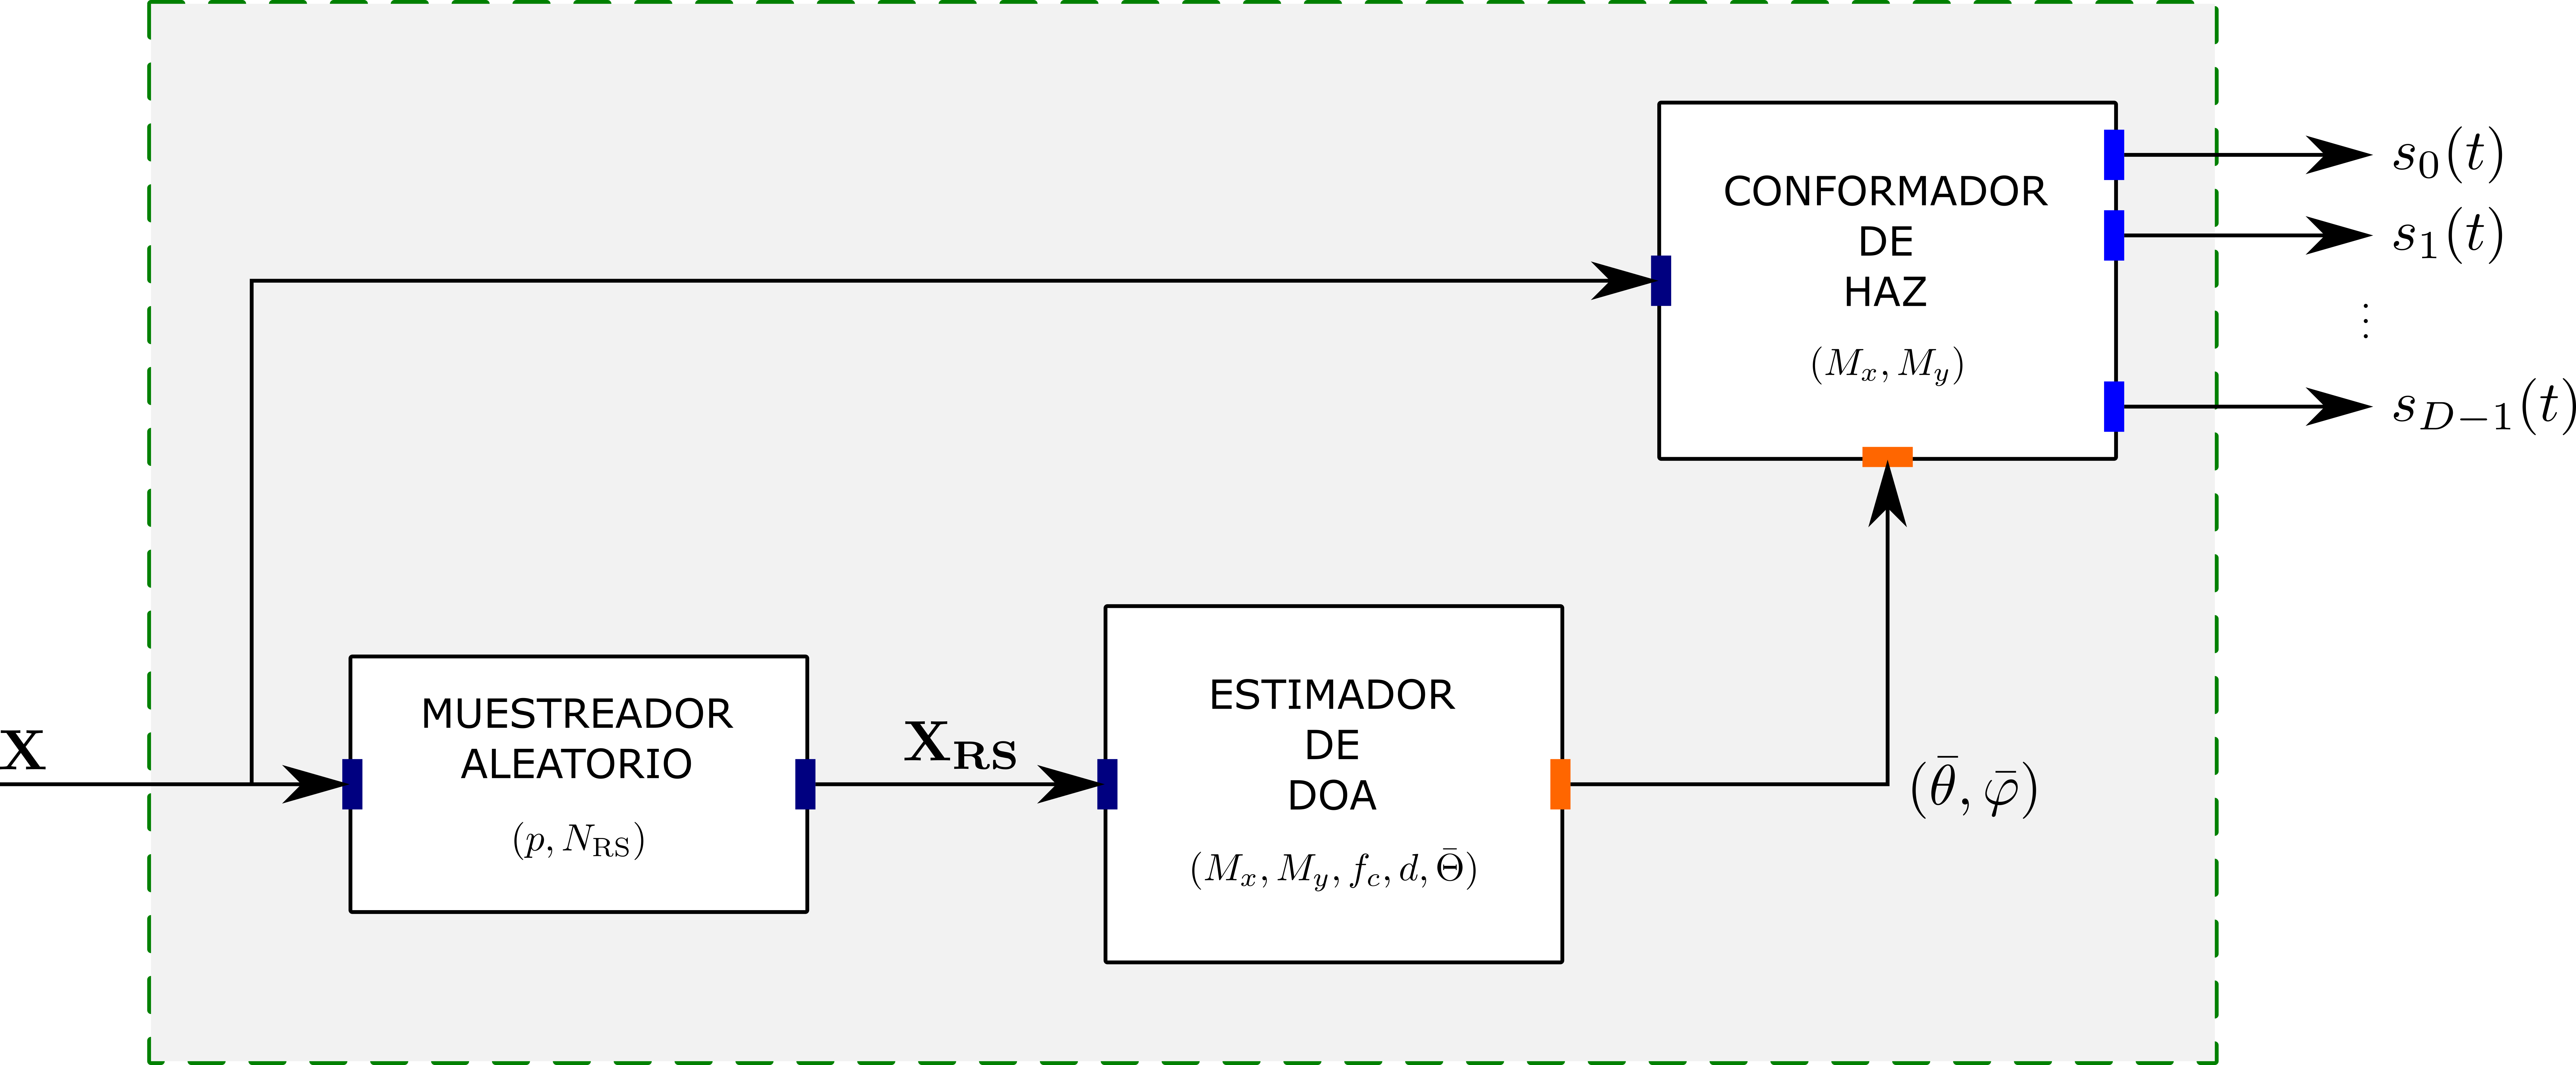
\includegraphics[width=0.9\linewidth]{images/06-Sistema/sistema_bd.png}
    \caption{Diagrama de bloques del sistema conformador de haz.}
    \label{fig:sistema_bd}
\end{figure}

Antes de operar el sistema debe ser configurado con los siguientes parámetros:
\begin{itemize}
    \item $M_x$: cantidad de elementos del arreglo de antenas en la dirección $x$.
    \item $M_y$: cantidad de elementos del arreglo de antenas en la dirección $y$.
    \item $f_c$: frecuencia nominal de portadora de las señales que se esperan recibir.
    \item $d$: distancia de separación entre elementos.
    \item $p$: probabilidad de tomar un vector de muestras en el muestreo aleatorio.
    \item $\bar{\Theta}:$ vector de parámetros del clasificador SVM obtenido mediante entrenamiento del algoritmo.
\end{itemize}

Este sistema puede ser implementado completamente en el PS, sin embargo la implementación de algunos de estos tres bloques en la FPGA puede llegar a traer alguna ganancia de rendimiento mediante la paralelización de cálculos, principalmente a medida que se aumenta la cantidad de señales recibidas, sin embargo al realizar esto se debe tener cuidado con las interfaces que se agregan entre el PS y la PL, ya que pueden llegar a ser un cuello de botella en el proceso, como así también hay que tener en cuenta la cantidad de recursos que quedan libres en la FPGA luego de que se instale el sistema de adquisición.

\section{Muestreador aleatorio}\label{subc:sistema_randomsampler}

El subsistema muestreador aleatorio recibe la matriz de muestras complejas $\mathbf{X}$ de tamaño $M \times N$ desde el sistema de adquisición y entrega una matriz de muestras $\mathbf{X_{RS}}$ de tamaño $M \times N_{\textrm{RS}}$ donde $N_{\textrm{RS}} = p\cdot N$. En este caso $p$ puede considerarse un factor de decimación, ya que es el número que define cómo se reduce la cantidad de muestras a la salida a partir de una cierta cantidad de muestras en la entrada. La matriz de salida se forma mediante elecciones aleatorias de las columnas de $\mathbf{X}$, utilizando el método que se explica en el Capítulo \ref{ch:randomsampling}.

\begin{figure}[ht!]
    \centering
    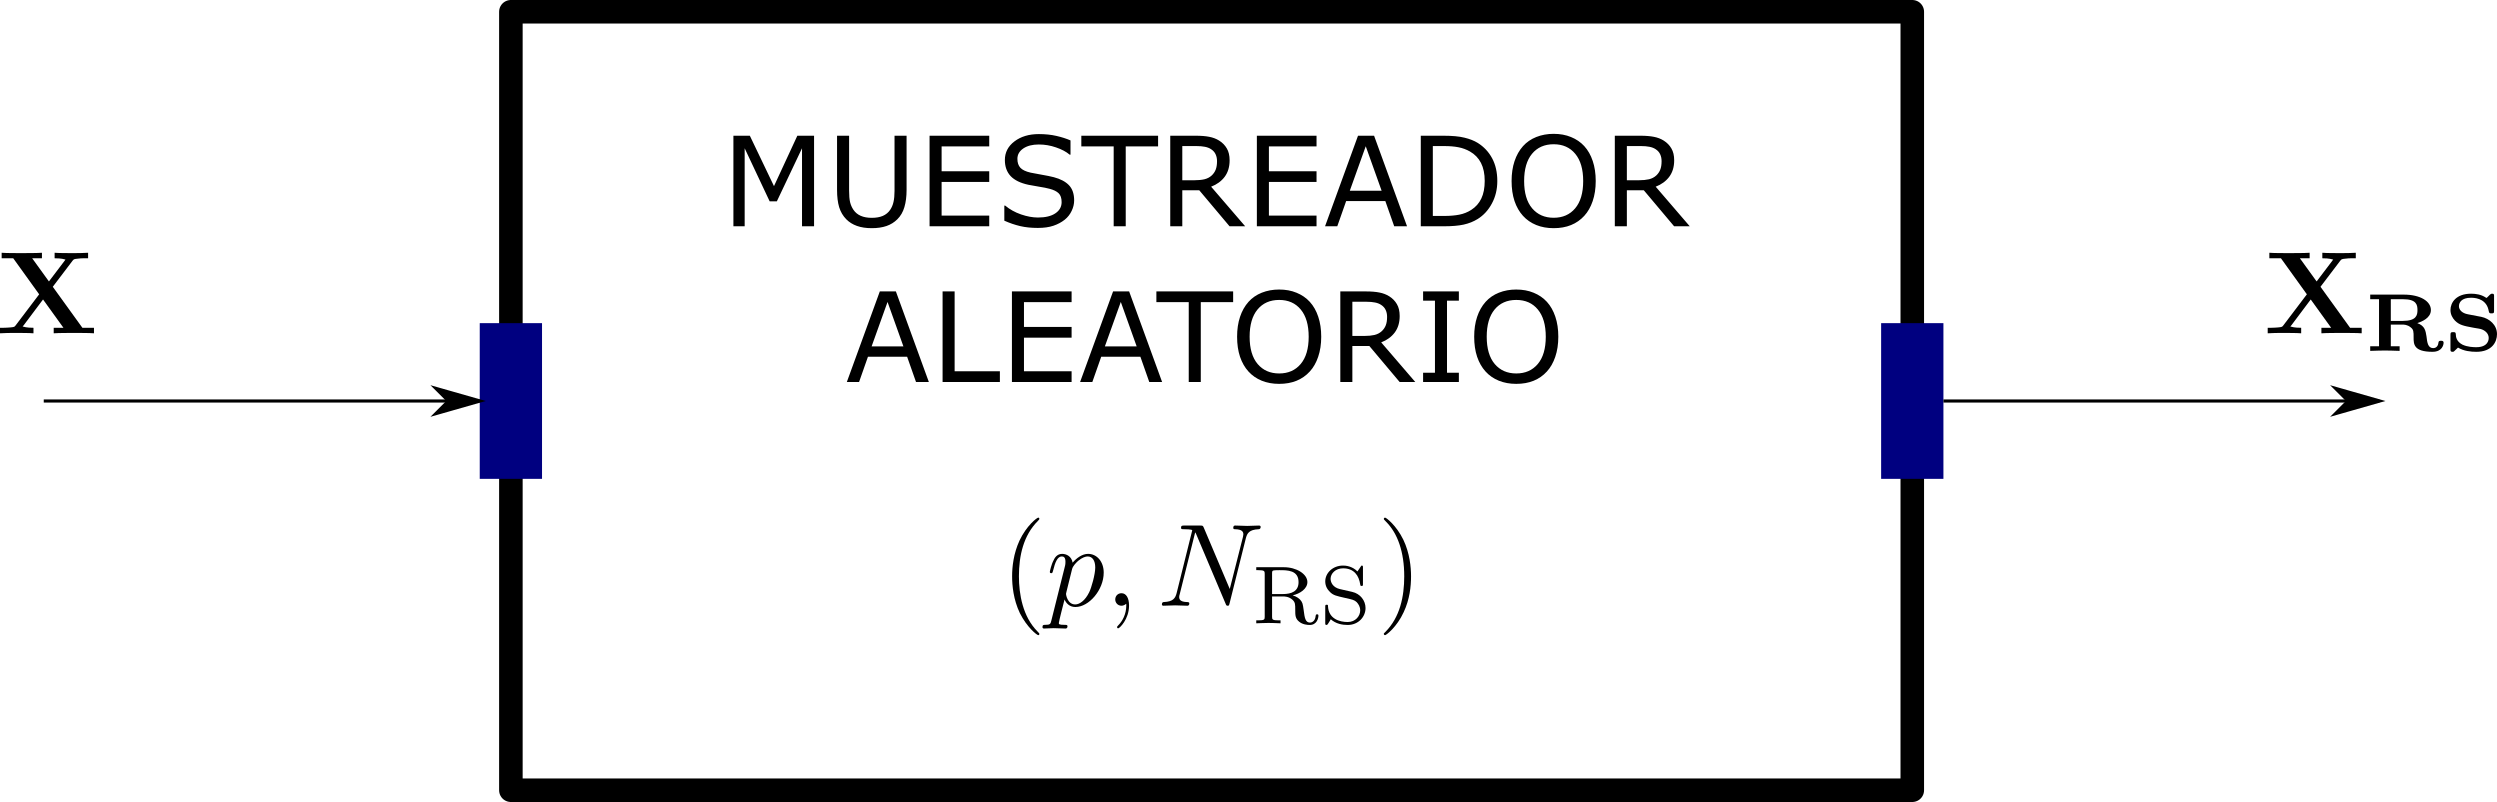
\includegraphics[width=0.6\linewidth]{images/06-Sistema/sistema_randomsampler.png}
    \caption{Representación en bloque del muestreador aleatorio con sus interfaces.}
    \label{fig:sistema_randomsampler}
\end{figure}

Otra manera de implementarlo es haciendo que este bloque reciba solo vectores de tamaño $M \times 1$ y que estos vectores se muestren en la salida con probabilidad $p$. Esta implementación evita tener que operar con matrices de tamaño $M \times N$.

\subsection{Implementación en FPGA}

Debido a que este módulo trabaja directamente con las muestras que entrega el sistema de adquisición, el contar con las muestras de cada elemento almacenadas en registros en la PL \cite{bib:jiqdc} permite una implementación rápida de este bloque que puede significar un ahorro de recursos en el PS, ya que, ubicando el muestreador aleatorio fuera del PS, se podría pensar en una implementación en el que este esté trabajando siempre con matrices de tamaño $M\times N_{\textrm{RS}}$ y no $M\times N$, reduciendo el consumo de memoria y los tiempos de carga de datos. A partir de esto, en la Figura \ref{fig:sistema_randomsampler_fpga} se muestra el diseño de bloques de una propuesta de implementación de este módulo en FPGA.

\begin{figure}[ht!]
    \centering
    \includegraphics[width=0.9\linewidth]{images/06-Sistema/sistema_randomsampler_fpga.png}
    \caption{Diseño de bloques de la propuesta de implementación del muestreador aleatorio en la FPGA.}
    \label{fig:sistema_randomsampler_fpga}
\end{figure}

Este diseño cuenta con 16 FIFOs \footnote{\emph{First in, first out}: bloque que permite el almacenamiento y la lectura de datos de manera tal que el primer dato en ser almacenado sea el primero en ser leído.}, una por cada elemento del ARU, capaces de almacenar una cantidad $N_{\textrm{RS}}$ de datos de 32 bits, suponiendo (sin pérdida de generalidad) que estos datos almacenan la parte real y la parte imaginaria de una muestra en porciones de 16 bits para cada una. Cada FIFO tiene una señal \texttt{FULL} que sirve para indicar al subsistema estimador de DOA el momento en el que las muestras se encuentran listas para ser procesadas, instante en el cual este subsistema puede levantar la señal de lectura para comenzar con la carga de los datos. La escritura de las FIFOs se realiza simultáneamente a partir de una señal externa que indica cuándo existen datos válidos en las entradas, y una señal interna generada a partir de la comparación de dos números de 16 bits: el número $p$ fijado por el usuario y otro número generado aleatoriamente cada tiempo de reloj por un bloque generador de números aleatorios. De esta manera, las FIFOs se cargan en tiempos aleatorios pero de manera simultánea entre ellas, entregando en sus salidas en el momento de lectura los vectores de la matriz $\mathbf{X_{RS}}$ que se muestra en la Figura \ref{fig:sistema_randomsampler}. En este caso no se utiliza la señal de \texttt{EMPTY} de las FIFOs ni se evita la escritura en las mismas cuando la señal \texttt{FULL} se encuentra en alto debido a que se busca que las FIFOs se encuentren actualizadas en todo momento con las muestras más recientes, ya que en esas muestras se encontrará la información de la DOA, la cual se desea mantener siempre actualizada. El único momento en el cual se debe impedir la escritura de datos es el momento en el que el subsistema estimador de DOA se encuentra haciendo la lectura de los datos que se encuentran dentro de las FIFOs.

\section{Estimador de dirección de arribo}\label{subc:sistema_doa_estimator}

El subsistema estimador de dirección de arribo, cuya representación como bloque se muestra en la Figura \ref{fig:sistema_doaest}, es el subsistema más complejo de los tres debido a las operaciones que realiza. Como se muestra en la Figura \ref{fig:sistema_doaest_2}, está conformado por 3 bloques:

\begin{itemize}
    \item \textbf{SVD:} bloque encargado de realizar la descomposición en valores singulares de la matriz de entrada $\mathbf{X_{RS}}$, obteniendo la matriz de valores singulares $\mathbf{\Sigma}$ y los vectores singulares izquierdos $\mathbf{E}$.
    \item \textbf{SVM:} bloque encargado de realizar la estimación de la cantidad de señales recibidas $D$ realizando una clasificación de los valores singulares contenidos en la matriz $\mathbf{\Sigma}$ utilizando el algoritmo de Máquina de Vectores de Soporte que se analizó en la Sección \ref{subc:ml_svm}. Utilizando un kernel gaussiano, el vector $\bar{\Theta}$ debe incluir, además, los parámetros adicionales $C$ y $\gamma$.
    \item \textbf{ESPRIT:} bloque encargado de realizar la estimación de DOA de las $D$ señales recibidas a partir de los vectores singulares izquierdos de la matriz $\mathbf{E}$. En su salida entrega los vectores $\bar{\theta}$ y $\bar{\varphi}$ de tamaño $D\times 1$.
\end{itemize}

Debido a la dinámica en el tamaño de los datos con los que opera este subsistema, ya que un cambio en la cantidad de señales recibidas implica un cambio en la cantidad de columnas con las que debe operar el bloque ESPRIT, y a la dificultad de implementar los algoritmos algebraicos de los bloques SVD y SVM en FPGA, comparada con la escasa dificultad de implementarlos en software, este sistema debe ubicarse en el PS.
\begin{figure}[ht!]
    \centering
    \begin{subfigure}[b]{0.5\textwidth}
        \centering
        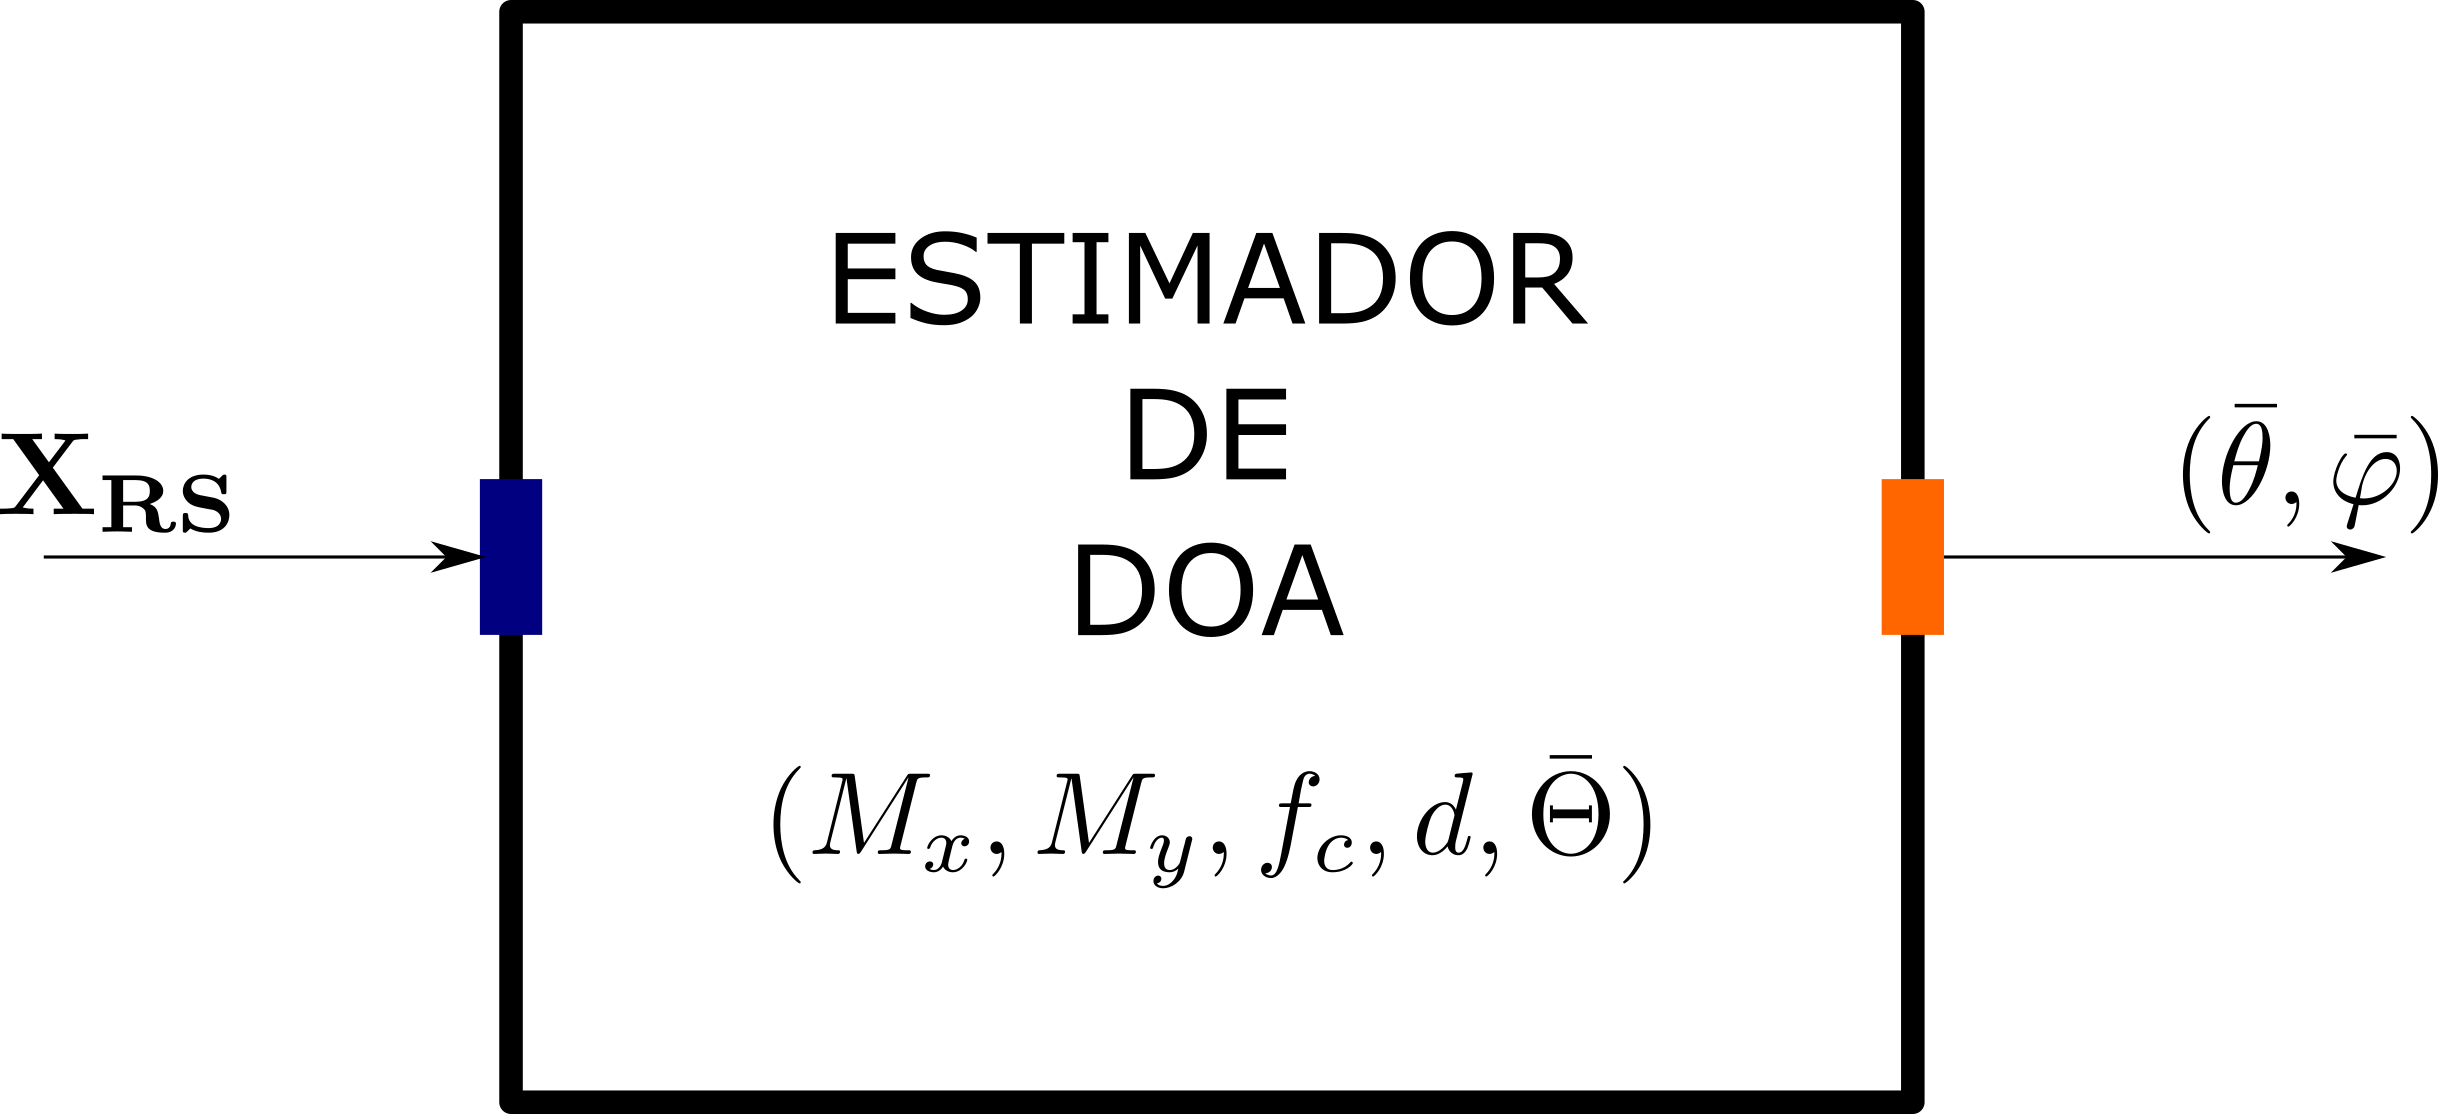
\includegraphics[width=\linewidth]{images/06-Sistema/sistema_doaest.png}
        \caption{Bloque.}
        \label{fig:sistema_doaest}
    \end{subfigure}
    \hfill
    \begin{subfigure}[b]{0.9\textwidth}
        \centering
        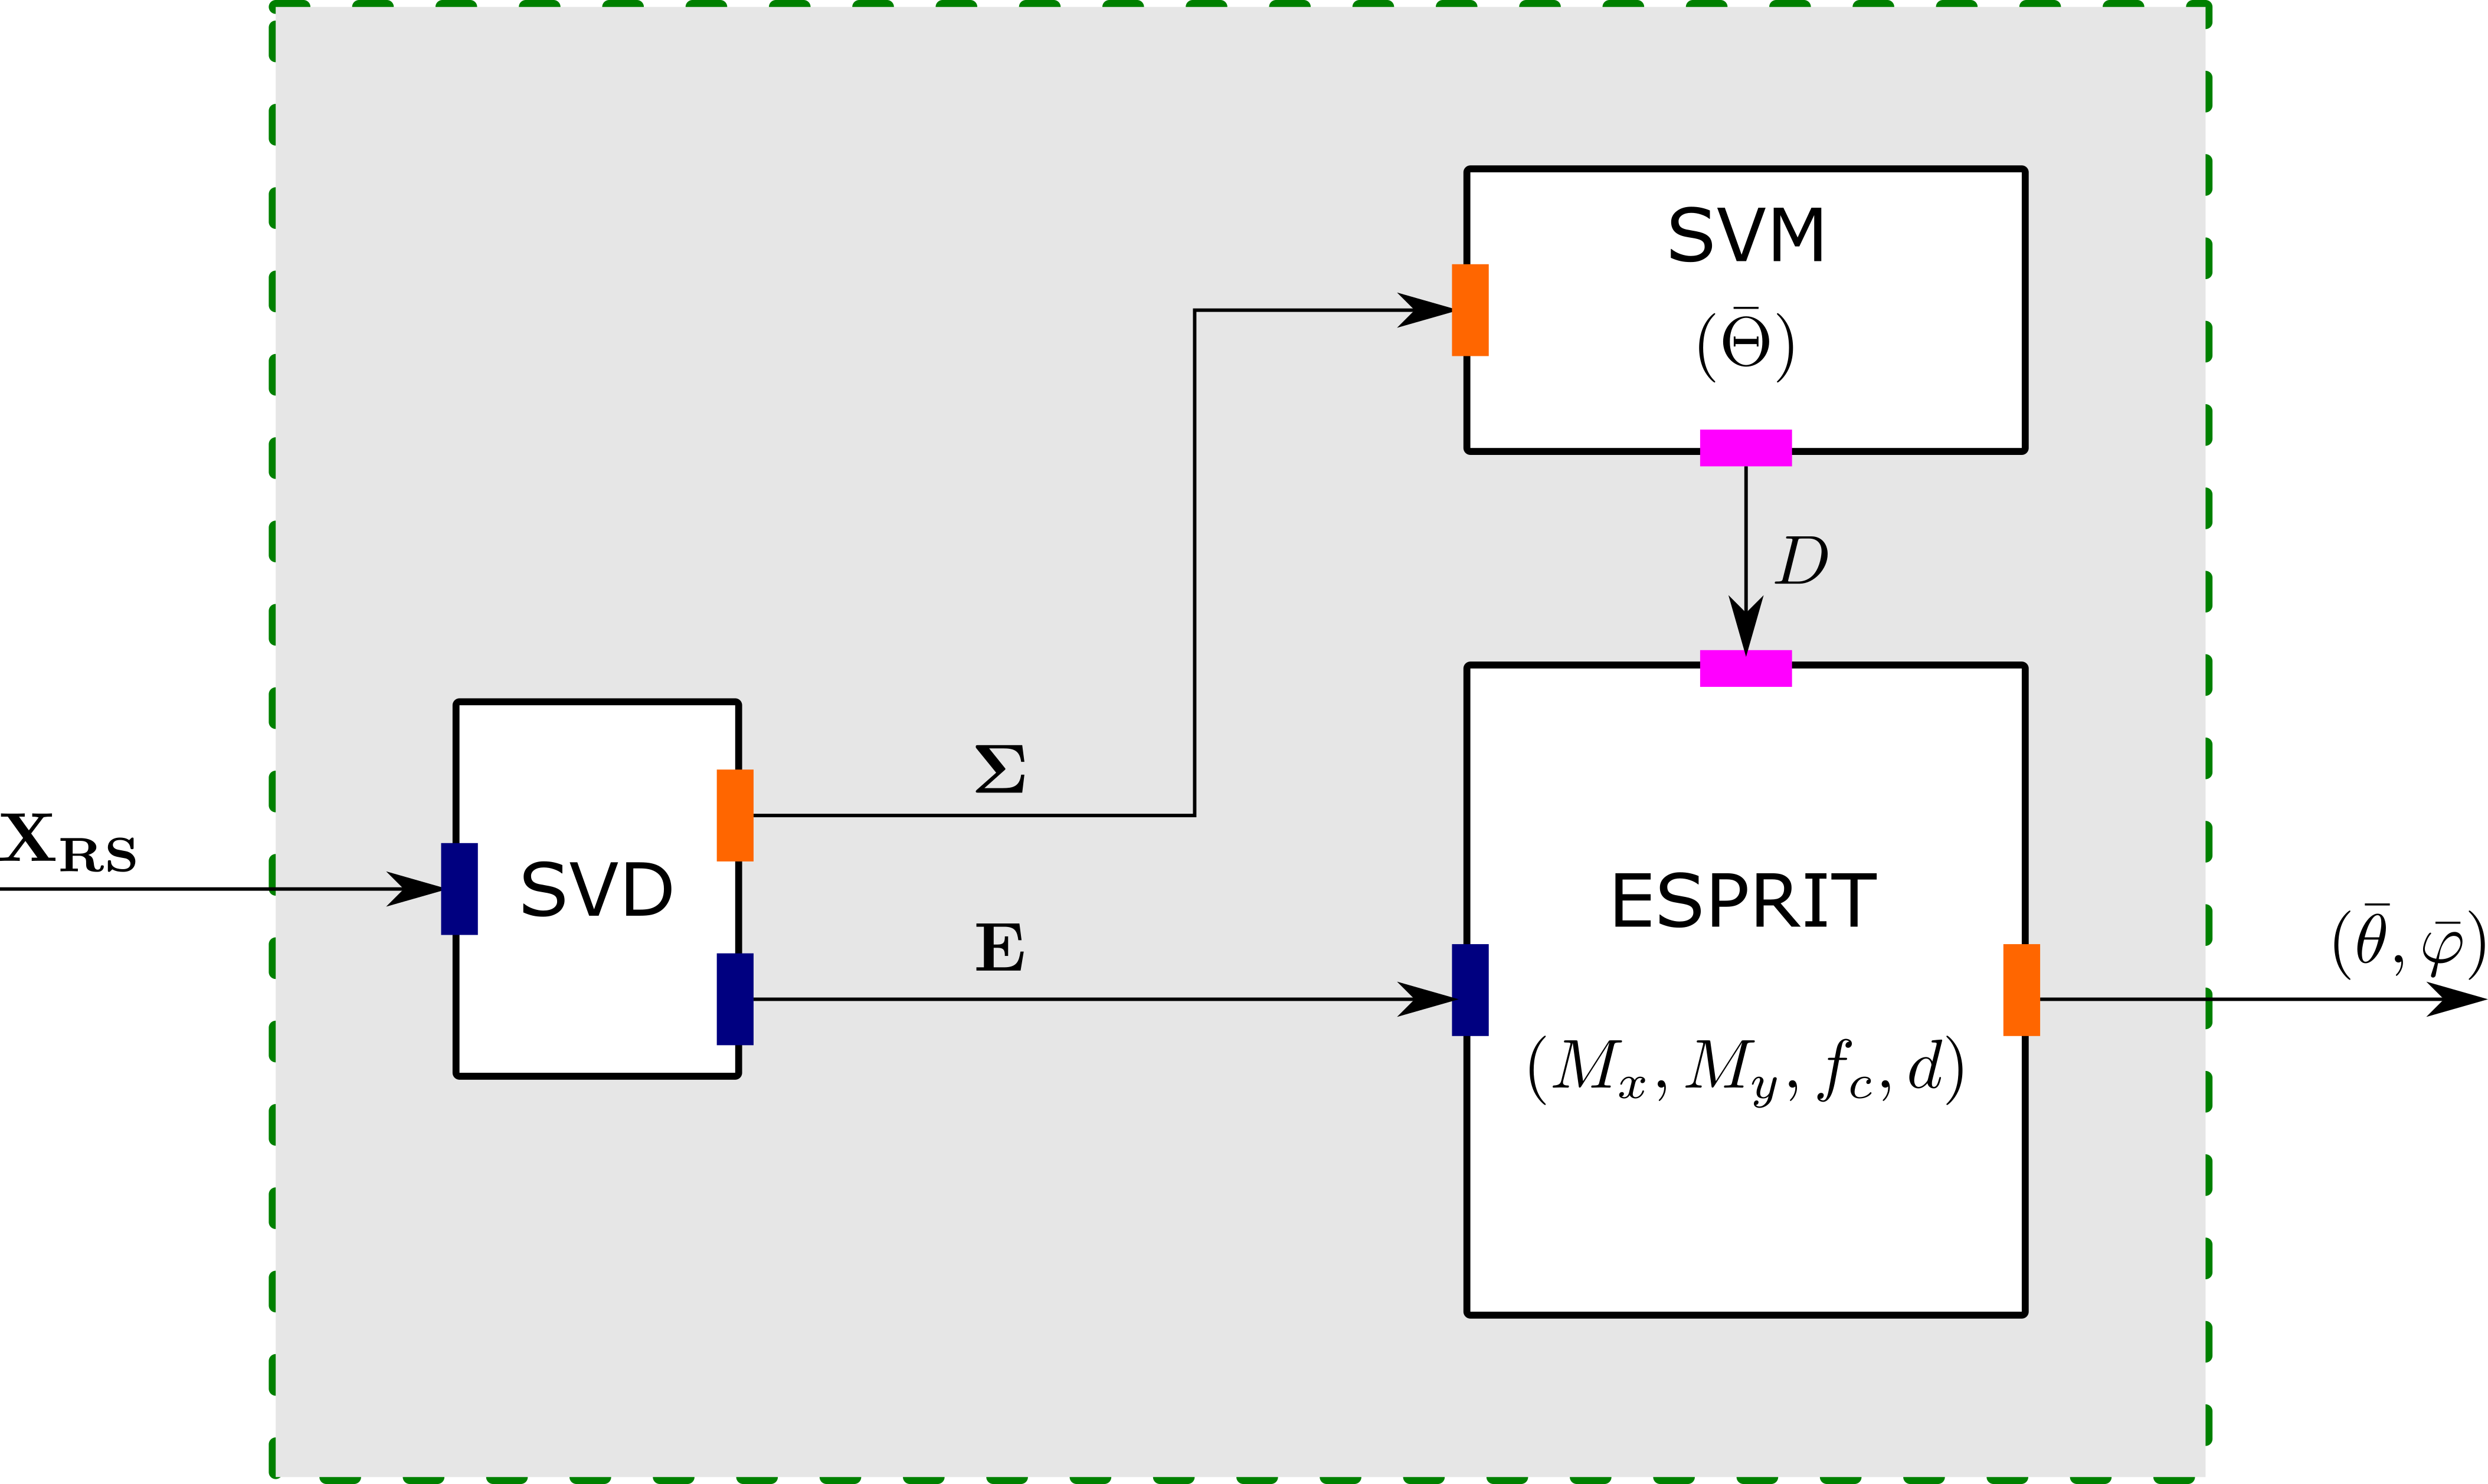
\includegraphics[width=\linewidth]{images/06-Sistema/sistema_doaest_2.png}
        \caption{Detalle del subsistema.}
        \label{fig:sistema_doaest_2}
    \end{subfigure}
    \caption{Representación como bloque del subsistema estimador de DOA con sus correspondientes interfaces.}
\end{figure}



\section{Conformador de haz}\label{subc:sistema_beamformer}

El último subsistema a implementar es el conformador de haz, cuya representación en bloque se muestra en la Figura \ref{fig:sistema_beamformer}. Con la información obtenida de los otros dos subsistemas, el conformador de haz se encarga de procesar las muestras de cada elemento del ARU restándole la diferencia de fase con respecto al elemento de referencia y promediando todas las muestras de manera tal de obtener las $D$ señales a la salidas. Además, si se conoce el patrón de radiación de cada elemento del ARU puede afectarse a cada muestra por la ganancia del arreglo en la DOA para normalizar las señales recibidas. Por cada señal detectada la operación que realiza este subsistema es la siguiente:

\begin{align}
    \hat{s_d}[n] & =\frac{1}{M\left(g(\hat{\theta}_d,\hat{\varphi}_d)\right)^2}\cdot\bar{a}_{\textrm{ARU}}^H(\hat{\theta}_d,\hat{\varphi}_d) \cdot \bar{x} \\
                 & =\frac{1}{M\cdot g(\hat{\theta}_d,\hat{\varphi}_d)} \cdot \begin{bmatrix}
        1 & \cdots & e^{jkd[(M_x-1)\cos \hat{\theta}_d \cos \hat{\varphi}_d+(M_y-1)\cos \hat{\theta_d} \sin \hat{\varphi}_d]}
    \end{bmatrix} \cdot \begin{bmatrix}
        x_0 \\
        x_1 \\
        x_{M-1}
    \end{bmatrix}    \nonumber      \\
                 & = \frac{1}{M\cdot g(\hat{\theta}_d,\hat{\varphi}_d)} \sum_{m=0}^{M-1} a_m^*(\hat{\theta}_d,\hat{\varphi}_d) \cdot x_m,\nonumber
\end{align}
con $d=0,1,...,D-1$ y donde $\bar{a}_{\textrm{ARU}}$ es el vector de apuntamiento definido en la Ecuación \ref{eq:beamforming_a_aru}

\begin{figure}[ht!]
    \centering
    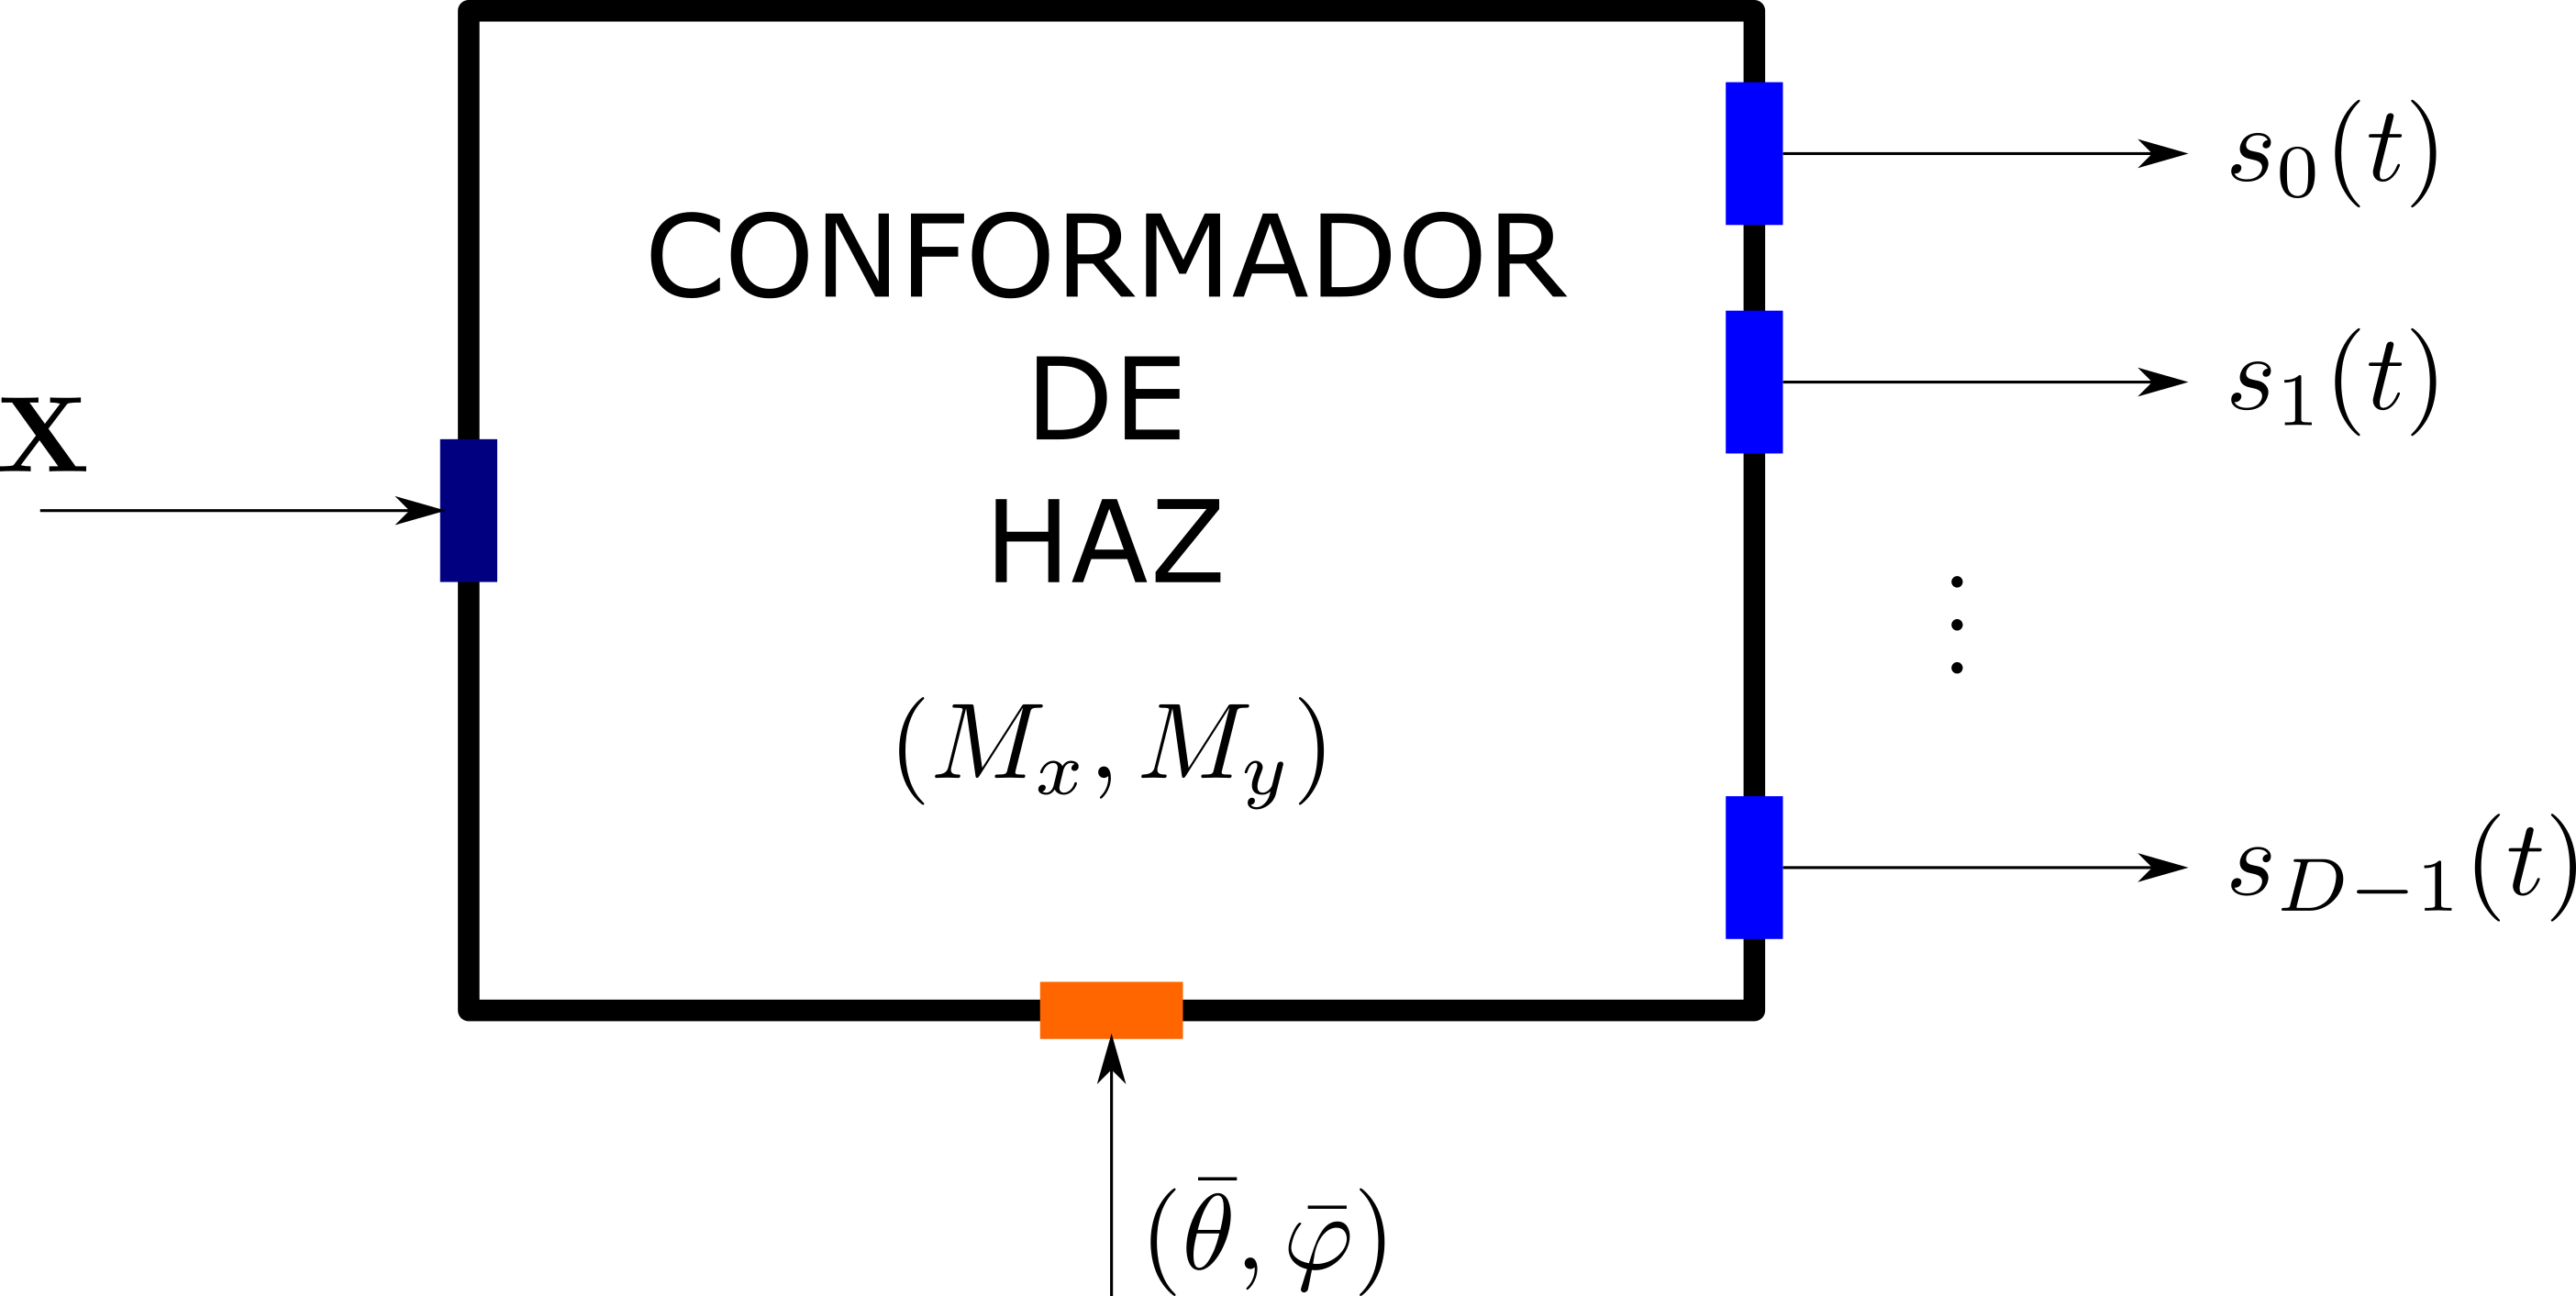
\includegraphics[width=0.5\linewidth]{images/06-Sistema/sistema_beamformer.png}
    \caption{Representación como bloque del subsistema conformador de haz con sus correspondientes interfaces.}
    \label{fig:sistema_beamformer}
\end{figure}

\subsection{Implementación en FPGA}

Este algoritmo puede ser implementado tanto en el PS como en la FPGA, debido a que no requiere realizar cálculos de mayor complejidad. Una ventaja de implementarlo en la PL junto al muestreador aleatorio es, como ya se mencionó, evitar que el PS tenga que manipular matrices de tamaño $M\times N$ y en su lugar trabajar con matrices $M\times N_{\textrm{RS}}$ donde $N_{\textrm{RS}}$ puede ser incluso más de dos órdenes de magnitud menor que $N$. En la Figura \ref{fig:sistema_beamformer_fpga} se muestra un diagrama de bloques de una propuesta de implementación de este subsistema en FPGA.

\begin{figure}[ht!]
    \centering
    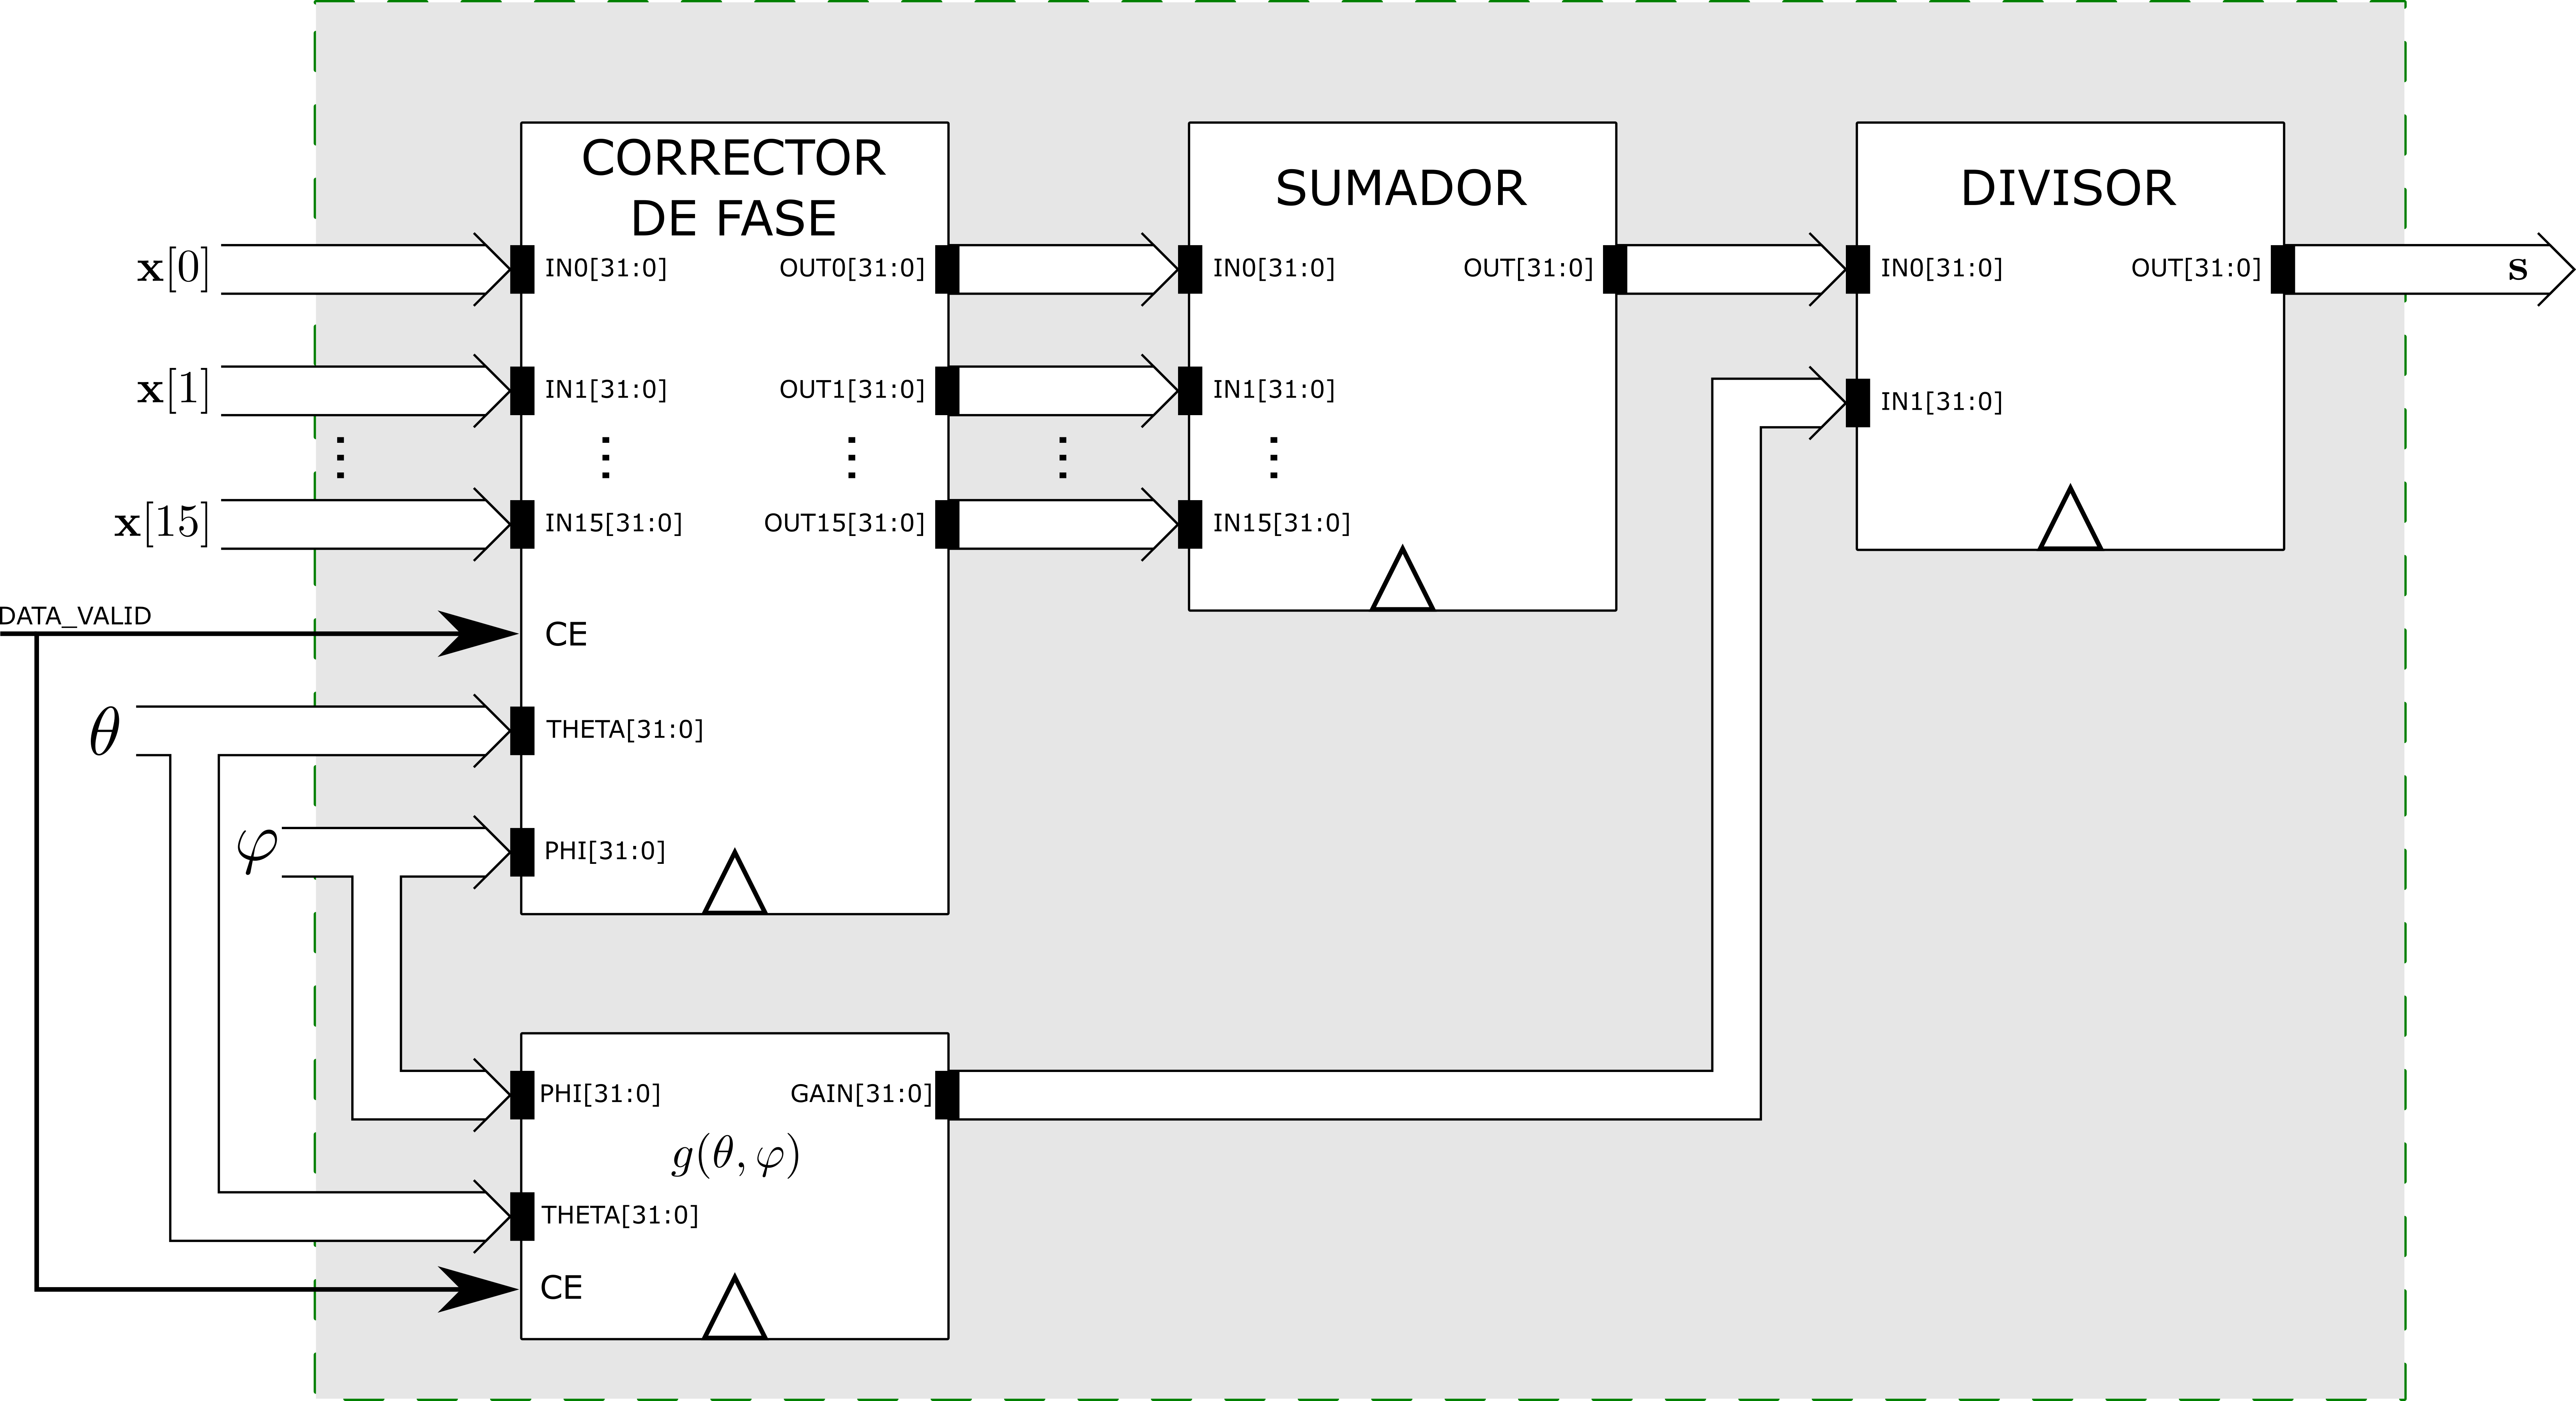
\includegraphics[width=0.9\linewidth]{images/06-Sistema/sistema_beamformer_fpga.png}
    \caption{Propuesta de implementación del subsistema conformador de haz en FPGA.}
    \label{fig:sistema_beamformer_fpga}
\end{figure}

En este diseño el sistema recibe como entradas las 16 muestras de 32 bits provenientes del sistema de adquisición, los ángulos de elevación y azimut provenientes del subsistema estimador de DOA (el cual se encuentra en el PS), y una señal de validación proveniente del PS que indica el instante en el que existen ángulos de arribo válidos en las correspondientes entradas. Dentro del subsistema existen cuatro bloques: un corrector de fase, el cual se encarga de restar la fase de cada muestra dependiendo de con qué elemento fue tomada, un bloque sumador que suma las 16 salidas del bloque corrector de fase para realizar el promediado de la señal recibida, un bloque que a partir de una DOA entrega la ganancia del ARU en esa dirección, y un divisor que utiliza esta ganancia para normalizar la señal recibida. Siendo que en este caso la cantidad de elementos del ARU es 16, el promediado puede hacerse quitando los 4 bits menos significativos de esta salida. Hay que notar que este diseño solo sirve para realizar la conformación de haz de una única señal, en caso de aumentar las salidas del sistema debe repetirse este bloque y alimentarlo con las direcciones de arribo de las señales restantes. Esta es una desventaja de la implementación en la PL, ya que el diseño no puede ser dinámico según la información recibida y debe ser dimensionado para el peor caso.
\chapter{GNURadio}\label{ch:gnuradio}
%\chapterquote{Hablaban siempre de dinero y planeaban asaltar un banco}{Domingo Cavallo, 2001}

\section{Conceptos generales}\label{subc:intro_congen}



%\chapter{Propuesta de diseño en FPGA}\label{ch:fpga}
%\chapterquote{Hablaban siempre de dinero y planeaban asaltar un banco}{Domingo Cavallo, 2001}
%hablar de las posibilidades de mejorar el cálculo en cosas paralelizables

\section{Conceptos generales}\label{subc:fpga_congen}



\chapter{Trabajo a futuro}\label{ch:futuro}
\chapterquote{To my future descendants: I have lent to Miss Bloop's private museum, the Medallion and the Ancestral Tunic which rightfully belong to you.}{Twinsen}

En este capítulo se hace una breve mención del trabajo que resta por hacer para completar la implementación del sistema conformador de haz, así como también posibles alternativas de implementación que no fueron estudiadas a lo largo de este proyecto y que pueden mejorar el producto final.

\section{Interfaz e integración con el sistema de adquisición}\label{subc:futuro_interfaz}
Como se mencionó en el Capítulo \ref{ch:sistema}, el fin de este sistema es ser implementado en una placa de desarrollo CIAA-ACC, sobre la cual va a estar instalado, también, el sistema de adquisición de muestras del ARU. Estos dos sistemas deben estar comunicados, de manera tal que el sistema de adquisición pueda enviar las muestras al sistema conformador de haz. Debido a que el conformador de haz tendrá parte de su implementación en el PS y parte de su implementación en la PL, es necesario definir las interfaces y el protocolo que utilizarán para la comunicación. En el chip Xilinx Zynq-7030, el PS puede comunicarse con la PL a través de un bus AXI-Lite, en el cual el PS toma el rol de maestro y la PL de esclavo. Por esto, es intuitivo pensar que dentro de la FPGA el sistema adquisidor y los bloques muestreador aleatorio y conformador de haz pueden tomar el rol de esclavos AXI y ser comandados por software a través del PS para redirigir las muestras al bloque estimador de DOA. Por otro lado, se puede evaluar el uso de una interfaz directa entre el sistema adquisidor y los bloques conformador de haz y muestreador aleatorio, ya que estos bloques deberán poder tener acceso simultáneamente a los registros del sistema adquisidor donde se almacenan las muestras de los elementos. Asegurarse una conexión punto a punto entre estos bloques es un criterio de diseño primordial para asegurar el mayor rendimiento del sistema. Finalmente, la interfaz entre el maestro AXI y el bloque estimador de DOA, dentro del PS, puede utilizar una interfaz UDP, debido a su simplicidad de implementación y a que en esta interfaz no se requiere verificar la integridad de los datos transmitidos. Además, si se decide utilizar GNU Radio para la ejecución de este bloque, este cuenta con una interfaz UDP que puede ser instanciada fácilmente con un bloque. En este caso deberá definirse, además, un protocolo de empaquetamiento de los datos transmitidos. En la Figura \ref{fig:futuro_interfaz} se muestra un esquema de esta propuesta.

\begin{figure}[ht!]
    \centering
    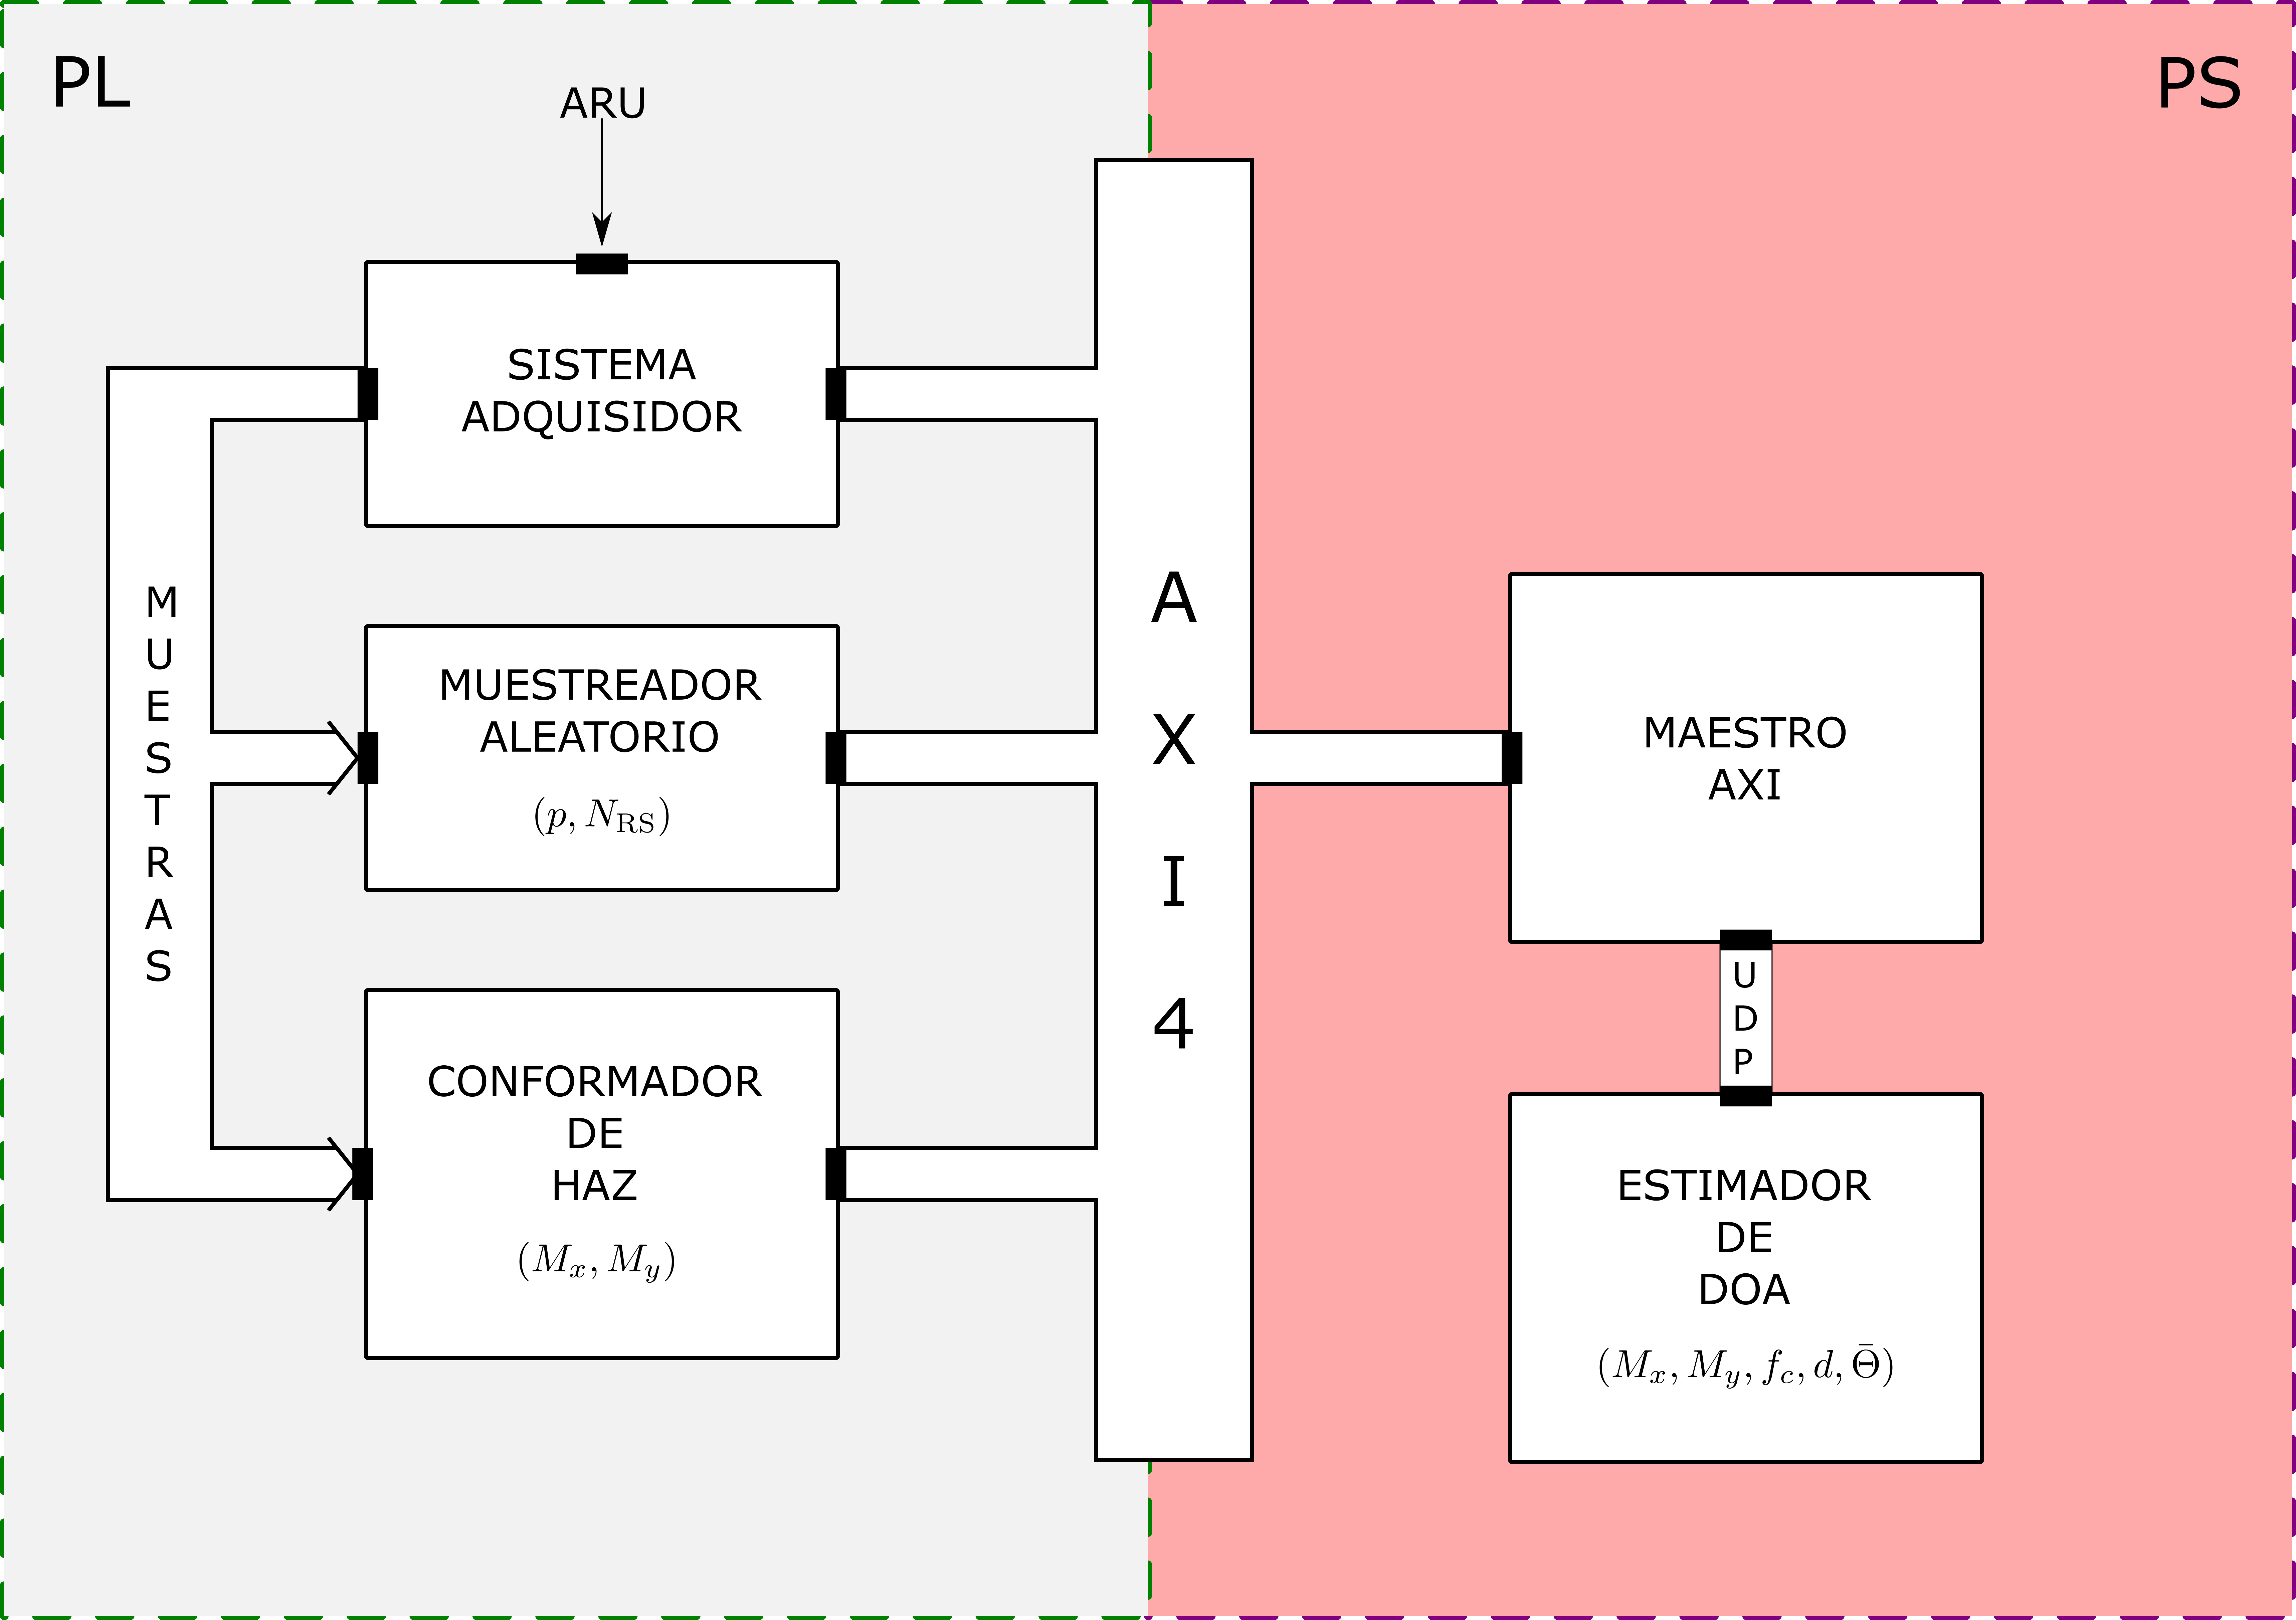
\includegraphics[width=0.9\linewidth]{images/08-Futuro/futuro_interfaz.png}
    \caption{Propuesta de interfaz para la integración del sistema conformador de haz con el sistema de adquisición.}
    \label{fig:futuro_interfaz}
\end{figure}

\section{Carga del patrón de radiación del arreglo}\label{subc:futuro_patron}
Una vez construido el arreglo de antenas con el cual se equipará el sistema, y habiendo realizado una medición de su patrón de radiación, debe cargarse esta información dentro del bloque conformador de haz para poder realizar la normalización de las muestras recibidas, como se mostró en la Sección \ref{subc:sistema_beamformer}.

\section{Interferencias destructivas}
Como se nombró en el Capítulo \ref{ch:beamforming}, la técnica de conformación de haz no solo permite realizar la recepción o transmisión direccional de señales sino que también permite generar mínimos en el patrón de radiación de manera tal de poder suprimir interferencias direccionales. La manera de generar estos mínimos es aplicando distintos pesos a las muestras provenientes de los elementos del arreglo. Una vez conocida la dirección de la interferencia, los pesos a aplicar pueden obtenerse mediante la resolución de un sistema de ecuaciones.

\section{Smart Beamforming}\label{subc_smartbeamforming}
Si bien el algoritmo que se desarrolló en este proyecto puede considerarse de alguna manera ``inteligente'' debido a que es capaz de deducir por su cuenta la dirección de arribo de señales, el término \emph{Smart Beamforming} hace referencia a técnicas de conformación de haz que utilizan algoritmos de inteligencia artificial para la estimación de DOA y la conformación de las señales arribantes.
Actualmente ya existen estudios que demuestran la factibilidad técnica y la mejora en rendimiento al emplear algoritmos de estimación de DOA basados en inteligencia artificial y, particularmente, en redes neuronales \cite{bib:smart_beamforming}, lo cual motiva a tener en cuenta este tipo de análisis para futuras implementaciones.
\chapter{Conclusiones}\label{ch:conclusiones}
\chapterquote{He llegado hasta el fin, con los brazos cansados...}{Gustavo Cerati}

En este proyecto se realizó el estudio de distintas técnicas de implementación de un conformador de haz digital adaptativo, partiendo de una introducción teórica sobre los conceptos en los que se basa esta técnica, identificando los distintos tipos de conformadores de haz, definiendo el concepto de arreglo de antenas en fase y caracterizando sus distintos tipos, para luego definir el problema a resolver. A partir de aquí se realizó el estudio de las distintas técnicas de estimación de DOA, componente primordial para el funcionamiento del sistema a implementar. En este estudio se definió el modelo de muestras que se utilizó a lo largo de todo el proyecto y se realizó una introducción teórica sobre los conceptos algebraicos que permiten la descomposición del subespacio de muestras en subespacios de señal y ruido. La comprensión de esta técnica permitió iniciar con el análisis de dos algoritmos populares en lo que respecta a la estimación de parámetros de señales recibidas en arreglos de sensores: MUSIC y ESPRIT. Durante este estudio se desarrolló la teoría en la que se basa el funcionamiento de ambos algoritmos para finalmente realizar implementaciones de ambos que permitieron su comparación. En este estudio, MUSIC demostró ser un excelente algoritmo para introducirse en el análisis de técnicas de estimación paramétrica de señales debido a su intuitivo enfoque gráfico. Sin embargo, al momento de la implementación, ESPRIT demostró ser superior en lo que respecta a tiempos de ejecución, alcanzando niveles de error prácticamente idénticos. A partir de esto se decidió continuar con el algoritmo ESPRIT para el resto de la implementación.

Durante la realización de las simulaciones de los algoritmos de estimación de DOA implementados se observó que en situaciones particulares en las que las señales recibidas se encontraban muy correlacionadas se requería operar con una cantidad de muestras que volvía inviable la implementación de un sistema en tiempo real. A partir de aquí se logró dar con una técnica de muestreo aleatorio que dio excelentes resultados al momento de reducir la cantidad de muestras requeridas para realizar la estimación de DOA, reduciendo dicho número por encima de dos órdenes de magnitud. Luego de comprobar su correcto funcionamiento se logró dar con una explicación teórica de su eficacia, la cual se indica en el Capítulo $\ref{ch:randomsampling}$.

Para resolver el problema de estimación de cantidad de señales recibidas se observó que se podían utilizar técnicas de clasificación mediante aprendizaje automático. A partir de esto se pudo implementar un algoritmo que permitió realizar la clasificación de valores singulares, necesaria para realizar la estimación de cantidad de señales recibidas, el cual al ser comparado con el método de la máxima derivada, que consiste en hallar el umbral de separación entre valores singulares encontrando la máxima derivada de esta distribución discreta, mostró una mejora del 10\%, alcanzando una precisión de 97\%.

Una vez definidos los subsistemas que componen el conformador de haz se realizó un diseño de bloques, definiendo la función y las interfaces de cada uno de ellos, realizando un análisis cualitativo de las ventajas y desventajas que existen al implementar ciertas funciones en FPGA o en el PS. Finalmente se esboza una propuesta de diseño de bloques para FPGA para una futura implementación.

Por último se realizó una implementación en GNU Radio del sistema conformador de haz completo, validando su funcionamiento mediante simulaciones. Diseñando las interfaces necesarias, este software puede ser instalado en el PS de la placa de desarrollo para realizar pruebas iniciales cuando se construyan el resto de los sistemas que complementan al conformador de haz (sistema de adquisición y arreglo de antenas).

Como cierre de este trabajo se esbozaron algunas propuestas de estudio e implementación a futuro con el objetivo de motivar la continuación de este proyecto analizando alternativas que pueden llegar a conseguir resultados aún mejores a los obtenidos.


\appendix
\chapter{Apéndice I}\label{C:ap1}
%\chapterquote{Negociemos Don Inodoro}{Fernando de la R\'{u}a, 2001}
\graphicspath{{figs/}}
%%%%%%%%%%%%%%%%%%%%%%%%%%%%%%%%%%%%%%%%%%%%%%%%%%%%%%%%%%%%%%%%%%%%%%%%



%%% Local Variables: 
%%% mode: latex
%%% TeX-master: "template"
%%% End: 


\begin{biblio}
    \bibliography{mibib}
\end{biblio}


\begin{postliminary}

    %\begin{seccion}{Publicaciones asociadas}
    %    \begin{enumerate}
    %        \item Mi primer aviso en la revista \textbf{ABC}, 1996
    %        \item Mi segunda publicaci\'{o}n en la revista \textbf{ABC}, 1997
    %    \end{enumerate}
    %\end{seccion}

    \begin{seccion}{Agradecimientos}
        Este documento lleva incluido una sumatoria de esfuerzos y ayudas de personas que no figuran como autores, pero que sin su aporte muy probablemente hoy no estuviese sentado aquí, escribiendo las últimas palabras que dan cierre a mi carrera universitaria.

        En primer lugar debo agradecer a Santiago y Nicolás, los directores de este proyecto, quienes jamás pusieron traba alguna a la hora de brindarme una ayuda o un consejo sobre cómo encarar el desarrollo del mismo. Sin ustedes esta tesis no sería ni la mitad de lo que es. Espero haber estado a la altura.

        A los jurados, Roberto y Damián, quienes tuvieron la difícil tarea de hacerse un tiempo para leer y corregir las casi 90 páginas de este documento. Ojalá que entre tantas ecuaciones y figuras hayan encontrado algún momento de diversión durante la lectura.

        A Diego, quien fue mi tutor desde el inicio de mi carrera en el instituto, y con quien jamás tuve alguna conversación que no fuera, cuanto menos, interesante. Gracias por haberme dado las palabras de aliento en esos momentos en los que era difícil ponerse a estudiar y por nunca haber dejado de creer en mí.

        A las autoridades del Instituto Balseiro, los miembros de la Comisión de Ingreso que con solo levantarme el pulgar y darme un voto de confianza me dieron la oportunidad que cambió mi vida para siempre. A ambos directores de la carrera de Ingeniería en Telecomunicaciones que cumplieron funciones durante mi paso por el IB, Diego y Juan Pablo, quienes siempre trabajaron para llevar más cerca de la perfección una carrera que ya es excelente de por sí. Al personal del Centro Atómico, quienes colaboraron para que en poco tiempo haya logrado sentirlo como mi casa.

        A Federico La Rocca, quien apareció con su taller de GNU Radio en el momento justo para que pudiese implementarlo en el proyecto y terminar de darle la vuelta de tuerca que faltaba para cerrarlo.

        A Willy Güichal, quien aguantó un semestre entero dándome clases como alumno único en su materia, tanto en modalidad presencial como virtual, y quien, encima, tuvo el grandioso gesto de darme mi primer trabajo como ingeniero. Nunca voy a poder terminar de agradecerte lo suficiente.

        A Norbert, quien fue mi primer contacto con el instituto al ``apadrinarme'' y nunca le faltó algún consejo para hacerme un poco más llevadero mi paso por la carrera.

        A Martín, Agustín y David, Nahuel Y Kevin, mis primeros amigos universitarios que se mantuvieron firmes desde 2009 y con quienes nunca perdimos contacto. Gracias por esas juntadas de estudios, por esos apuntes prestados y por esas risas que nunca faltaron.

        A Joako, el amigo que más paciencia me tuvo y más ayuda me brindó durante toda mi carrera. Todas las noches que te quedaste hasta tarde en mi casa explicándome sobre circuitos de amplificación no fueron en vano.

        A Leo y Kero, mis amistades del pueblo desde la primaria, quienes cada vez que volvía parecía como si nos hubiésemos visto el día anterior. Gracias por haber mantenido la amistad.

        A Silvina, la profe que me acompañó durante y después de la secundaria, forjando mi amor por la física y los números, luego ayudándome laboralmente y finalmente apoyándome en la decisión de entrar al IB.

        Al staff de la Fundación Libertad, principalmente a Gerardo y a Ana, quienes dándome empleo durante 5 años me permitieron seguir estudiando para alcanzar esta meta, además de permitirme formarme como profesional.

        A Lucila, quien fue testigo de la última etapa de todo este proceso y fue capaz de aguantar conmigo todos los estados de ánimo por los que pasé. Siempre te voy a estar agradecido por eso.

        A Emma y a Lulo, mis hermanos de distinta familia desde hace 17 años, quienes no solo me incentivaron cuando les conté una noche de febrero de 2017 sobre mi idea de hacer el ingreso al IB, sino que incluso después de irme mantuvieron un contacto constante conmigo que me hizo sentir como si nunca nos hubiésemos alejado físicamente, lo cual demuestra cuán genuina es nuestra amistad.

        A mi abuela, quien con llamados casi semanales realizaba el seguimiento de mis avances y me alentaba a alcanzar la meta. Me alegra mucho que seas testigo de esto después de tanto tiempo.

        A Edgardo, quien a pesar de haber pasado los momentos más difíciles nunca dejó de acompañarme y ayudarme en lo que podía cada vez que lo necesité.

        Durante el transcurso de la carrera en el IB, si no están dadas ciertas condiciones uno puede pasar por momentos de mucha angustia por cuestiones que van más allá del apoyo y la contención que puede brindar la institución. Si no se tiene a alguien con quien compartir un momento, un pensamiento, una idea, o buscar una charla, una opinión, esta etapa puede volverse muy complicada, y si a mí no me ocurrió eso es gracias a mis compañeros telecos. Ustedes fueron ese apoyo que hizo que, no solo no me cueste vivir en el Centro Atómico, sino que además vivir en el instituto sea un gusto, y que esta etapa que hoy cerramos quede en mi memoria como una de las etapas más lindas de mi vida. Haber compartido estos 3 años y medio con ustedes fue el regalo más lindo de toda esta experiencia y no me imagino habiéndola pasado tan bien con personas distintas a ustedes. Fueron mi familia durante estos 3 años y medio y la van a seguir siendo de aquí en adelante.

        Tengo que agradecerte Laucha por tener el récord de ser la persona que más tiempo convivió conmigo sin tener jamás un problema. Hiciste que mi vida en el Balseiro sea mucho más fácil y agradable de lo que pudiese haber sido. Gracias por todos esos ratos de música que, por suerte, no fueron pocos.

        Ahora se me viene a la mente esa mañana en el trabajo cuando me llegó el correo que dio por iniciado el resto de mi vida, la emoción de mi hermana y el abrazo de mi hermano. La misma emoción y el mismo abrazo que me dieron en el aeropuerto el día que me despedí de ellos por primera vez. Siempre hicieron lo necesario para apoyarme y ayudarme durante mi experiencia en el IB, tanto a la distancia como este último año que tuvimos la oportunidad de volver a convivir juntos otra vez. Este logro es suyo también.

        Por último quiero agradecer a la primer responsable de todo esto, aquella persona que durante la primaria se quedaba hasta altas horas de la noche después de haber trabajado todo el día para enseñarme trucos para aprender más rápido las tablas de multiplicación o que restarle un número a otro era lo mismo que contar cuántos números le faltaban al más chico para alcanzar al más grande, quien se ponía la alarma a las 6 de la mañana para despertarnos para ir a la escuela aunque se había quedado trabajando hasta las 3, aquella persona que quizás no nos dio todo lo que quiso darnos, pero que siempre se esforzó para que nunca nos falte lo que ella creía que era lo más importante: la educación. Espero que este logro sea la prueba que demuestre que todo lo que hiciste fue lo correcto. Gracias mamá.

    \end{seccion}

\end{postliminary}

\end{document}

